\section{Artificial density bumps}\label{density_bump}




\subsubsection{Choice of initial radial flow}
The initial cylindrical radial velocity is motivated by the following
considerations. For axisymmetric flow with angular velocity that only
depends on the cylindrical radius, the azimuthal momentum equation reads
\begin{align}\label{ang_mom_cons}
  R\rho v_R\frac{\p}{\p R}\left(R^2\Omega \right) = \frac{\p}{\p
    R}\left(R^3\rho\nu\frac{\p\Omega}{\p R}\right). 
\end{align}
Now, if the system is in steady state with $v_z=0$, mass
conservation (Eq. \ref{cont_eq}) implies that the mass flux  
$\dot{M}\equiv R\rho v_R$ is independent of $R$. In this case,
Eq. \ref{ang_mom_cons} can 
be integrated once to yield 
\begin{align*}
  \dot{M}R^2\Omega = R^3\rho\nu\Omega^\prime + C(z) \quad \text{if $\p_R\dot{M}$} = 0, 
\end{align*}
where $^\prime$ denotes $d/DAR$ and $C(z)$ is an arbitrary function of
$z$. Therefore, unless otherwise stated, we set the initial
cylindrical radial velocity to  
\begin{align}\label{init_vr} 
  v_{R,i} = \frac{\nu}{R}\frac{d\ln{\Omega_i}}{d\ln{R}}. 
\end{align}
It is important to remember that Eq. \ref{init_vr} is a special
solution to Eq. \ref{ang_mom_cons}. That is, \emph{if} $\rho_i$ is a
steady state density field, then Eq. \ref{init_vr} is \emph{a} corresponding
steady radial flow. However, initializing the density and radial velocity
separately according to Eq. \ref{init_den} and Eq. \ref{init_vr} 
will not, in general, yield a time-independent flow. 


\subsection{Viscosity profile}\label{visc_model}
We wish to explore the viability of vortex-formation through the RWI
when there exists some damping mechanism for the instability in the
upper layers of the disc, but not elsewhere. We therefore choose a
simple two-layered model for the kinematic viscosity as follows. Let
$\nu = \hat{\nu}r_0^2\Omega_K(r_0)$, where
$\hat{\nu}=\hat{\nu}(R,\psi)$ is a dimensionless function describing
the magnitude and spatial distribution of the axisymmetric kinematic
viscosity. We choose $\hat{\nu}$ such that   
\begin{align}\label{visc_profile}
  \hat{\nu}\Sigma_i(R)\frac{d\ln{\Omega}}{d\ln{R}} =
  \hat{\nu}_0\left[1+Q(\psi)\right]\Sigma_i(r_0)\left.\frac{d\ln{\Omega}}{d\ln{R}}\right|_{r_0}, 
\end{align}
where $\nu_0$ is a constant dimensionless floor viscosity and   
\begin{align}
  Q(\zeta) = \frac{\left(A_\nu - 1\right)}{2}
  \left[  2 + \tanh{\left(\frac{\zeta - \zeta_\nu}{\Delta\zeta_\nu}\right)}
%  \left. 
  - \tanh{\left(\frac{\zeta +
        \zeta_\nu}{\Delta\zeta_\nu}\right)}\right]. 
\end{align}
$Q(\zeta)$ is a generic function to describe a step of magnitude
$A_\nu-1$. The position and width of the step is described by
$\zeta_\nu$ and $\Delta\zeta_\nu$, respectively. 
In Eq. \ref{visc_profile} we have set $\zeta=\psi$, 
so the viscosity increases by a factor $A_\nu$ across some angular
distance from the midplane. So the viscous layer is a wedge in the
meridional plane. For illustration, we show in Fig. \ref{Qpsi} plots $Q$ for several transition
heights and in  Fig. \ref{visc2d} an example of the two-layered
viscosity profile.

We have found, through experimentation, that in practice 
Eq. \ref{visc_profile} was more suitable in terms of maintaining the
axisymmetric vortensity minimum against viscous spreading for our
numerical setup. That is, without perturbations, the
initial density bump can be sustained without significant change 
over the simulation time-scale.  


\begin{figure}
  \centering
  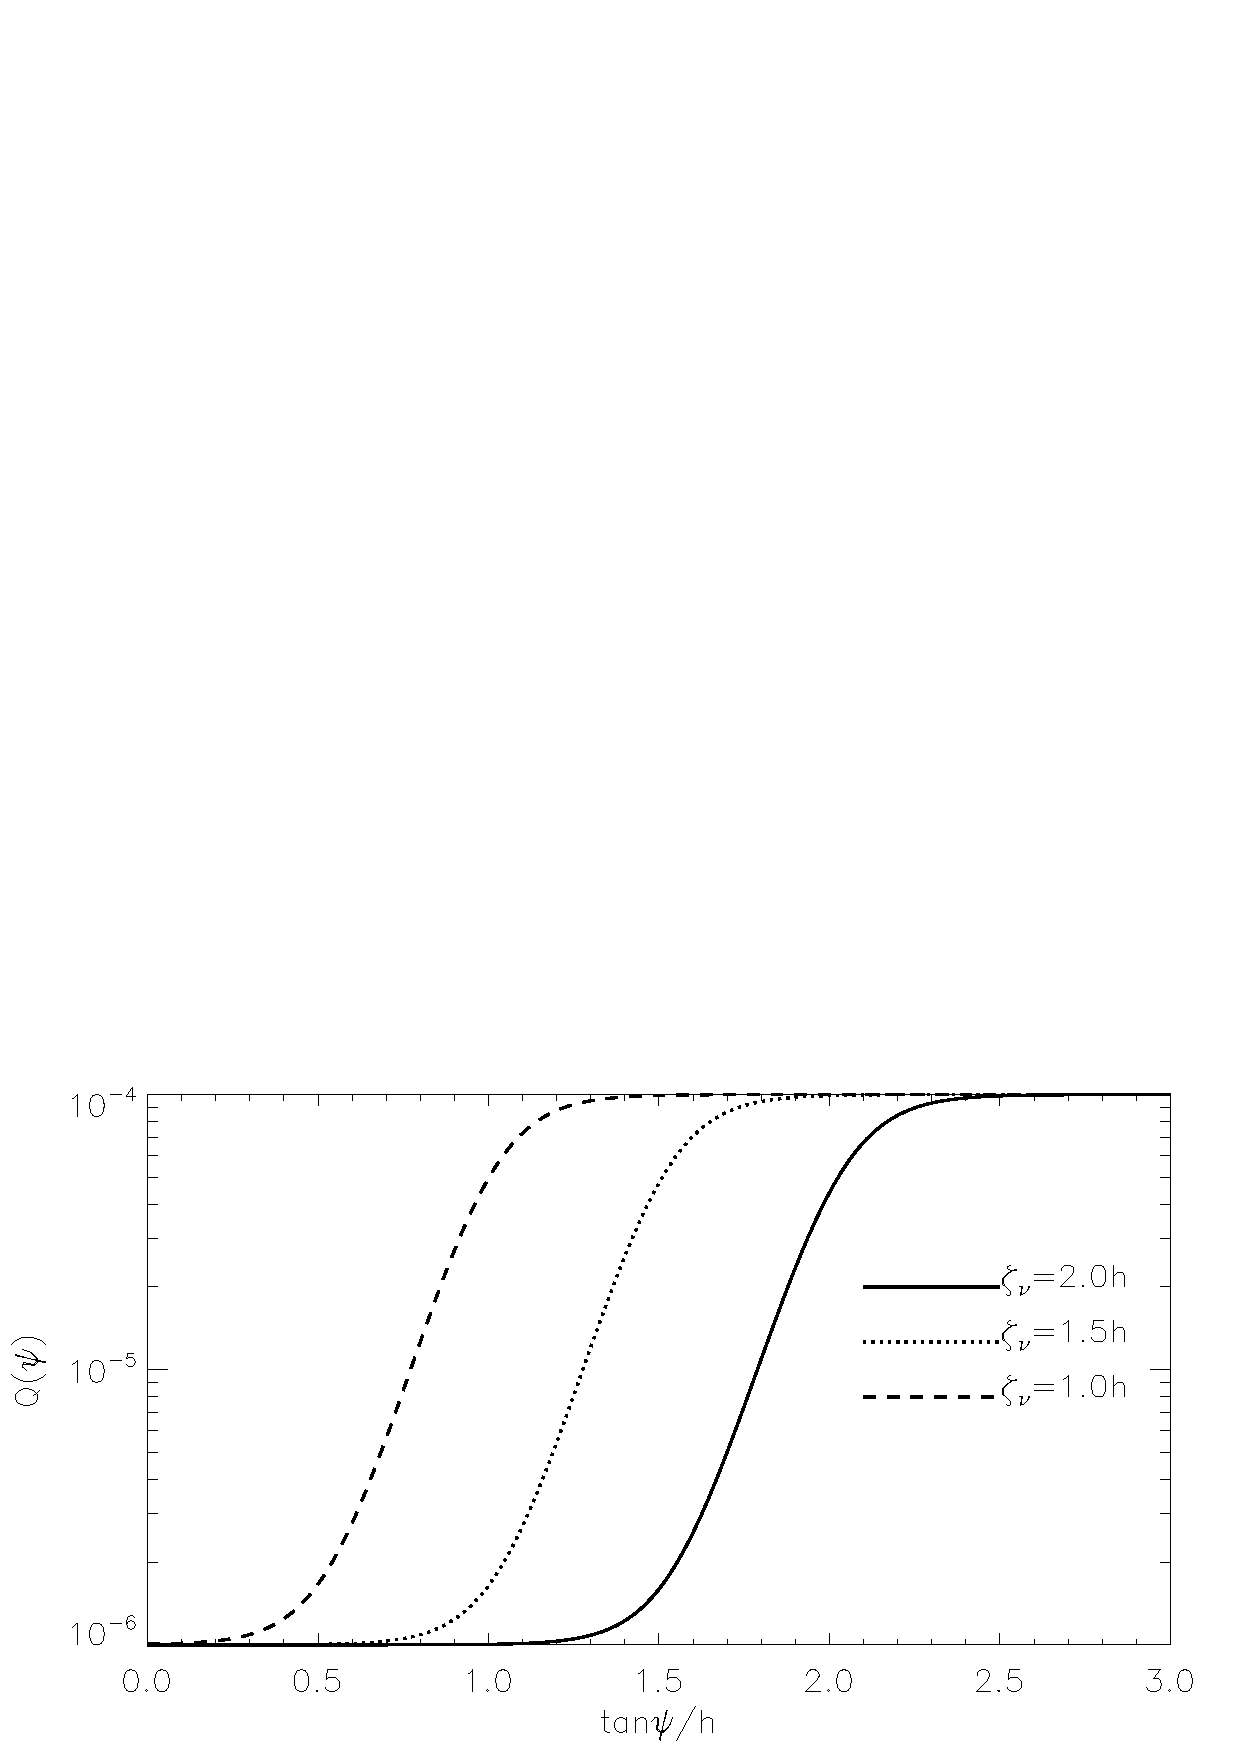
\includegraphics[width=\linewidth]{figures/pdisk_visc}
  \caption{Examples of the function $Q(\psi)$ 
    used in Eq. \ref{visc_profile} to increase
    the kinematic viscosity away from the midplane. The transition 
    occurs at $\psi = \zeta_\nu$, beyond which the kinematic viscosity
    is $A_\nu=100$ times larger than the midplane. All curves used
    $\Delta\zeta_\nu=0.2h$ for the transition width.
    \label{Qpsi}}
\end{figure}


\begin{figure}
  \centering
  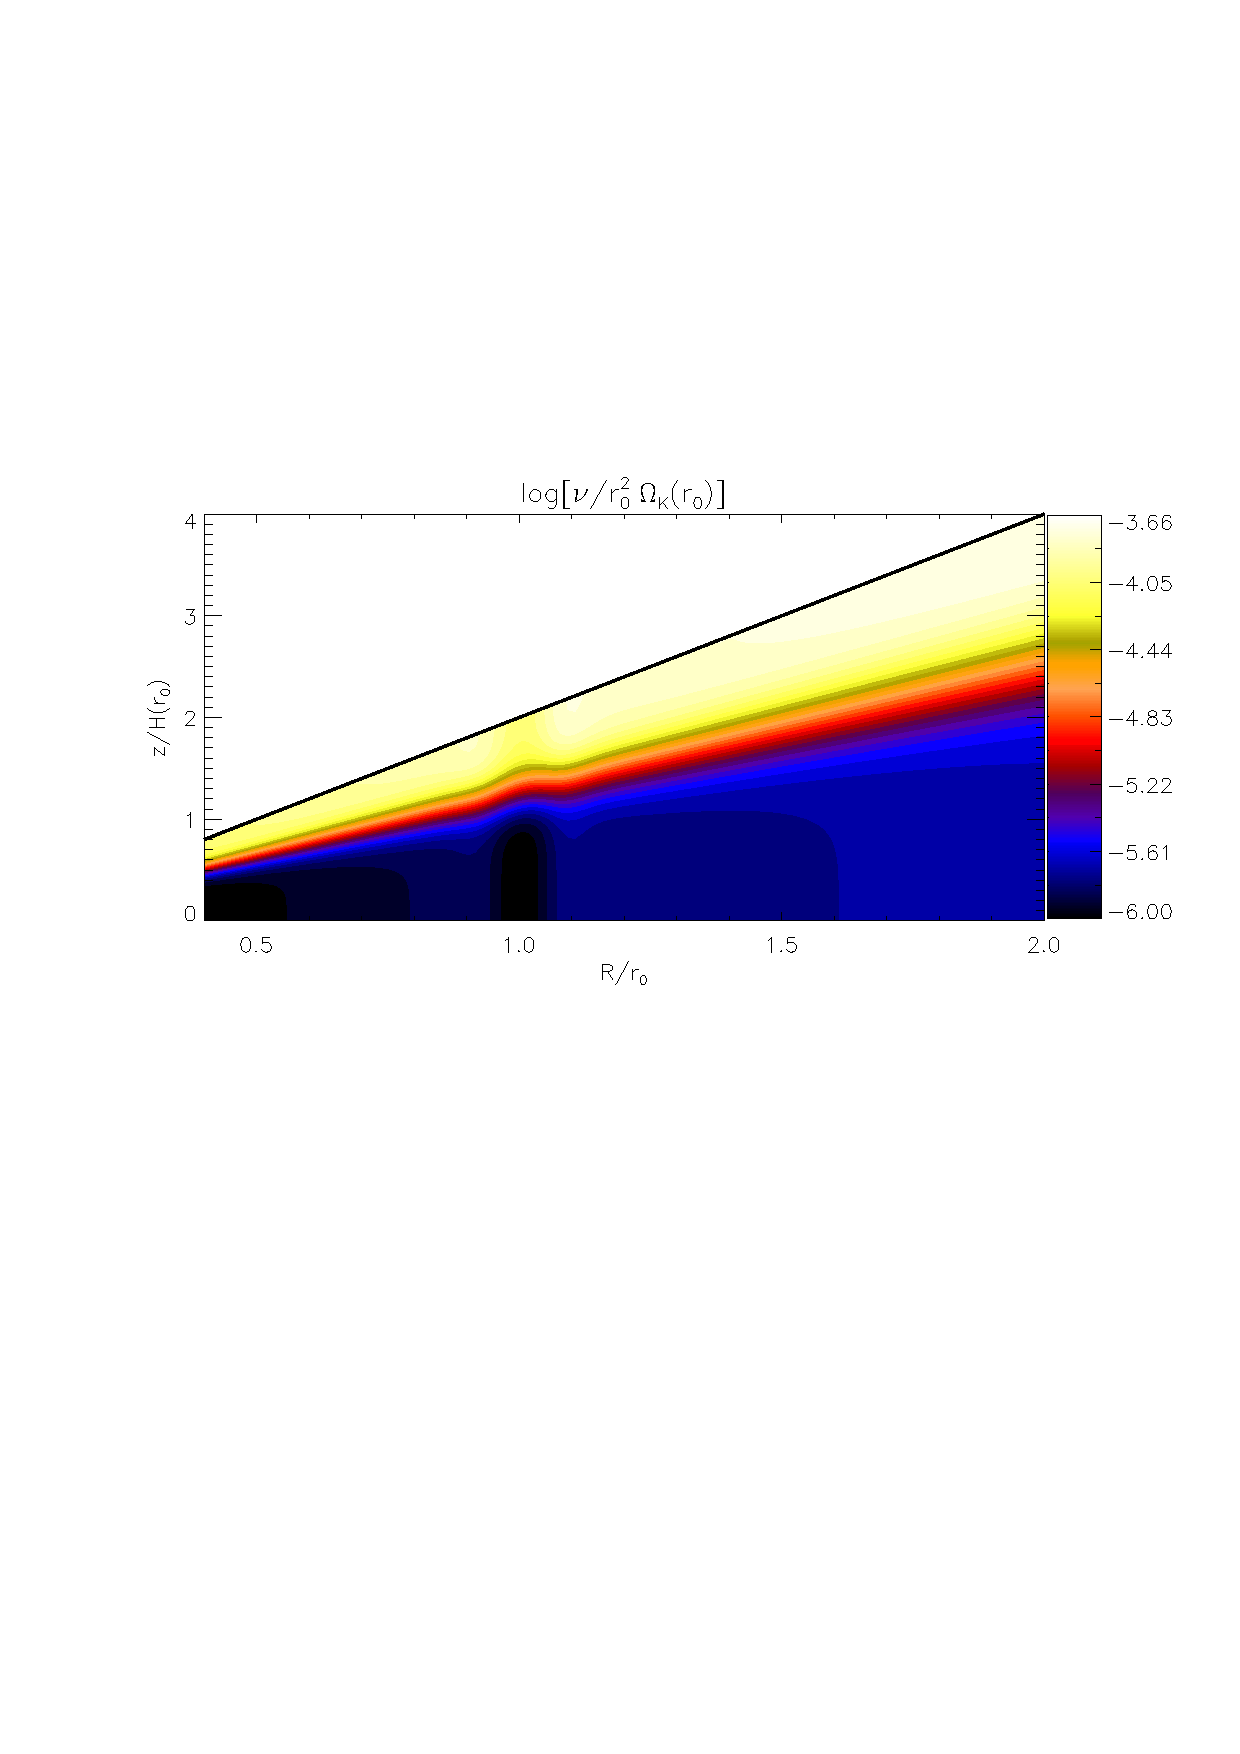
\includegraphics[width=\linewidth]{figures/pdisk_visc2d_2}
  \caption{Example of a two-layered kinematic viscosity profile
    resulting from Eq. \ref{visc_profile}. This specific plot
    corresponds to the numerical case V1, for which the solid line
    delineates the upper boundary of the computational domain.
    \label{visc2d}}
\end{figure}

\subsection{Artificial density bump}
We consider discs with aspect-ratio $h=0.1$ at unit radius, 
a radial extent of $[\rin,\rout]=[0.4,2.0]r_0$. The planetary
potential is disabled for these runs ($M_p\equiv 0$).  

The disc is initialized with $A=1.25$ and $\Delta R = 0.05r_0$ for the
bump parameters. The initial radial velocity is subject to random
perturbations of magnitude $10^{-4}c_s$. We employ $(N_r, N_\theta,
N_\phi)=(256,16n_h,512)$   
grid points, unless otherwise stated. 
(Recall $n_h$ parametrizes the vertical extent of the disc being
simulated.) The resolution at the reference radius is then $16$ cells
per $H$ in the meridional plane; and $8$ cells per $H$ in the azimuth. 

%% {\bf right now the resolution in r,phi is halved.}

\subsubsection{Inviscid runs}
Here we consider effectively inviscid discs by setting the viscosity
parameters $\hat{\nu}_0=10^{-9}$ and $A_\nu = 1$. The vertical extent
is $n_h=2$.     

Two simulations were run for with setup. Case B0 with a
reflective upper boundary and case B1 with an unperturbed upper
boundary. Setups similar to case B0 have previously been simulated both in the
linear and nonlinear regimes  \citep{meheut12, lin13}. So, in addition
to a control run, case B0 also serves to test the \pluto code in
simulating the RWI.  

\subsubsection{Viscous runs}
In these runs we explore the effect of viscous damping. In particular,
the influence of a viscous layer near the upper disc boundary. 
A reflective upper disc boundary condition is imposed.  

The control run for this setup is case V0 with: $\hat{\nu}_0=10^{-6}$,
$n_h=2$ and $A_\nu = 1$. Thus, case V0 is the viscous version of case 
B0. We then consider models where the kinematic viscosity increases by
a factor $A_\nu=100$ beyond $\psi=\zeta_\nu$. The angular transition
width is fixed to $\Delta\zeta_\nu=0.2h$. In the first instance, we
maintain a vertical domain size of $n_h=2$, and choose
$\zeta_\nu=1.5h,\,1.0h$ for cases V1 and V2, respectively. This gives a
viscous layer of thickness $0.5H$ and $H$ near the upper boundary at
the reference radius. (See Fig. \ref{visc2d} for a plot of the
kinematic viscosity profile for case V1.) Finally, we consider a high
viscosity run, case V3, with $\hat{\nu}_0=10^{-4}$ and $A_\nu=1$. Case
V3 is equivalent to increasing the viscous layer of case V2 to occupy
the entire vertical domain, i.e. setting $\zeta_\nu\to 0$.
 
We also consider appending an upper viscous layer to the control
case. Case V0e has vertical extent $n_h=3$ and transition height
$\psi_\nu=0.2$. 




































Table \ref{artificial_bump} lists the setups for simulations 
initialized with a density bump, along with several diagnostic measures 
of each case. The disc evolution is divided into two stages. The first
being $t\leq 10P_0$ when relative density perturbations are small 
($\delta\rho\ll 1$). For convenience we will refer 
to this stage as the `linear phase'. The dominant azimuthal wavenumber
is the fastest growing linear mode. Mode frequencies are averaged over
the shell $r\in[0.8,1.2]r_0$, and time-averaged over $t\in[5,10]P_0$.    

The second set of measurements is made well into the non-linear
regime, at $t=100P_0$. The dominant mode is that with
$\mathrm{max}[a_m(100P_0)]$. The minimum Rossby number is measured at
the midplane. 
%%  The alpha paramete quoted in Table
%% \ref{artificial_bump}, which is measured at the midplane, has been
%% averaged over $R\in[0.8,1.2]r_0$ and $t\in[0,100]P_0$. 

\begin{table*}
  \centering
  \caption{Summary of hydrodynamic simulations initialized with a
    density bump. `UBC' is
  the condition applied at the upper disc boundary. \label{artificial_bump}}
 \begin{tabular}{lllcccccl @{\extracolsep{0.1cm}} ccc}
    \hline\hline
    \multicolumn{6}{c}{\phantom{stuff}} &
    \multicolumn{3}{c}{Linear phase ($t\leq10P_0$)}&
    \multicolumn{3}{c}{$t=100P_0$}\\
    \cline{7-9}\cline{10-12}
    Case & UBC & $n_h$ & $\log{\hat{\nu}_0}$ & $A_\nu$ &$\zeta_\nu/h$ & $m$ &
    $\overline{\omega_m}/\Omega_0$ &
    $\overline{q_m}/\Omega_0$ &  
    $m$ & $10^2a_m$ & $\mathrm{min}[Ro(z=0)]$ \\ 
    \hline
    B0 & reflec. & 2 &-9 & 1 &n/a & 4 & 0.984 & 0.201 %omit = 3
    & 1  & 8.5  &  -0.15  \\  
    B1 & unpert. & 2 &-9 & 1 &n/a & 4  & 0.985 & 0.191 
    & 1 &  2.2 &   -0.10 \\
    V0 & reflec. & 2 &-6 & 1 &n/a & 4  & 0.984 & 0.201   
    & 1 & 7.0 &   -0.11 \\
    V0e & reflec. & 3 &-6 & 100 &  2.0 & 4   &  0.983   &  0.189 
    & 1 & 7.4 &   -0.18 \\
    V1 & reflec. & 2 &-6 & 100 & 1.5  & 4 & 0.983  & 0.188  
    & 1  & 6.2 &  -0.22 \\
    V2 & reflec. & 2 & -6 & 100 & 1.0  & 4   &  0.982 & 0.176  
    & 2  & 5.5 &   -0.22\\
    V3 & reflec. & 2 & -4 & 1 & n/a  &   4 & 0.984  & 0.129  
    & 3  & 3.3   &  -0.27 \\
   \hline
  \end{tabular}
\end{table*}


\subsection{Reflective verses unperturbed upper boundary}
We first demonstrate the impact of numerical boundary conditions. 
Fig. \ref{bump0_bump1}--- \ref{bump0_bump1_vort} compares case B0 
with a reflective upper boundary, and case B1 which imposes an
unperturbed boundary. The non-axisymmetric density field and Rossby
numbers are shown. The evolution for case B0 is fairly typical, and
has been described in detailed in other studies
\citep[e.g.][]{meheut12}. The $m=4$ linear mode is dominant at early
times, implying the formation of 4 vortices initially. They
subsequently merge into a single vortex on a dynamical time-scale. 

%why not find this linear mode in linear calc? 

In the linear regime case B1 is similar to case B0. The most 
unstable linear mode growth rate decreases by about $5\%$  (Table
\ref{artificial_bump}). However, the non-linear evolution of case B1
differs significantly from case B0. The final non-axisymmetry is weak
, $|\Delta\rho|\sim 6\%$ (c.f. $\sim 50\%$ for case B0), and there is
no distinct vortical structure. Vortex formation has been suppressed
by changing the numerical boundary conditions. 

It is clear from this simple experiment that vortex formation through
the RWI is an intrinsically global process in the vertical direction, 
so it can be significantly influenced by vertical boundary conditions.  

 \begin{figure}
   \centering
   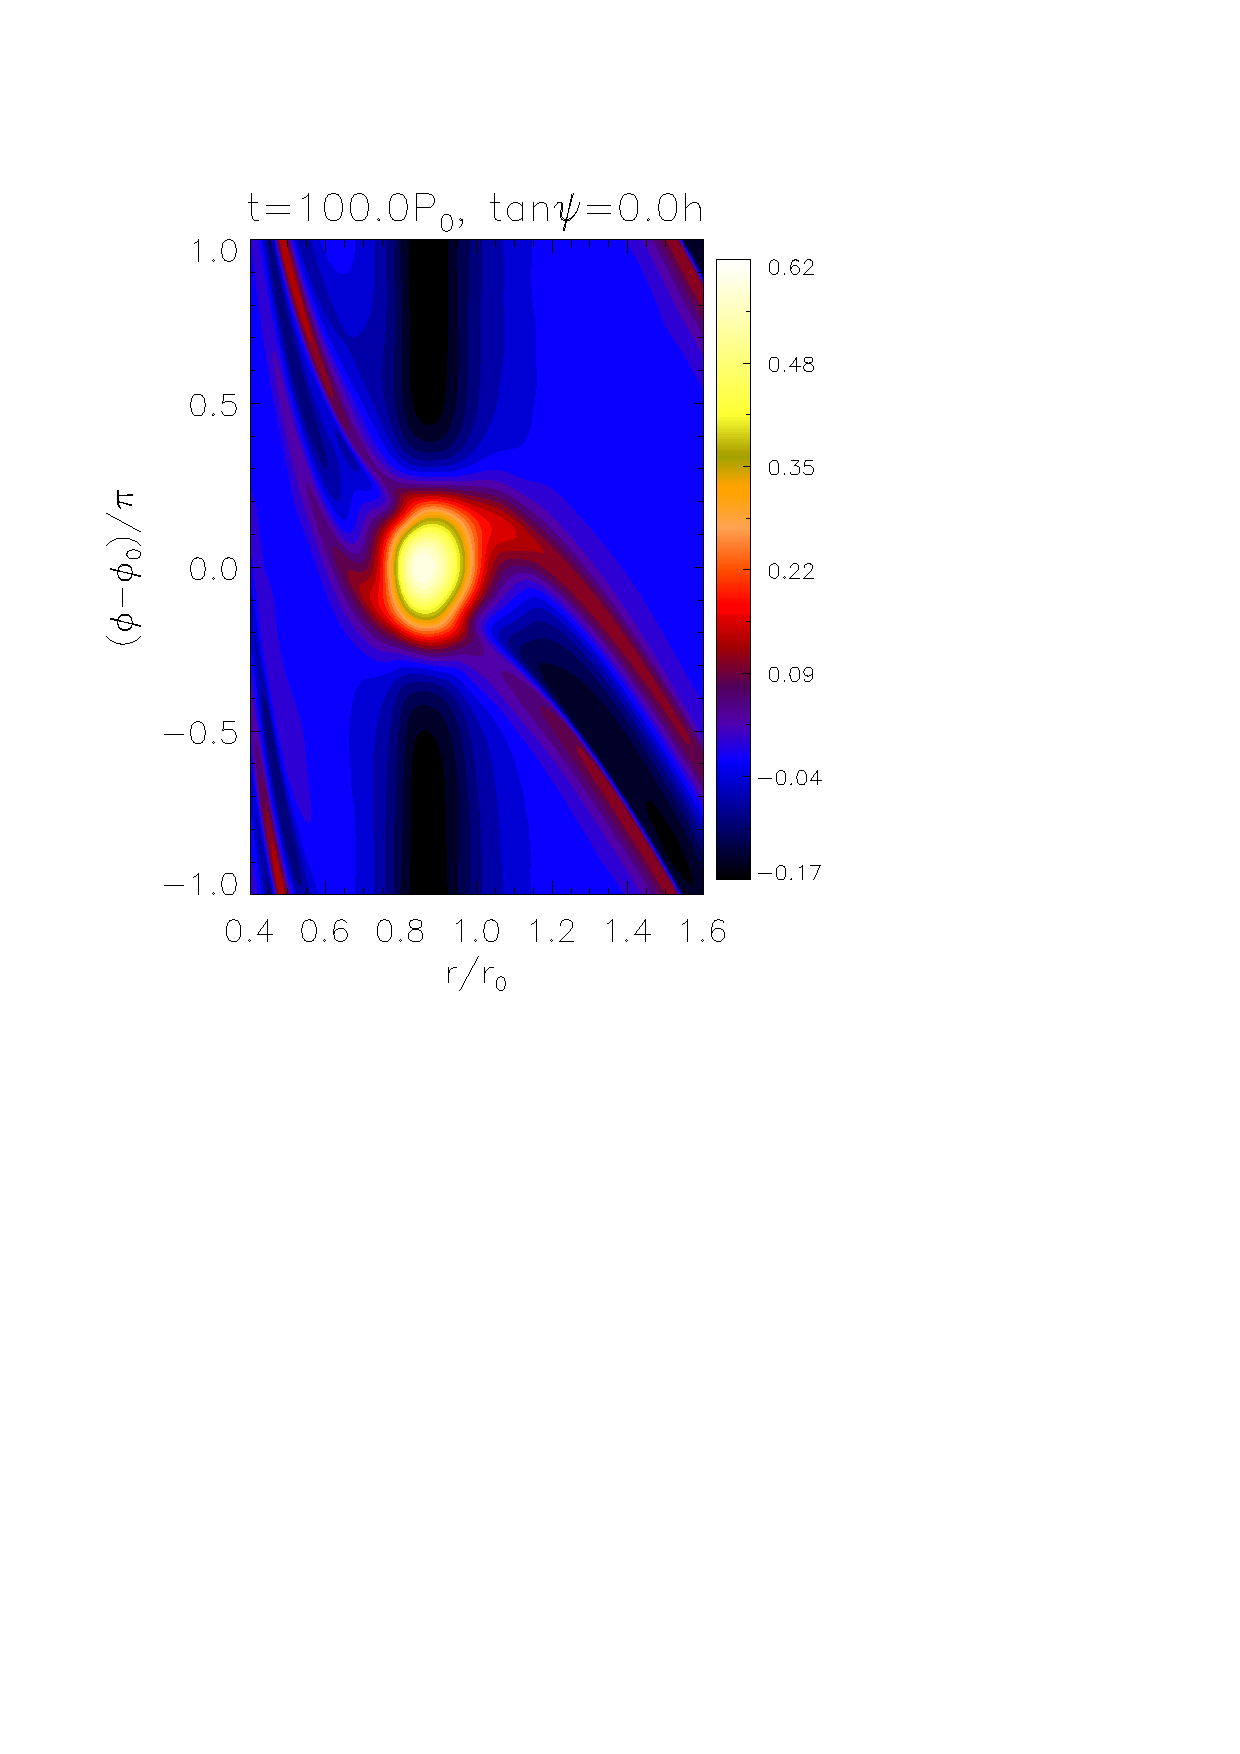
\includegraphics[scale=.27,clip=true,trim=0cm 1.84cm 0cm
     0cm]{figures/bump0_pdisk010}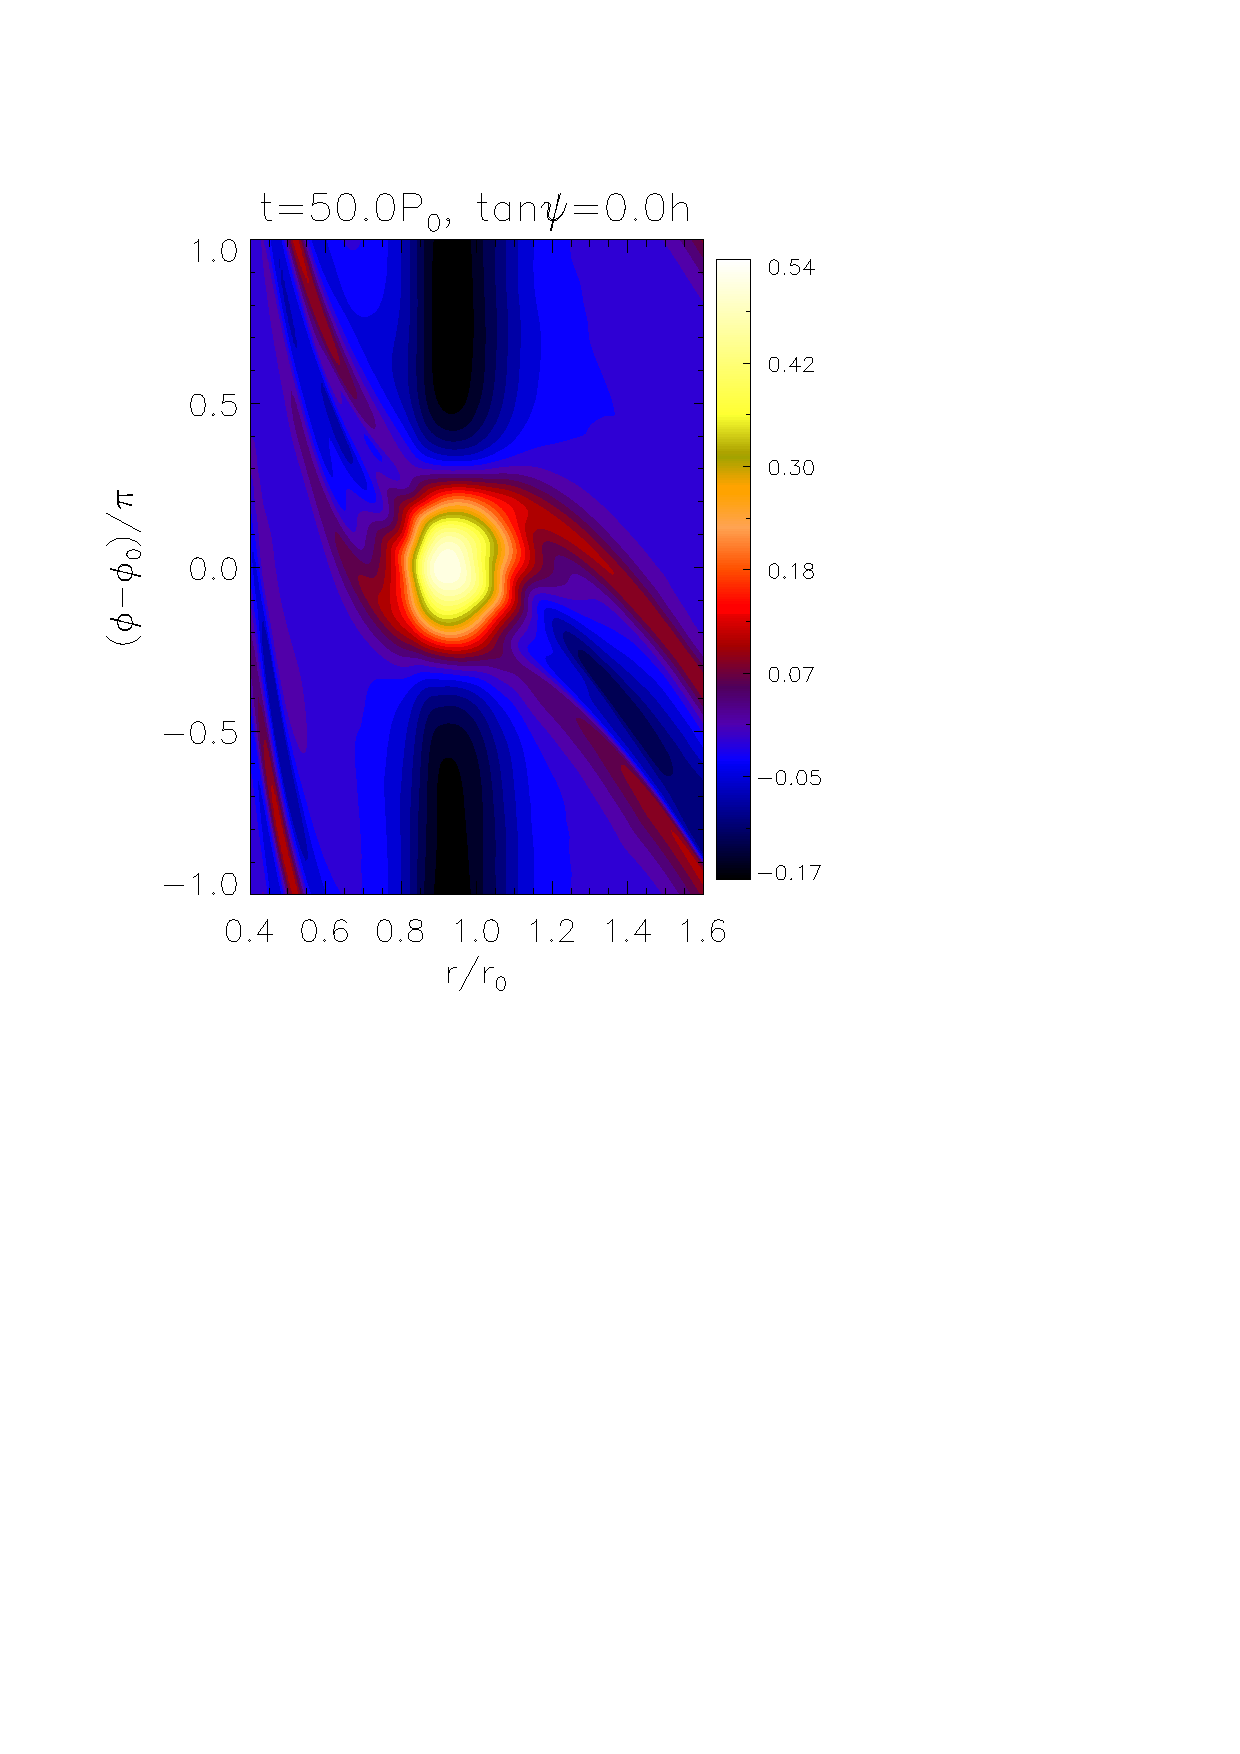
\includegraphics[scale=.27,clip=true,trim=2.3cm
     1.84cm 0cm
     0cm]{figures/bump0_pdisk014}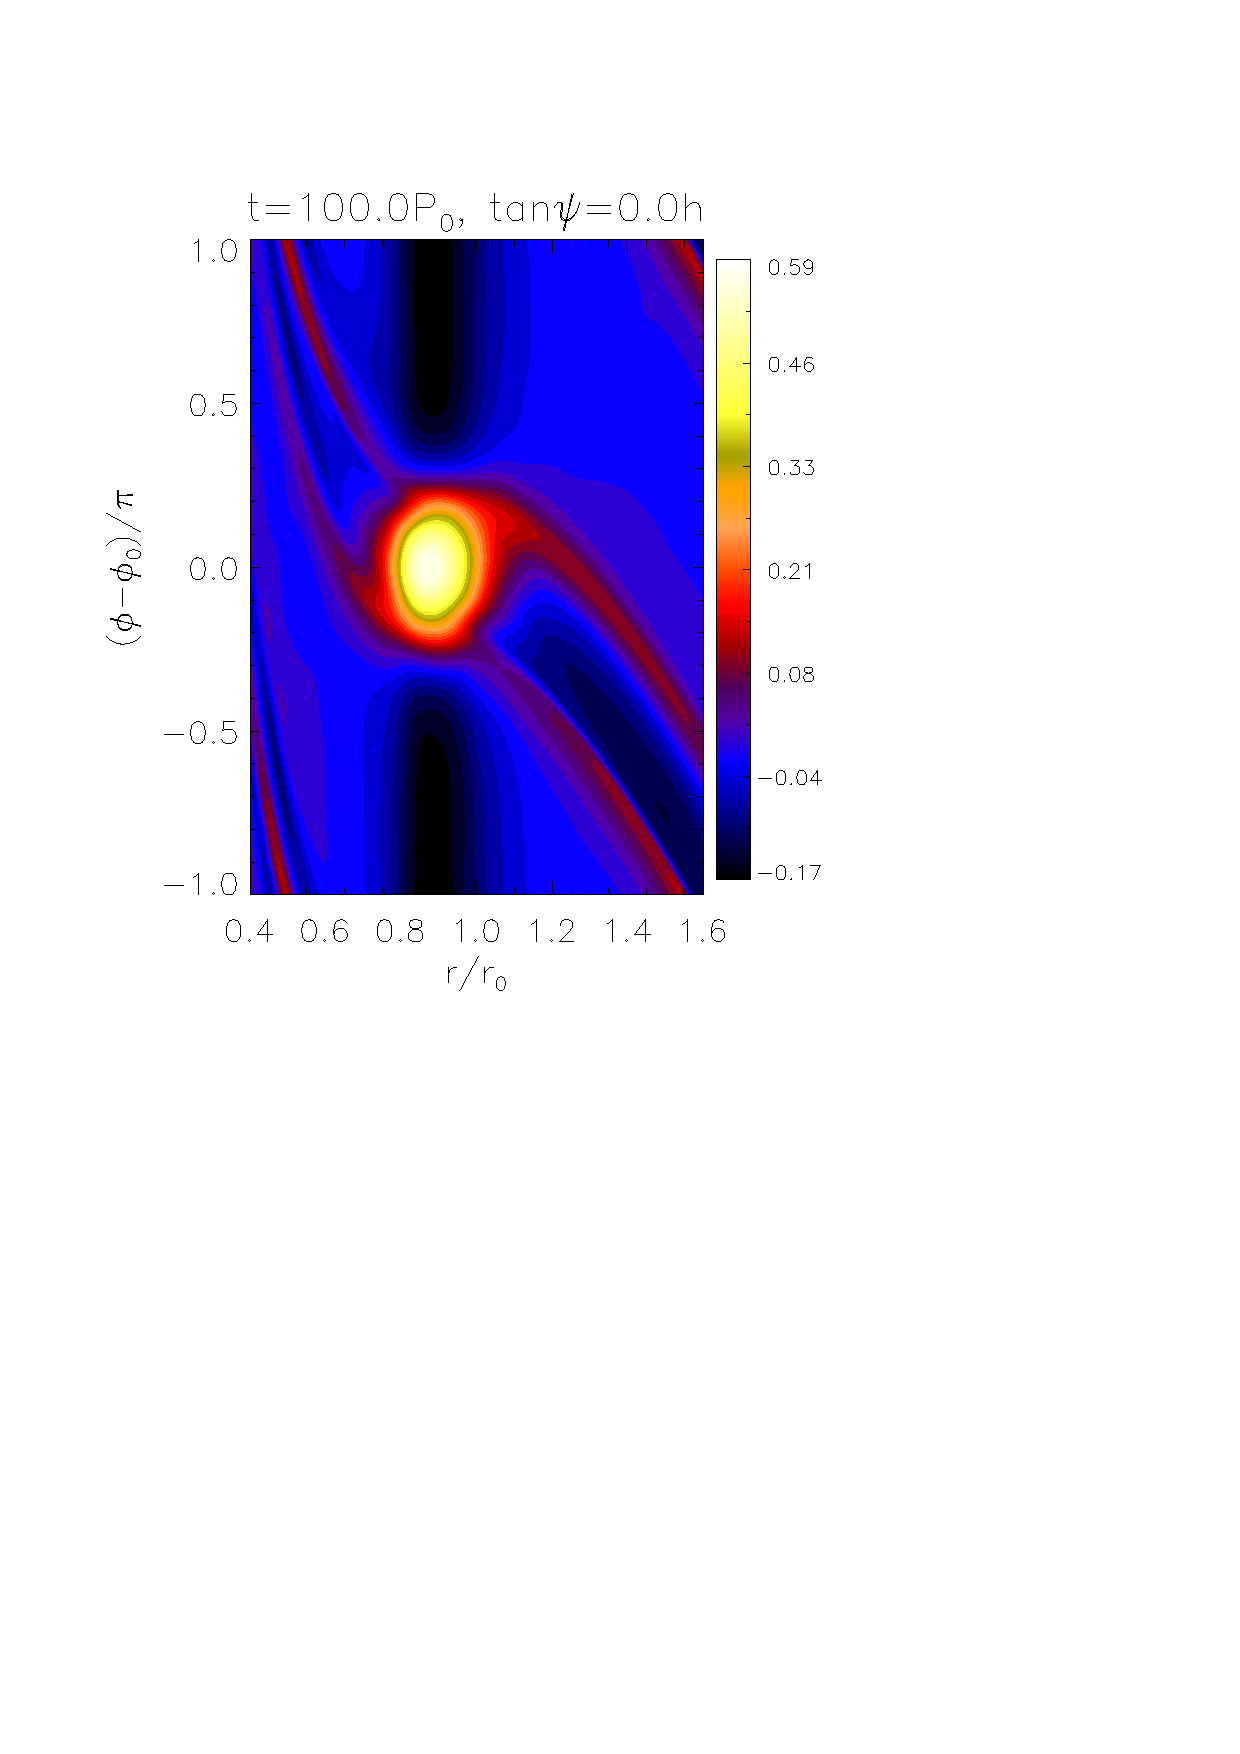
\includegraphics[scale=.27,clip=true,clip=true,trim=2.3cm
     1.84cm 0cm
     0cm]{figures/bump0_pdisk019}\\
   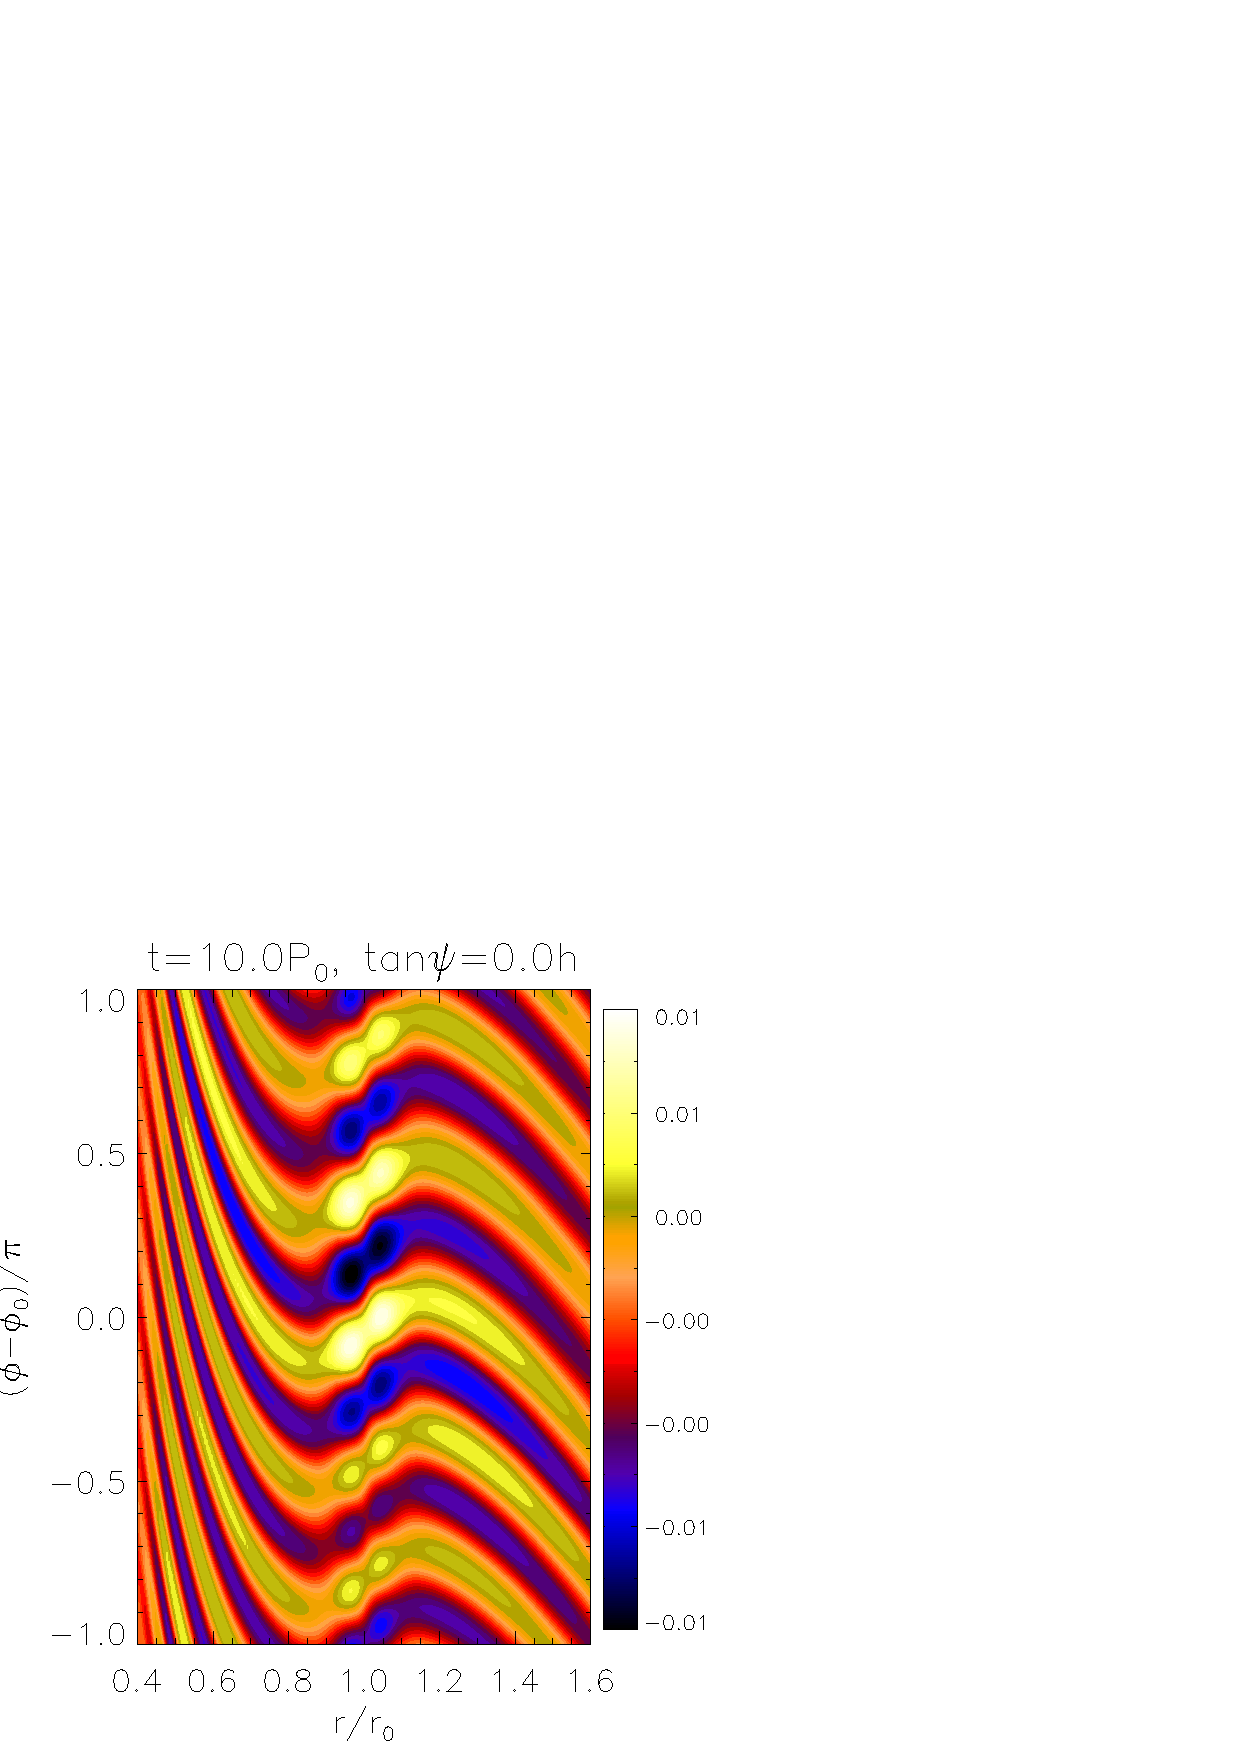
\includegraphics[scale=.27,clip=true,trim=0cm 0.cm 0.0cm
     0.99cm]{figures/bump1_pdisk010}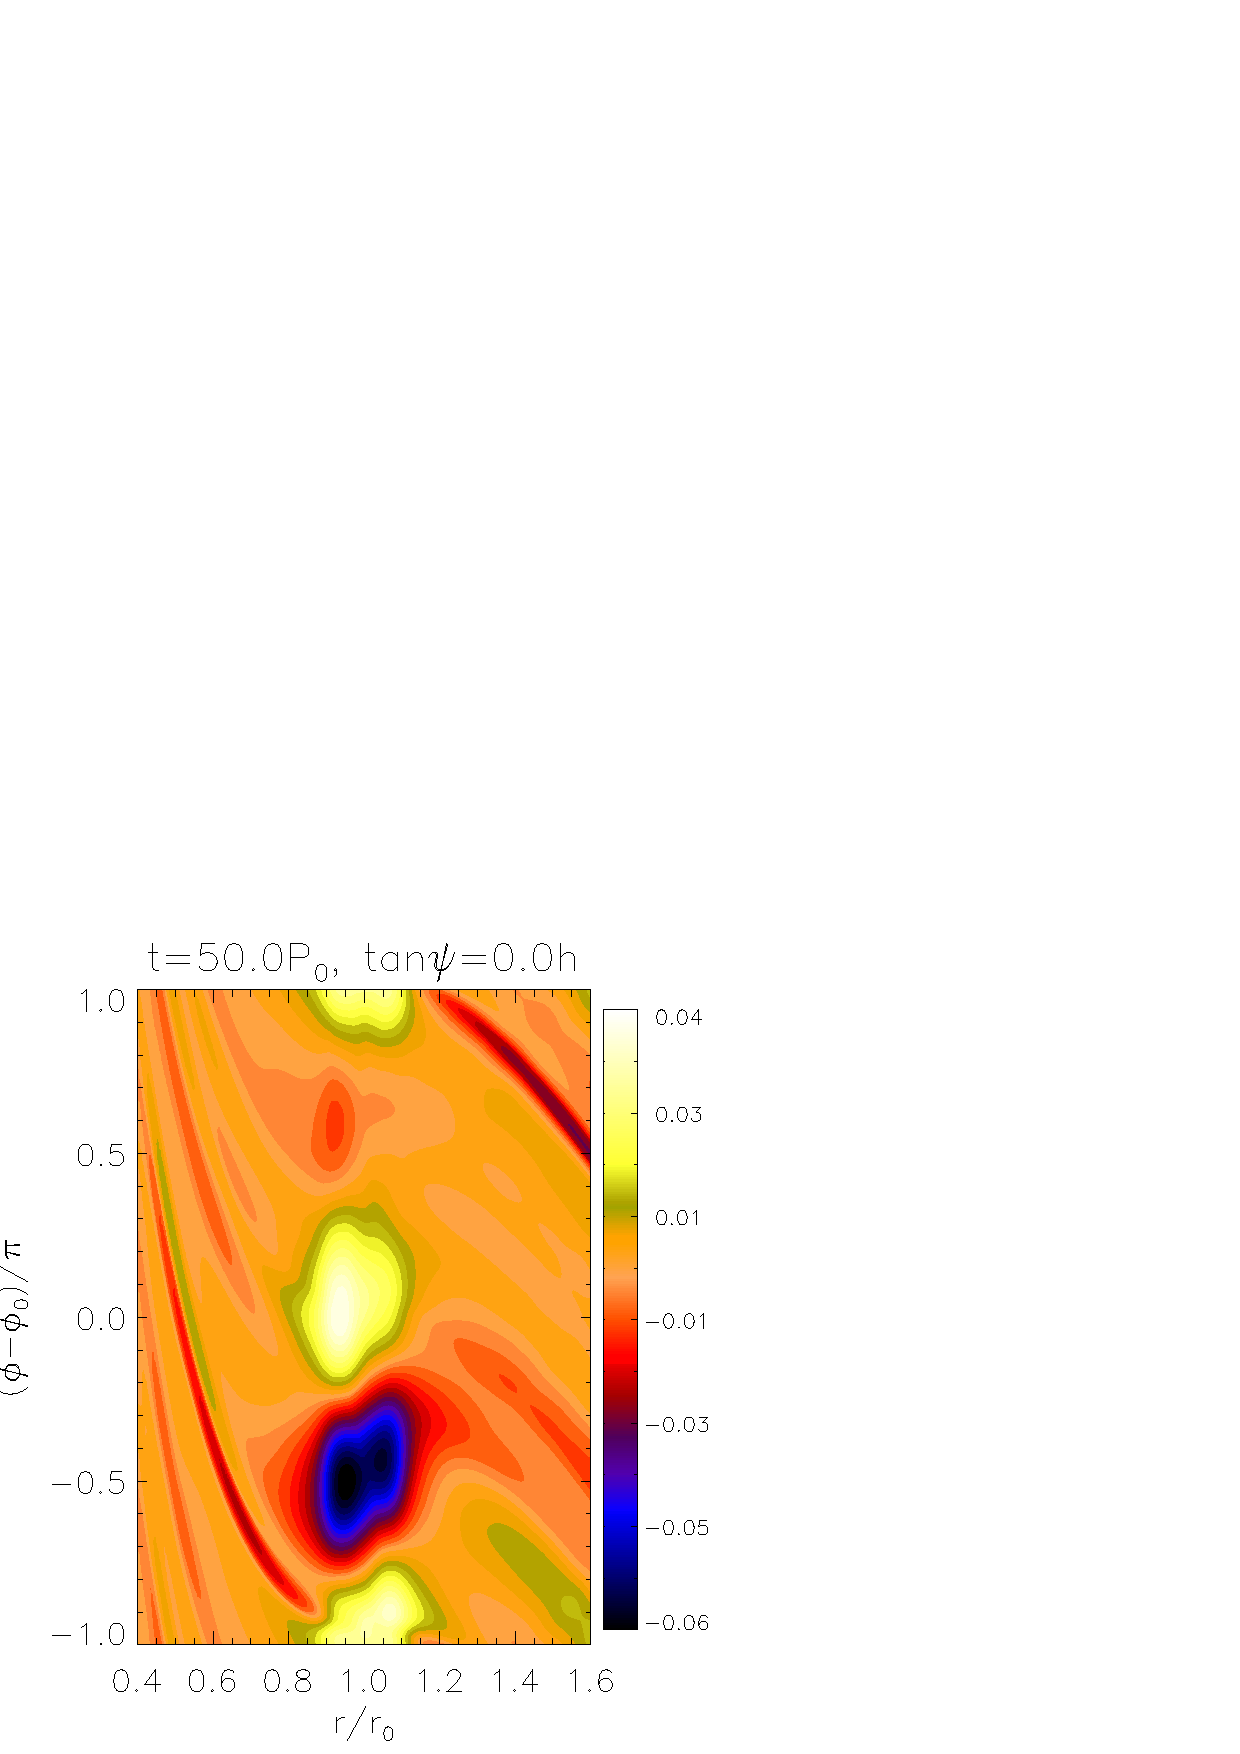
\includegraphics[scale=.27,clip=true,trim=2.3cm
     0.cm 0.cm
     0.99cm]{figures/bump1_pdisk014}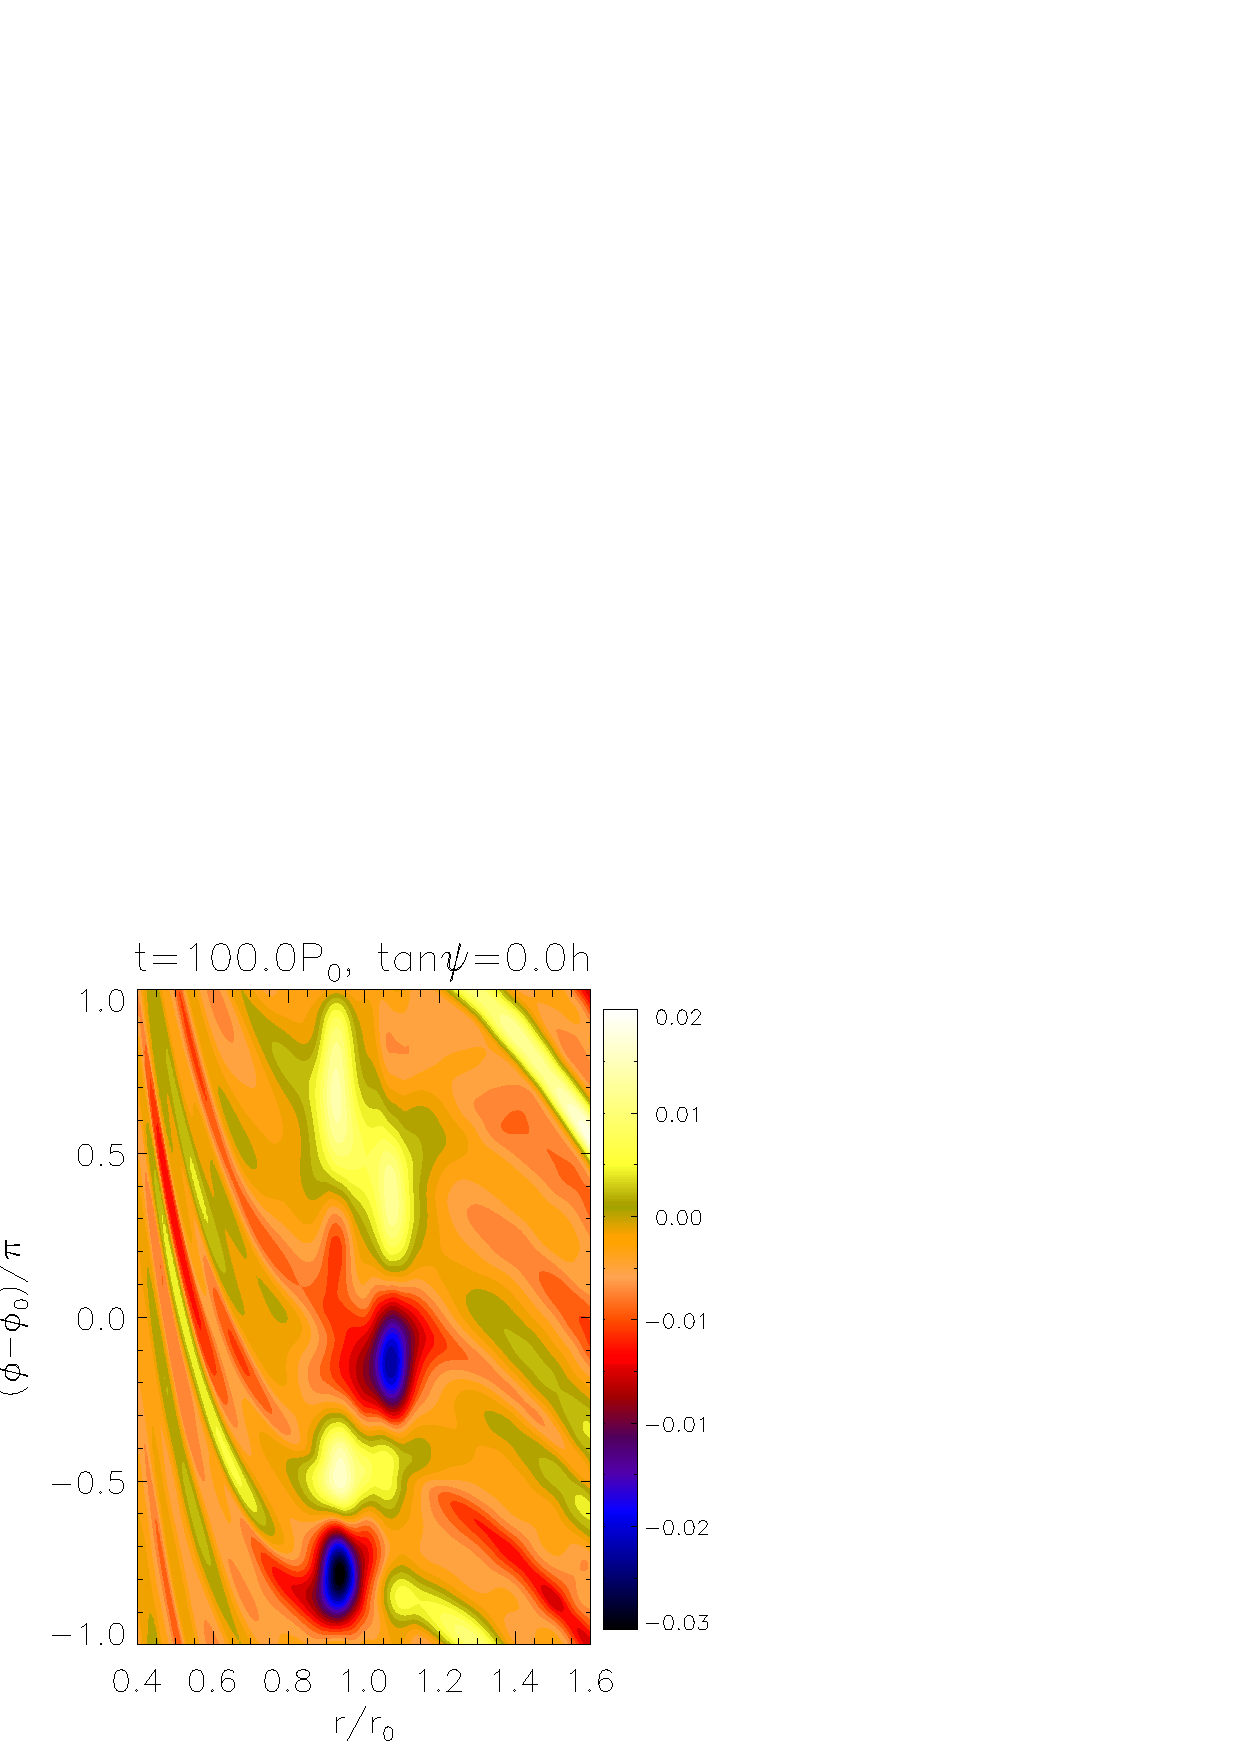
\includegraphics[scale=.27,clip=true,clip=true,trim=2.3cm
     0.cm 0.cm
     0.99cm]{figures/bump1_pdisk019}  
   \caption{Evolution of the midplane non-axisymmetric density field,
     $\Delta\rho(z=0)$, for case B0 with a reflective upper boundary
     (top) and case  
     B1  with an unperturbed upper boundary (bottom). $\phi_0$ is the
     azimuth of $\mathrm{max}(|\Delta\rho(z=0)|)$.   
   \label{bump0_bump1}}
 \end{figure}

\begin{figure}
   \centering
   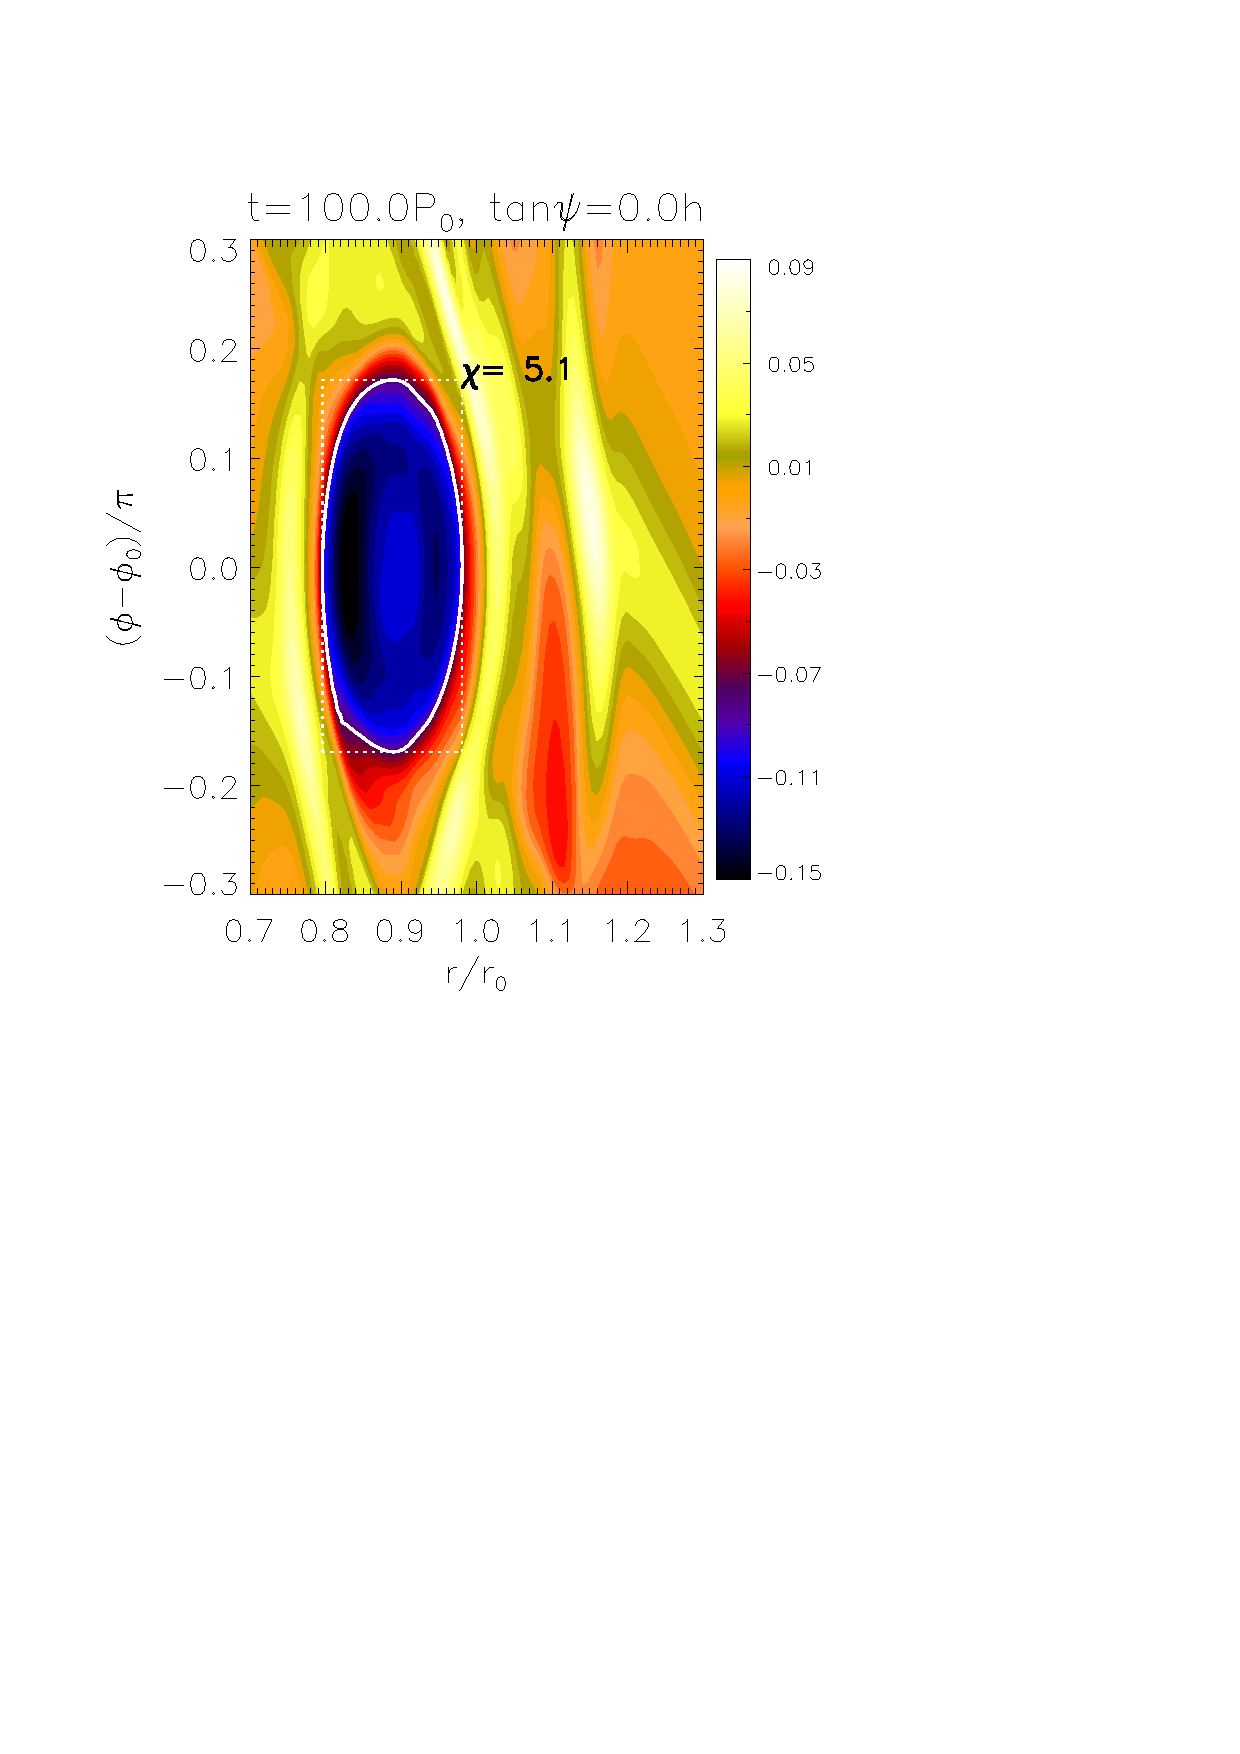
\includegraphics[scale=.27,clip=true,trim=0cm 1.84cm 0cm
     0cm]{figures/bump0_vort010}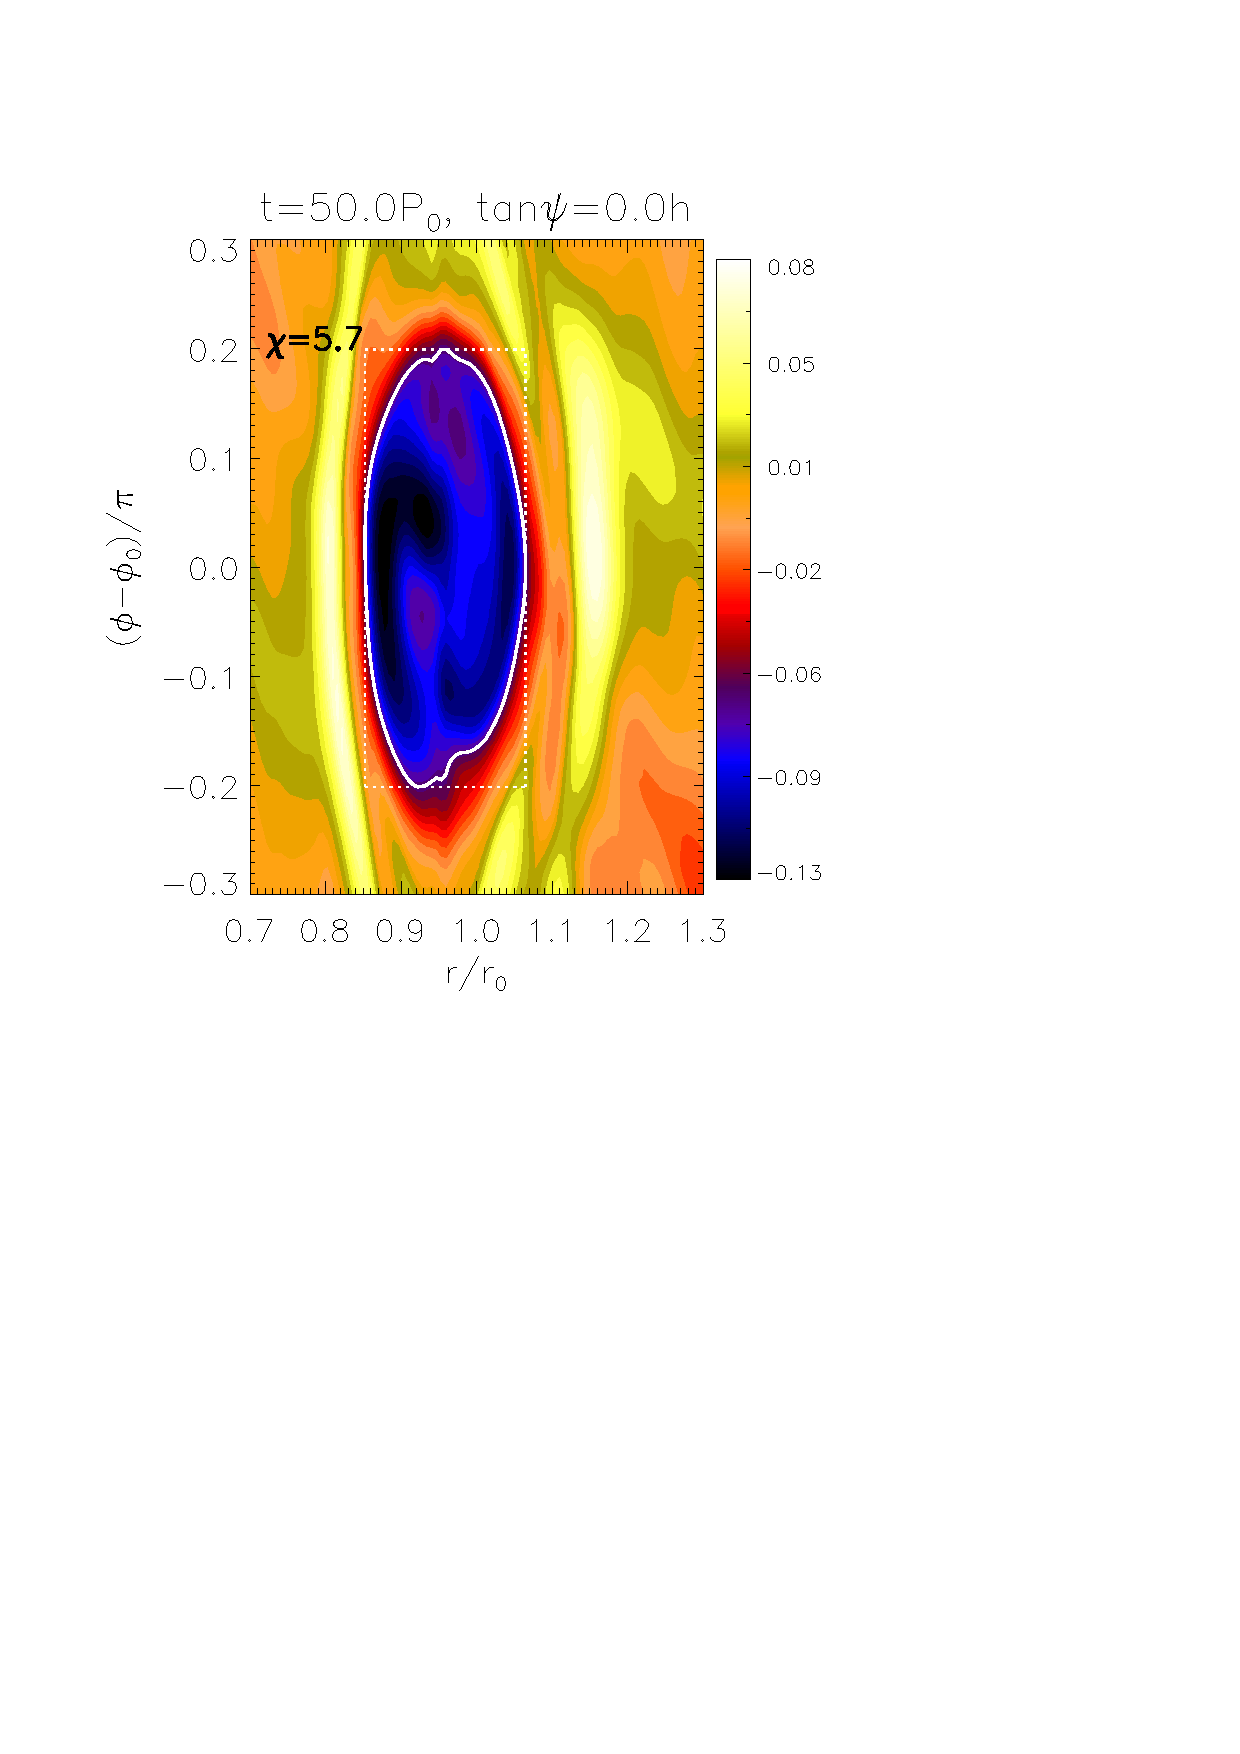
\includegraphics[scale=.27,clip=true,trim=2.3cm
     1.84cm 0cm
     0cm]{figures/bump0_vort014}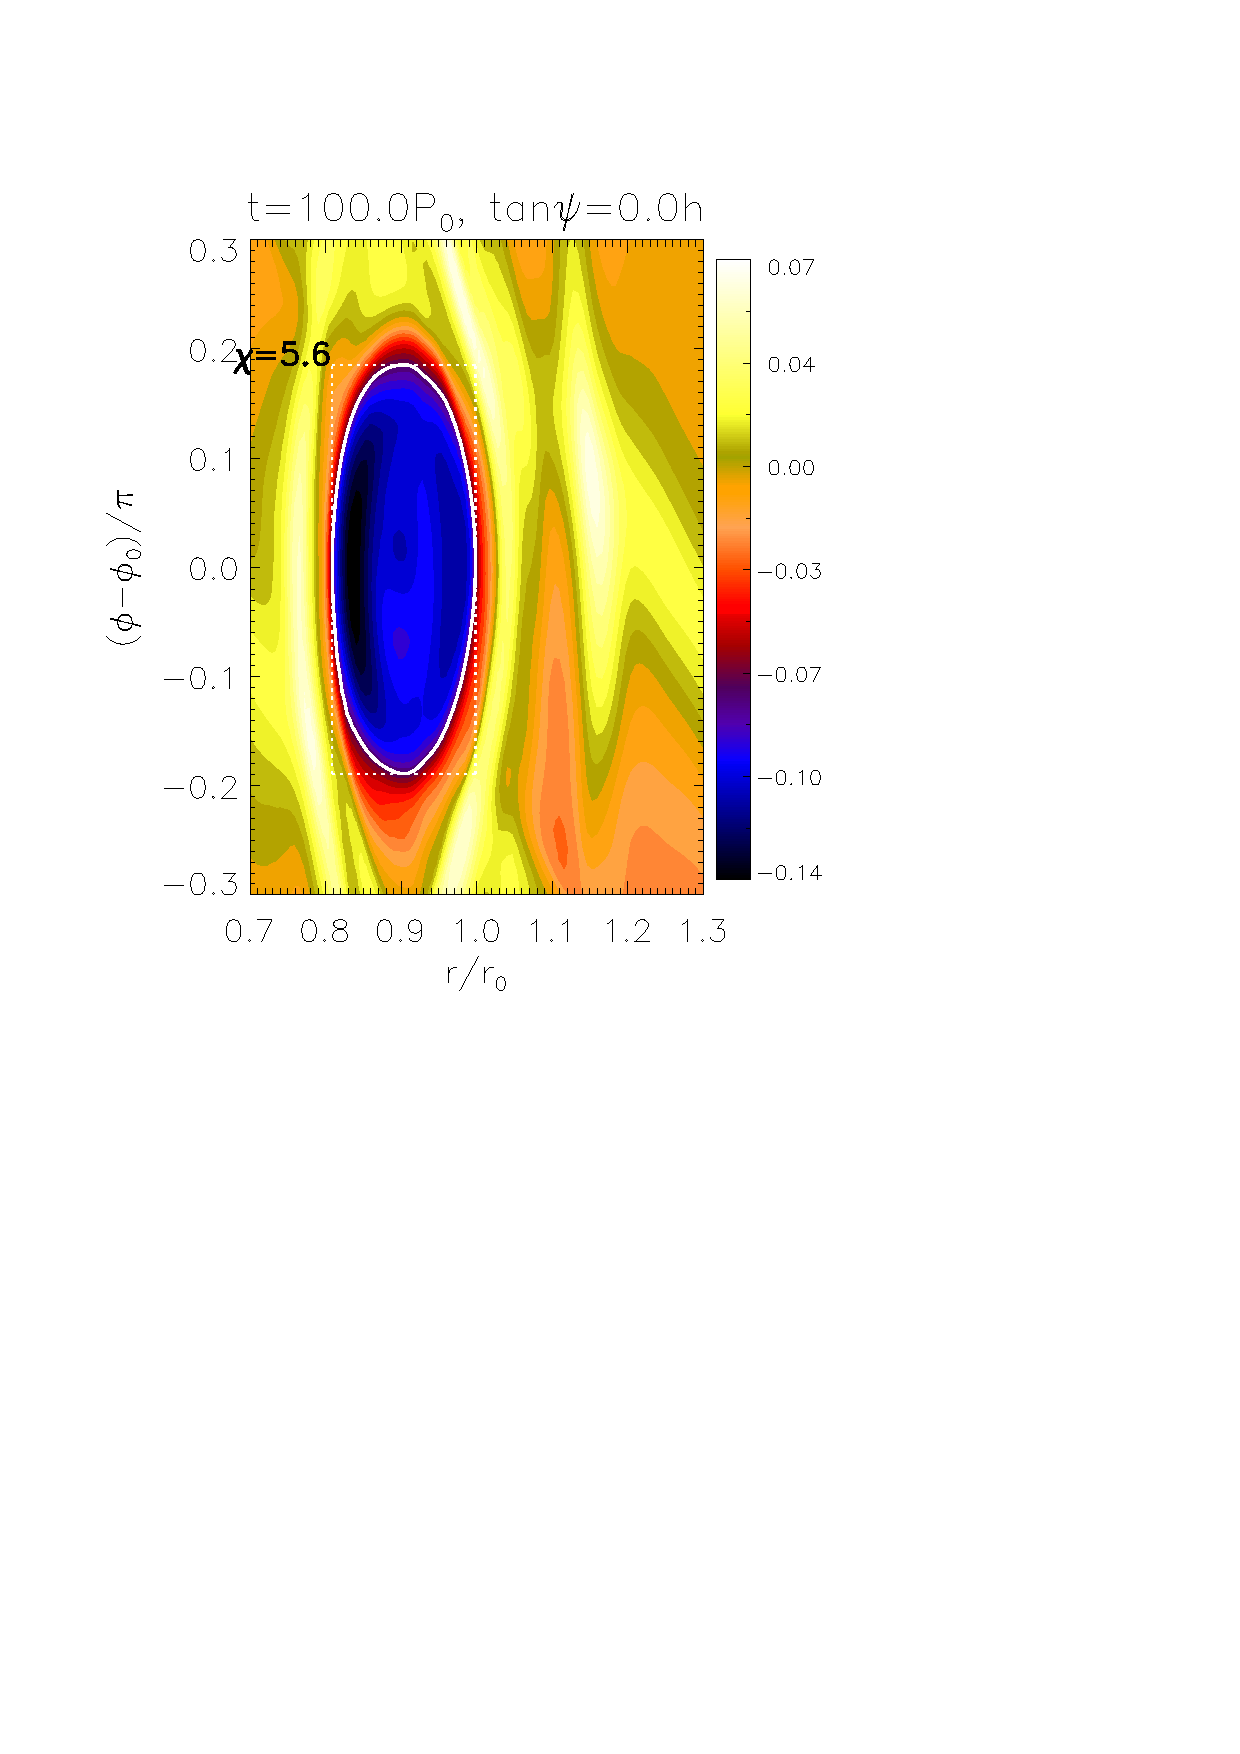
\includegraphics[scale=.27,clip=true,clip=true,trim=2.3cm
     1.84cm 0cm
     0cm]{figures/bump0_vort019}\\
   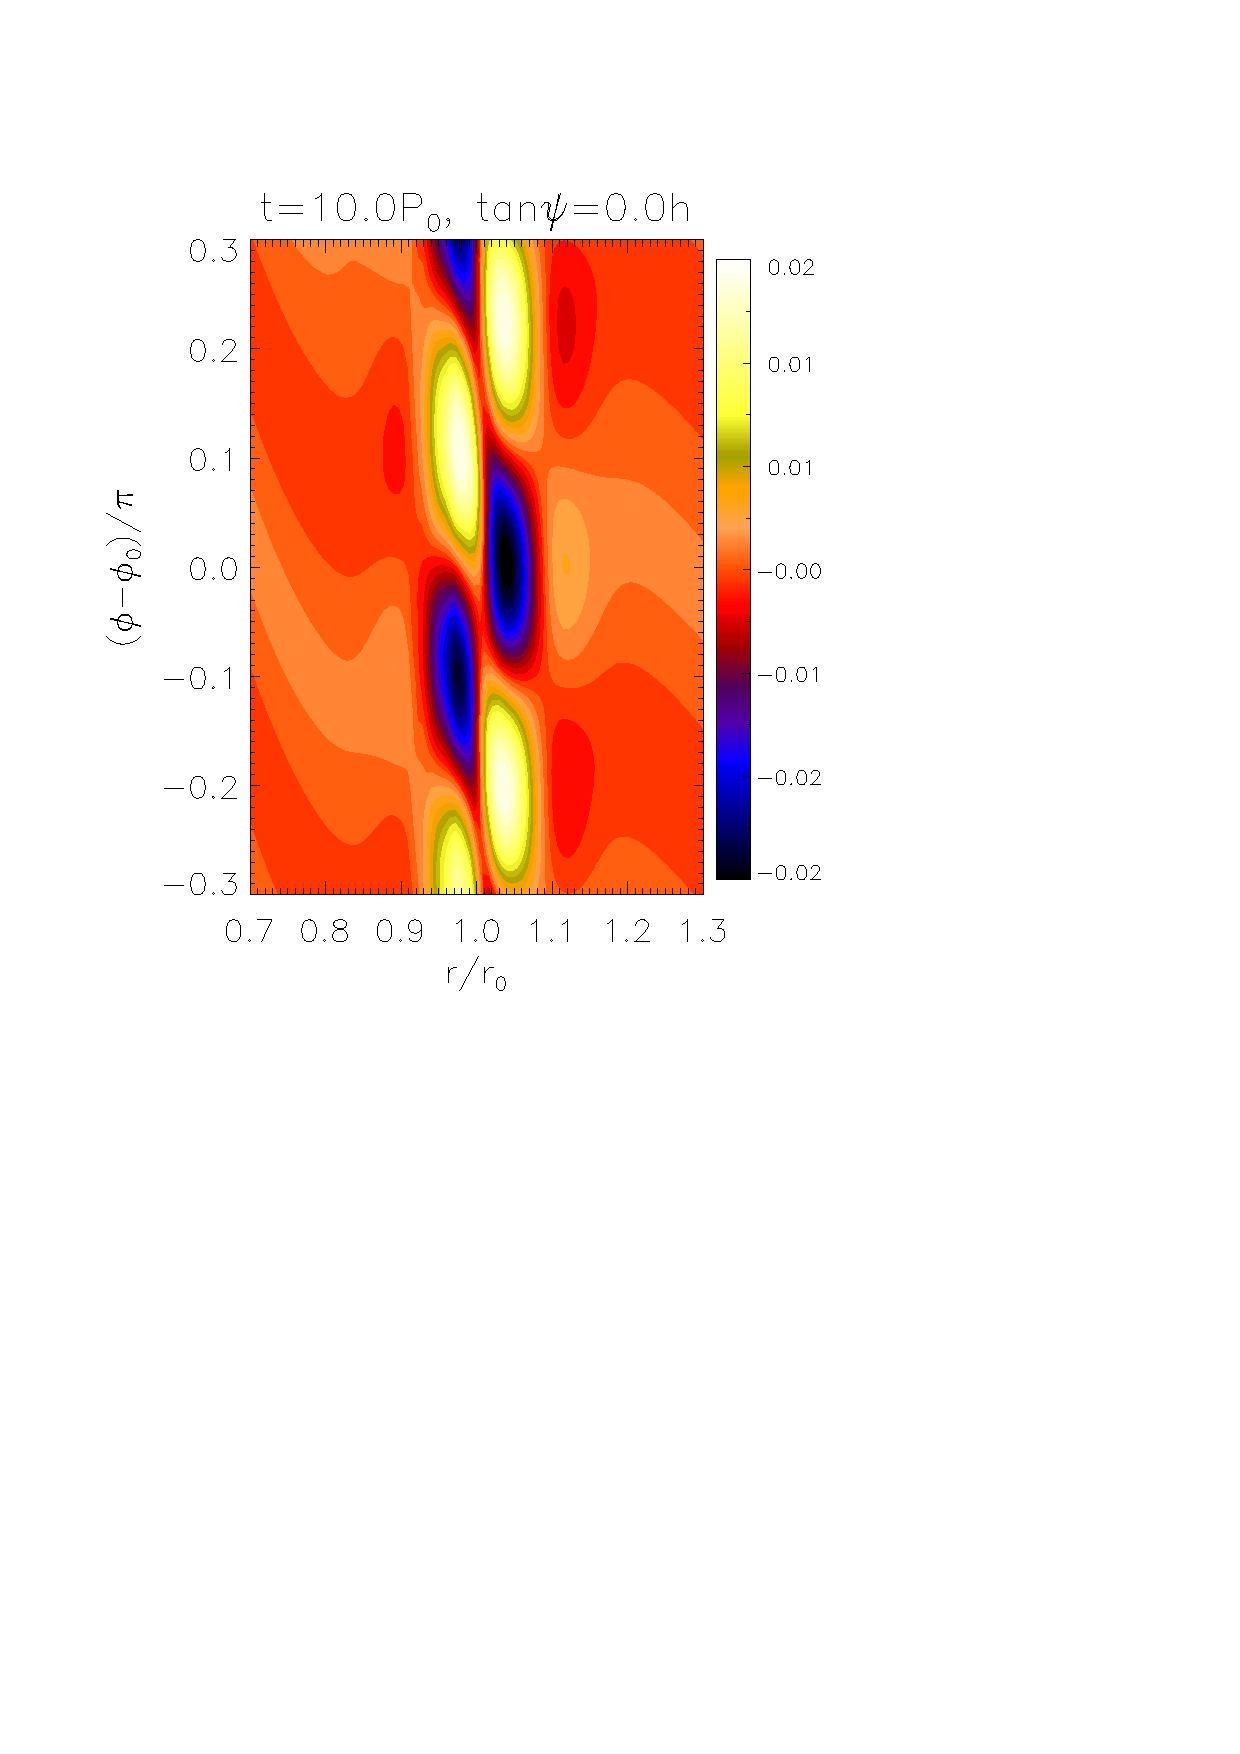
\includegraphics[scale=.27,clip=true,trim=0cm 0.cm 0.0cm
     0.99cm]{figures/bump1_vort010}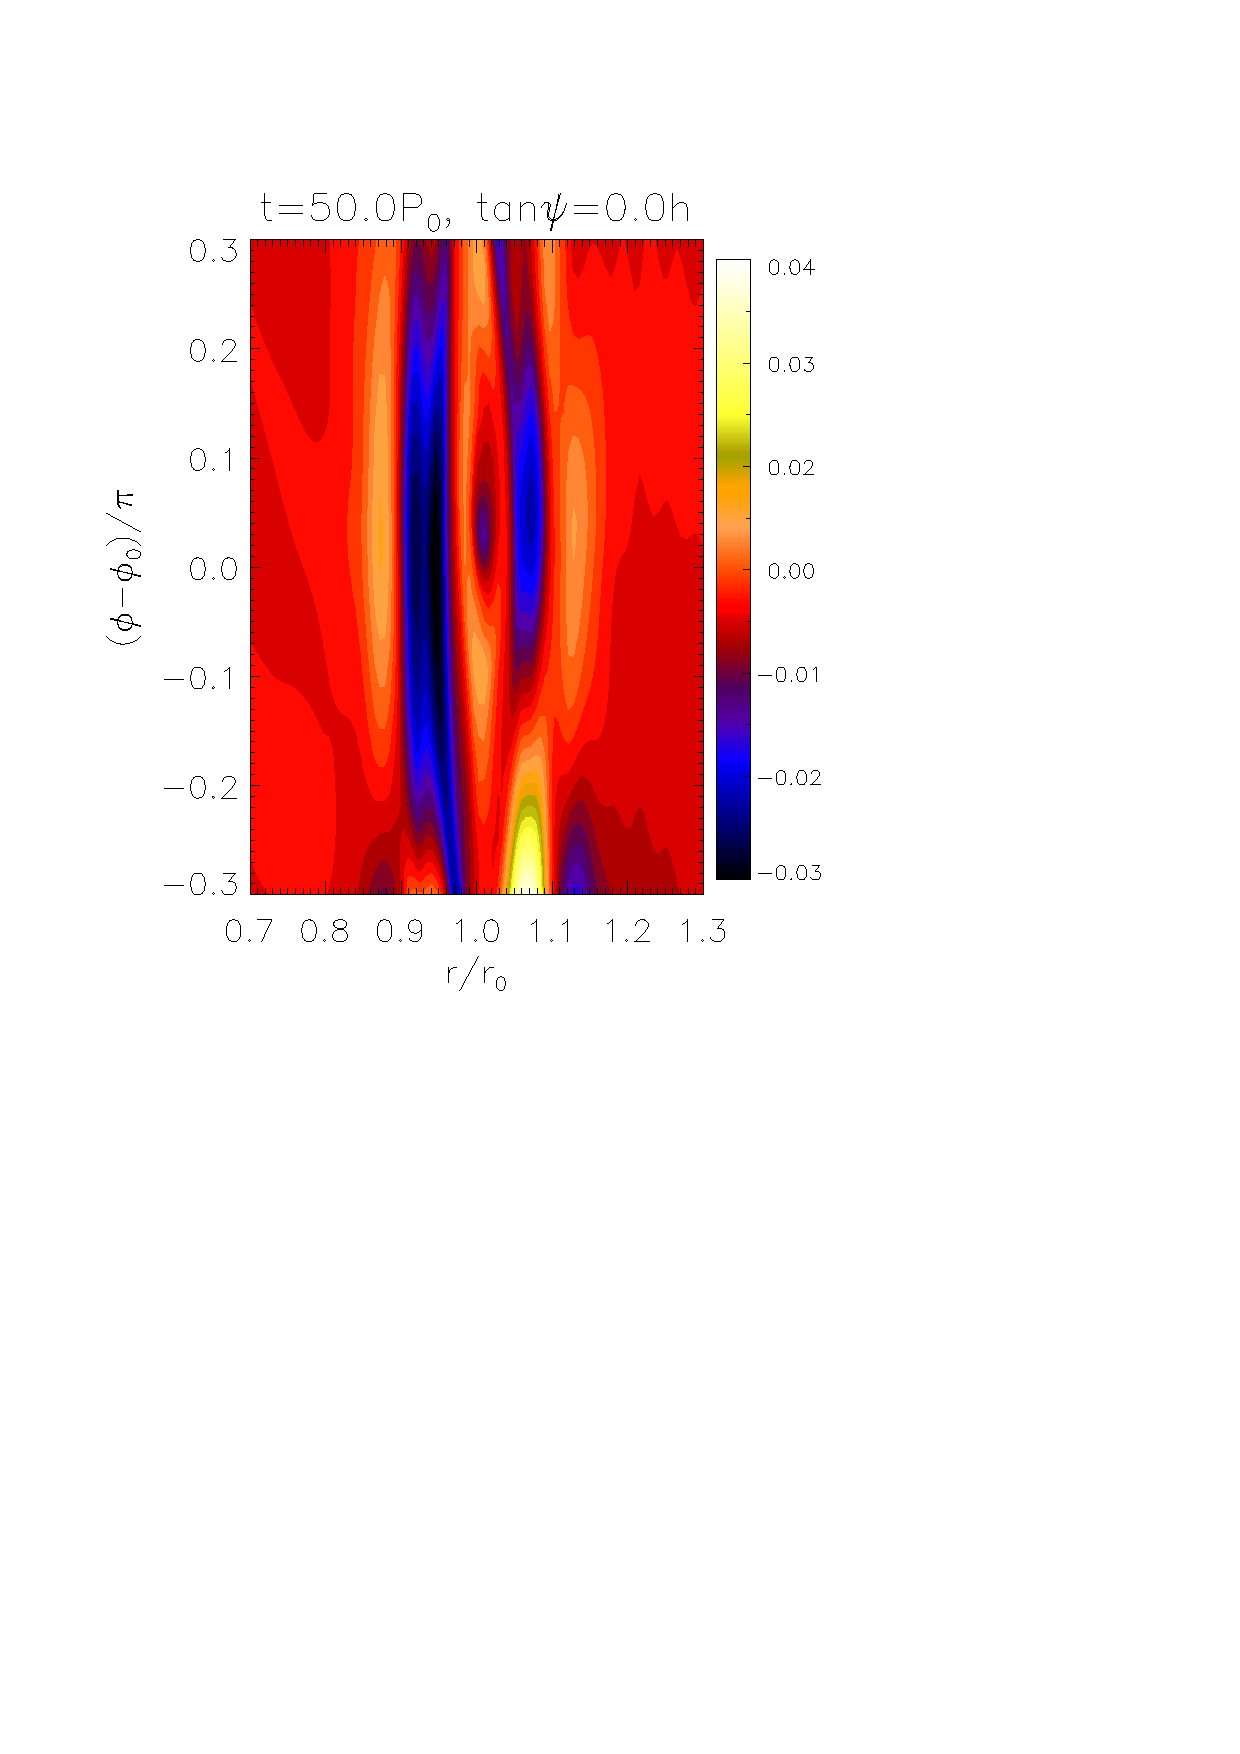
\includegraphics[scale=.27,clip=true,trim=2.3cm
     0.cm 0.cm
     0.99cm]{figures/bump1_vort014}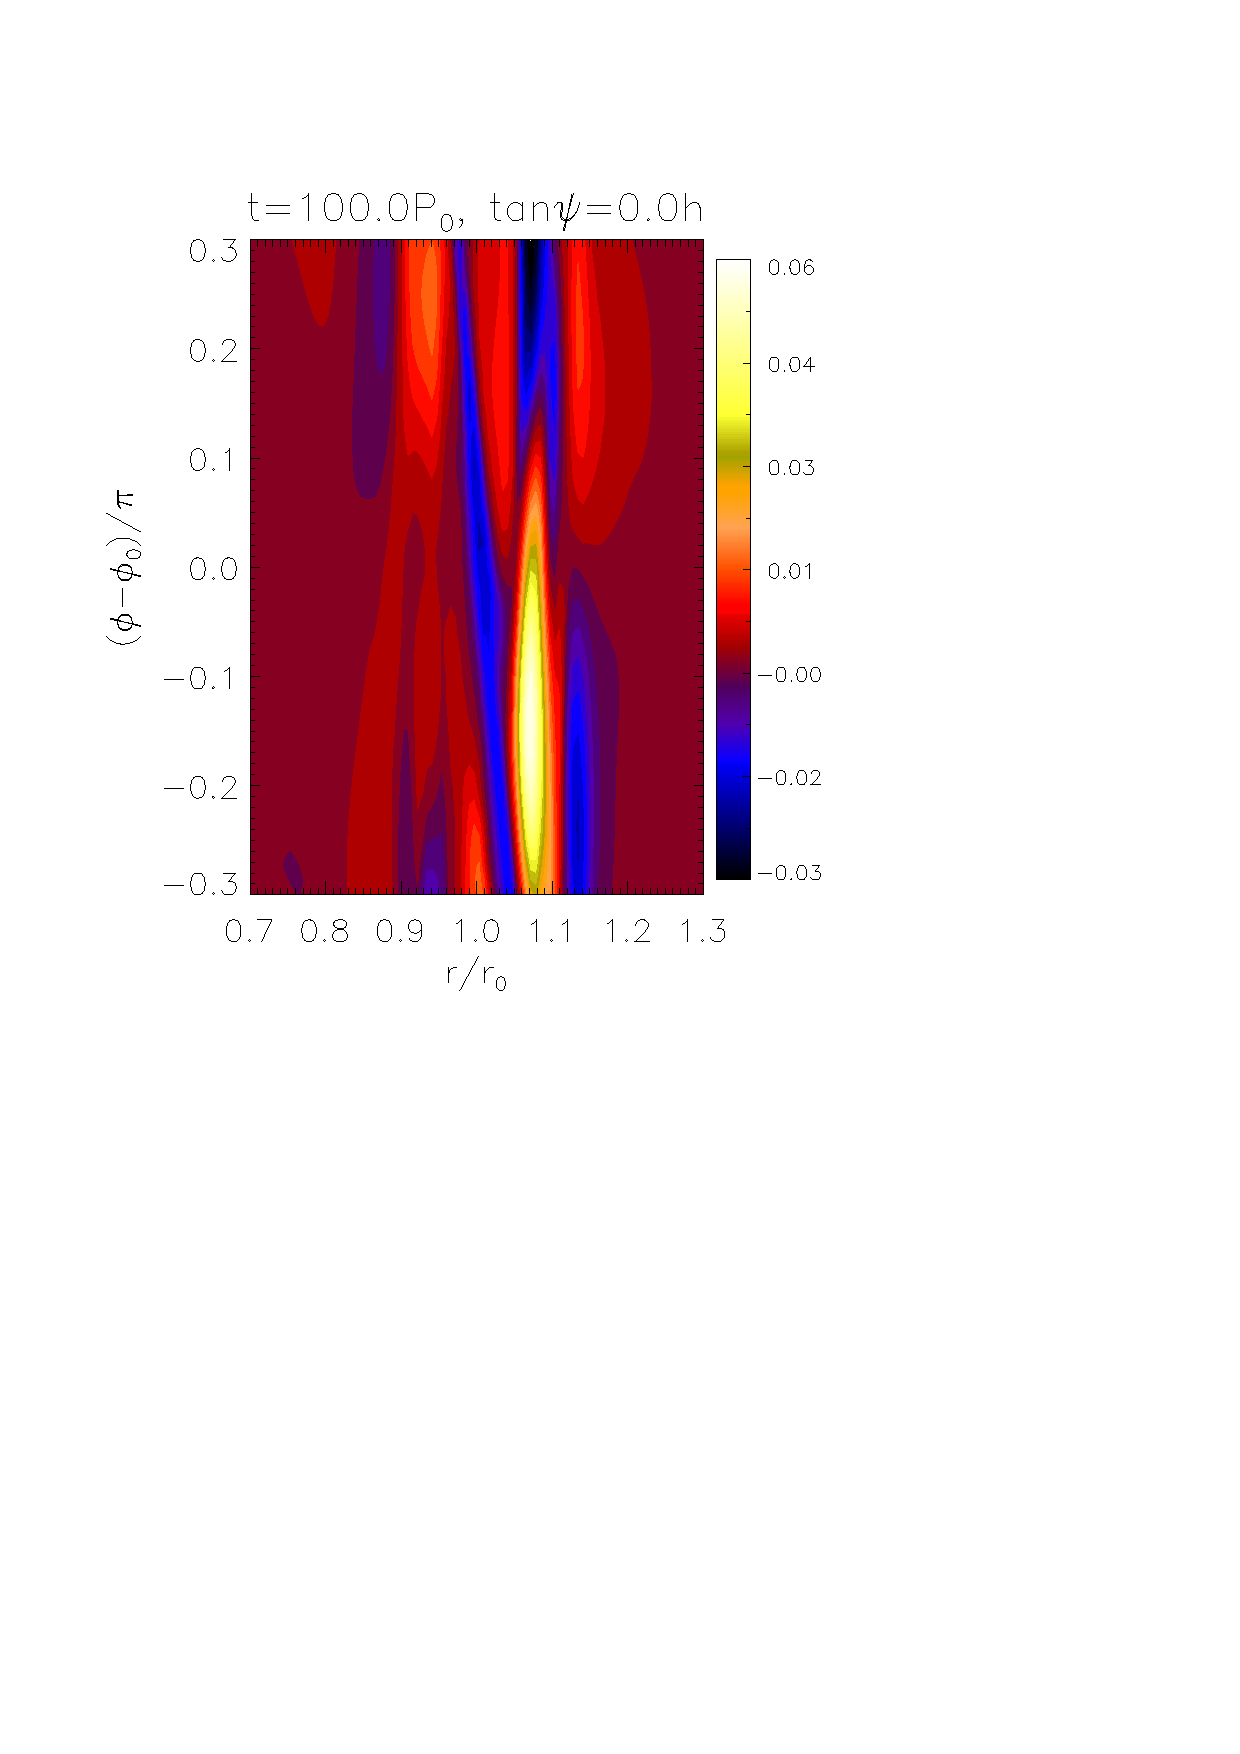
\includegraphics[scale=.27,clip=true,clip=true,trim=2.3cm
     0.cm 0.cm
     0.99cm]{figures/bump1_vort019}
   \caption{Evolution of the midplane Rossby number, $Ro(z=0)$, for case B0 with a reflective upper boundary (top) and case
     B1  with an unperturbed upper boundary (bottom). $\chi$ is the
     width-to-length aspect ratio of the dotted boxes. 
   \label{bump0_bump1_vort}}
 \end{figure}

\subsection{Appending a viscous upper layer}
Case V0 is the fiducial viscous run with vertical domain size $\tan{\psimax}=2h$, and
kinematic viscosity $\hat{\nu}\sim10^{-6}$ throughout the
computational domain. This case only differs from the inviscid case B0
in the magnitude of viscosity. Neither simulation employ the
layered viscosity profile described earlier. 

Comparing case V0 to case B0, Table \ref{artificial_bump} shows that
linear growth rates are unaffected by a viscosity of magnitude
$\hat{\nu}\lesssim10^{-6}$. Even in the non-linear regime, the 
disturbance amplitude $a_m$ is only slightly smaller with larger
viscosity, corresponding to a slightly weaker vortex. 

We now introduce a high-viscosity layer. Case V0e has a vertical
domain size $\tan{\psimax}=3h$, with $\hat{\nu}\sim 10^{-6}$ for
$\tan{\psi} < 2h$, and $\hat{\nu}\sim10^{-4}$ for $\tan{\psi}>2h$. In
other words, case V0e is the same as case V0, but with a viscous
atmosphere of thickness $h$ appended on top.  

The linear growth rate for case V0e is smaller than case V0, but only
by about $\sim 6\%$. 
%% Note that there could be a contribution to this decrease from the
%% evolution of the axisymmetric background, because the initial state is
%% not a prefect equilibrium. Low resolution
%% runs without initial seed perturbations yield an increase in 
%% the azimuthally-averaged vortensity field (relative to the initial
%% state) by $10\%$ and $1\%$ at the bump radius at $t=10P_0$ for case V0
%% and case V0e, respectively. 
Interestingly, the non-linear mode amplitude $a_m(100P_0)$ is
slightly larger with a viscous atmosphere and the final vortex is
stronger. 

Fig. \ref{vdamp0_vdamp1_3h} and Fig. \ref{vdamp0_vdamp1_3h_vort}
compares the non-linear evolution of case V0 and case V0e. In both
cases the final configuration is a single vortex. In case V0
the vortex weakens (elongates), with both $\max(\Delta\rho)$ and
$\max(|Ro|)$ decreasing by a factor of $\sim2$ by the end of the
simulation. However, the vortex in case V0e maintains
$\max(\Delta\rho)\sim 0.4$. The Rossby number evolves very differently
in case V0e, and $\min(Ro)$ is always more negative than case
V0. Furthermore, the vortex in fact shrinks with time. 

%(though early on it is smaller than case V0)
%figures indicate den pert more global in v0e

 \begin{figure}
   \centering
   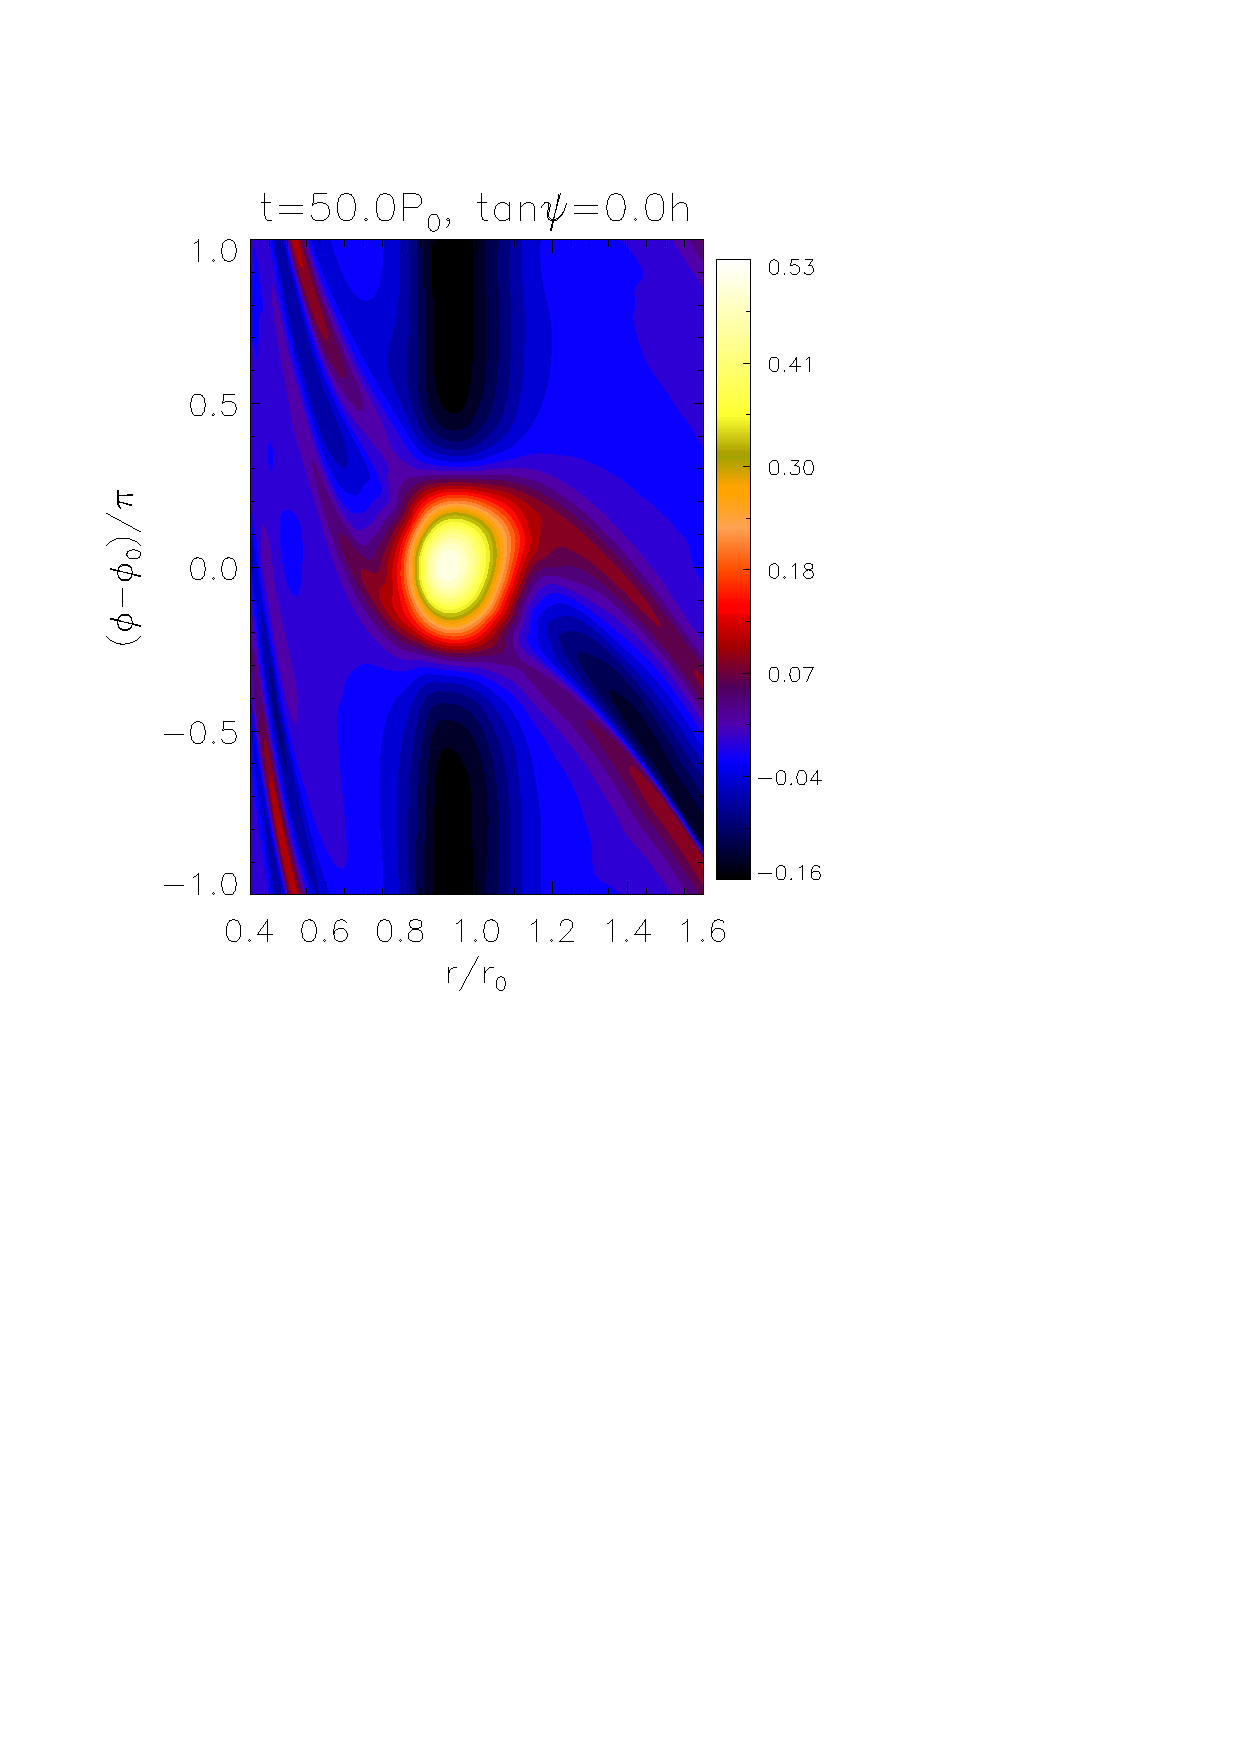
\includegraphics[scale=.27,clip=true,trim=0cm 1.84cm 0cm
     0cm]{figures/vdamp0_pdisk014}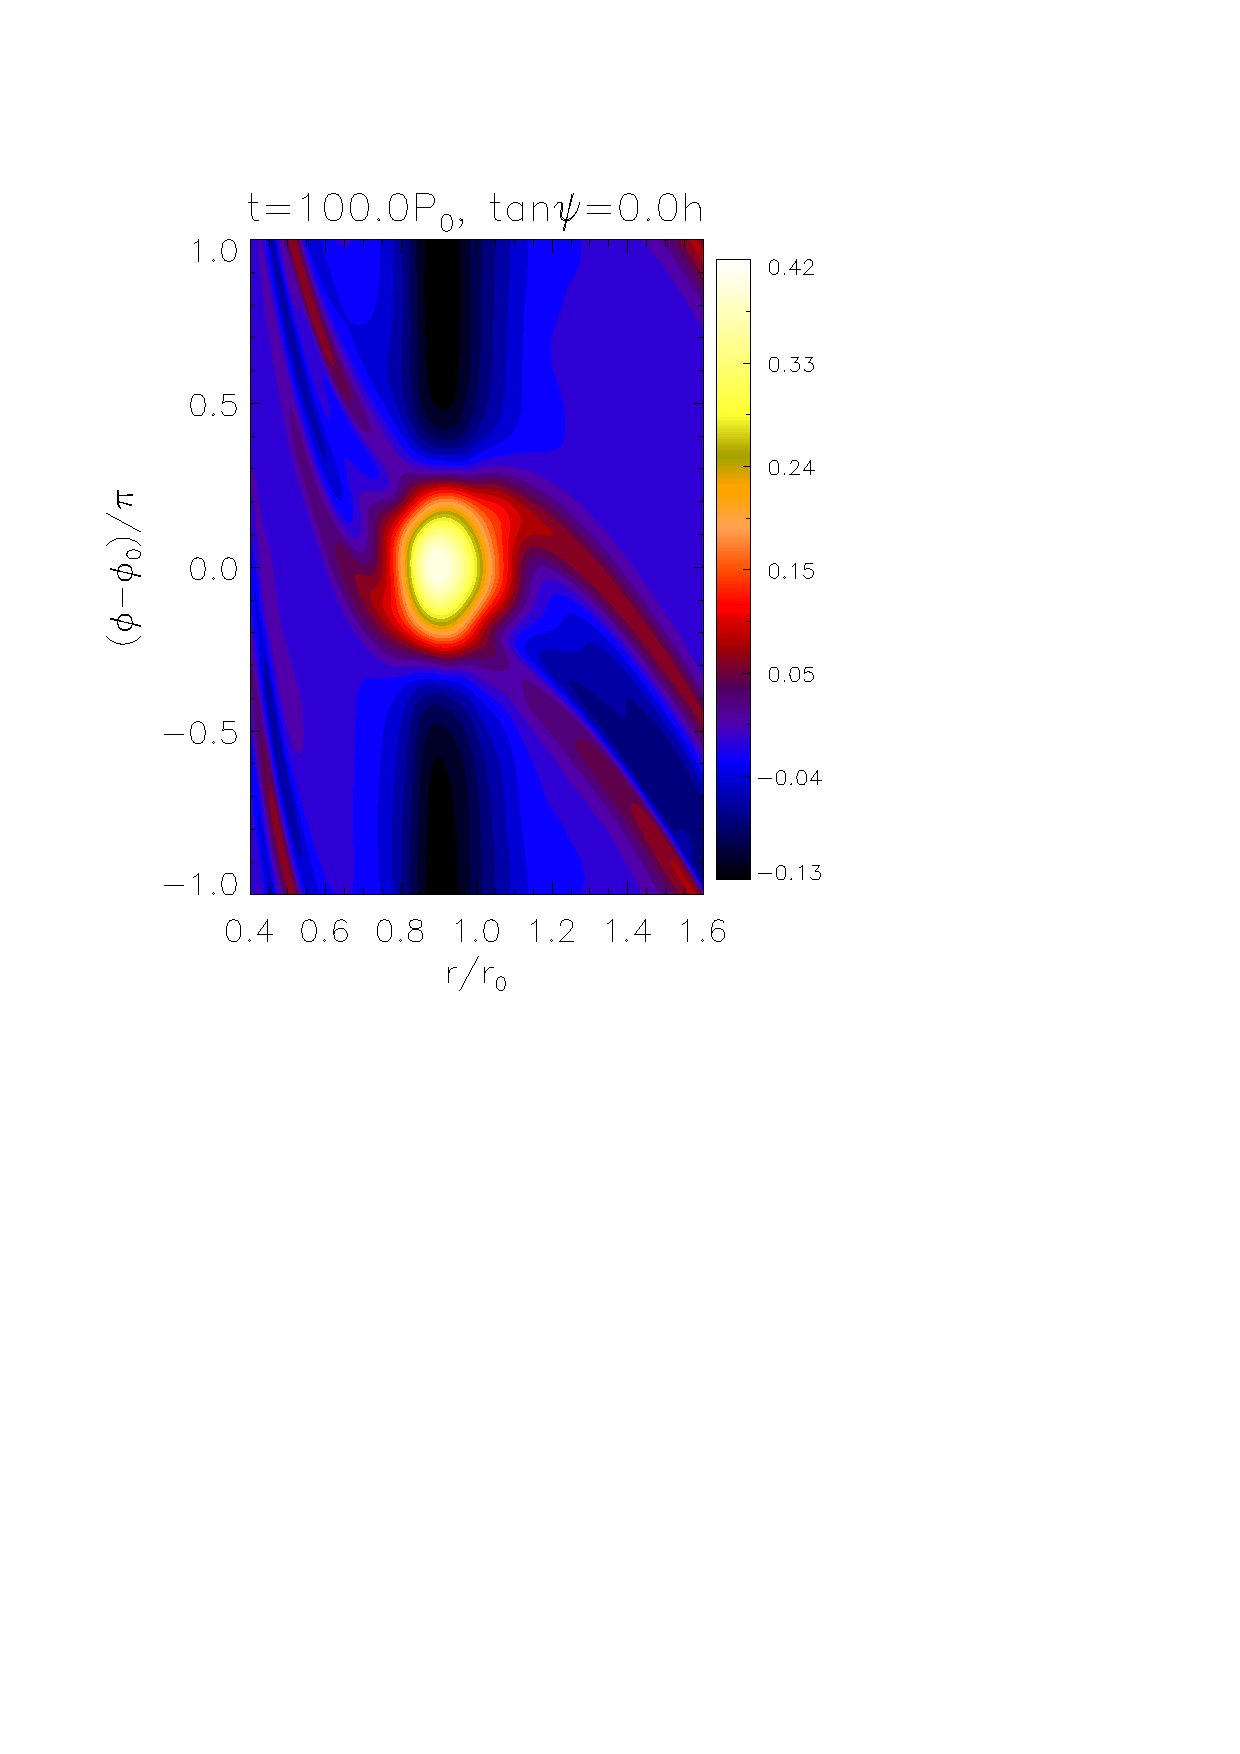
\includegraphics[scale=.27,clip=true,trim=2.3cm
     1.84cm 0cm
     0cm]{figures/vdamp0_pdisk019}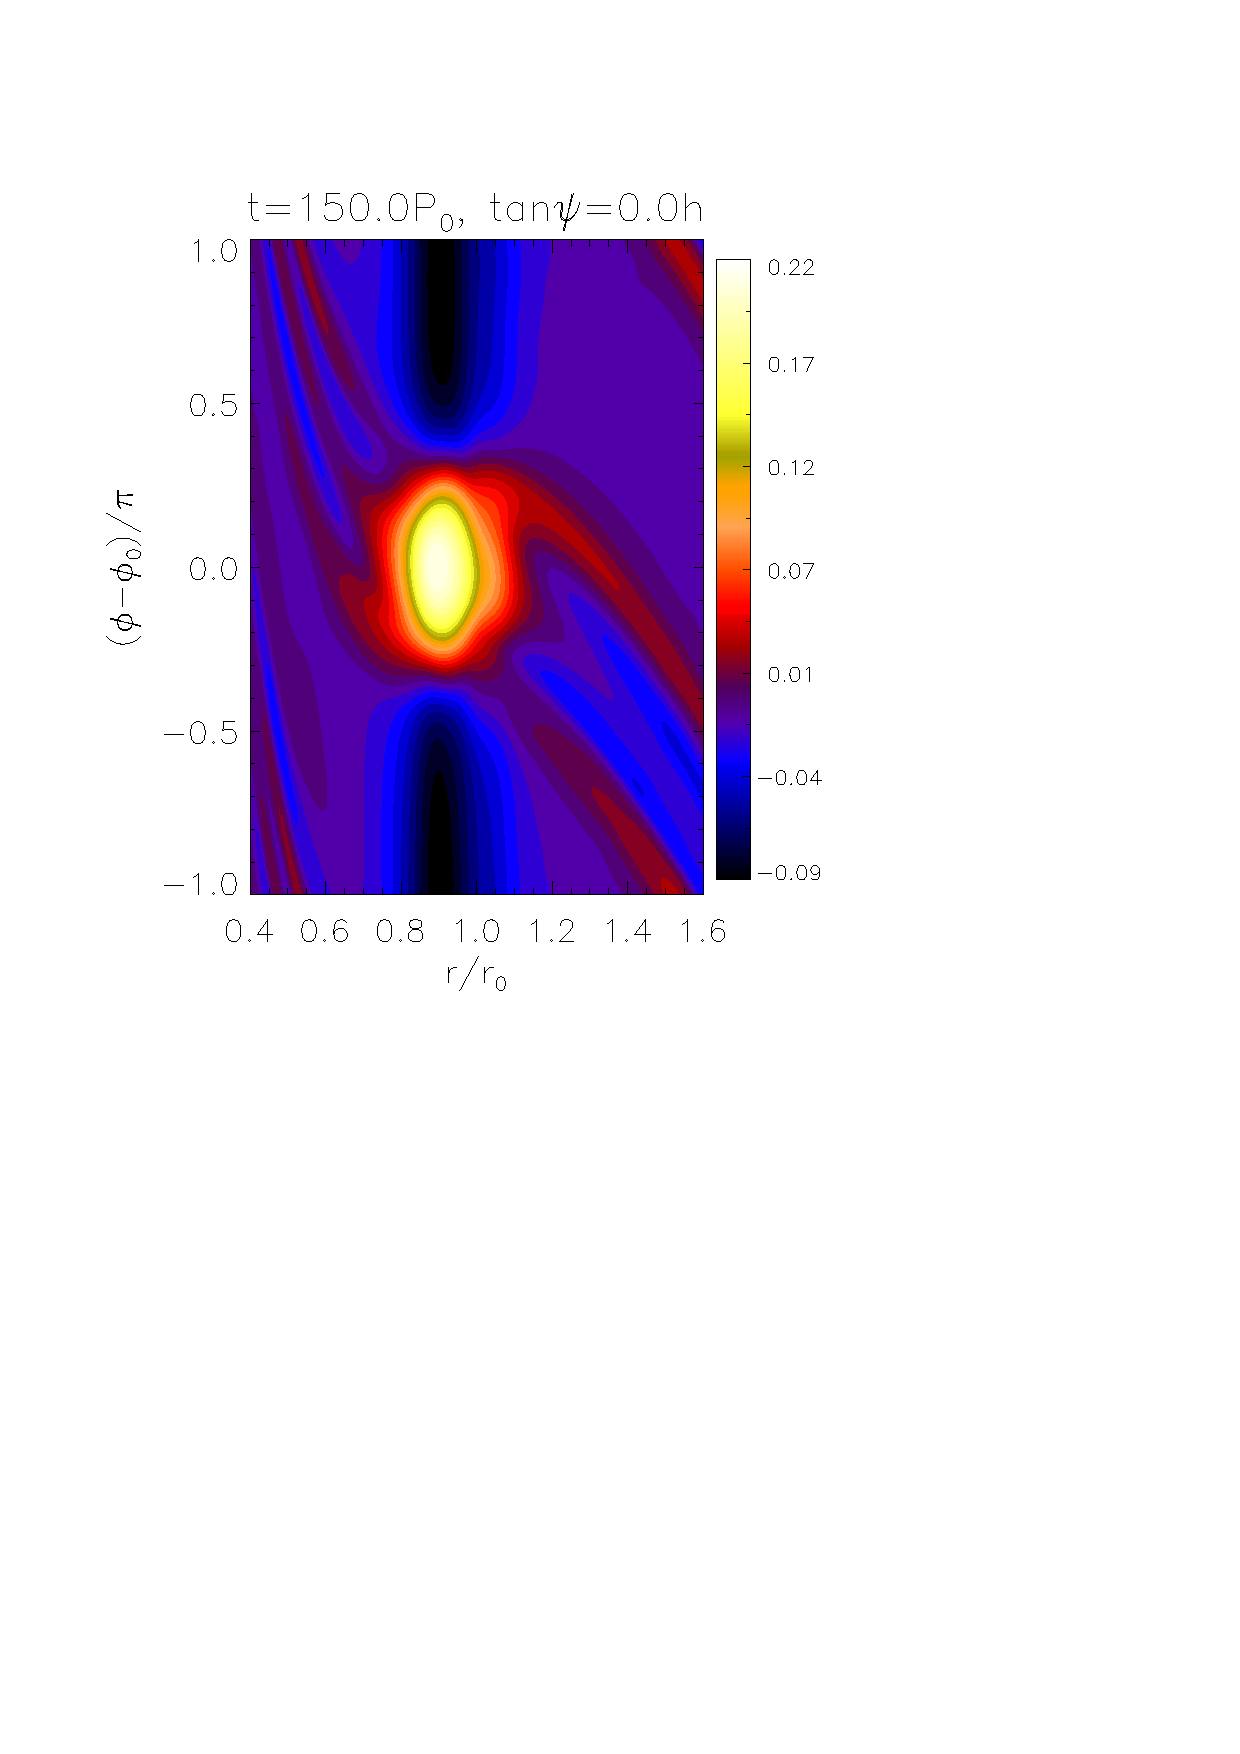
\includegraphics[scale=.27,clip=true,clip=true,trim=2.3cm
     1.84cm 0cm
     0cm]{figures/vdamp0_pdisk024}\\
   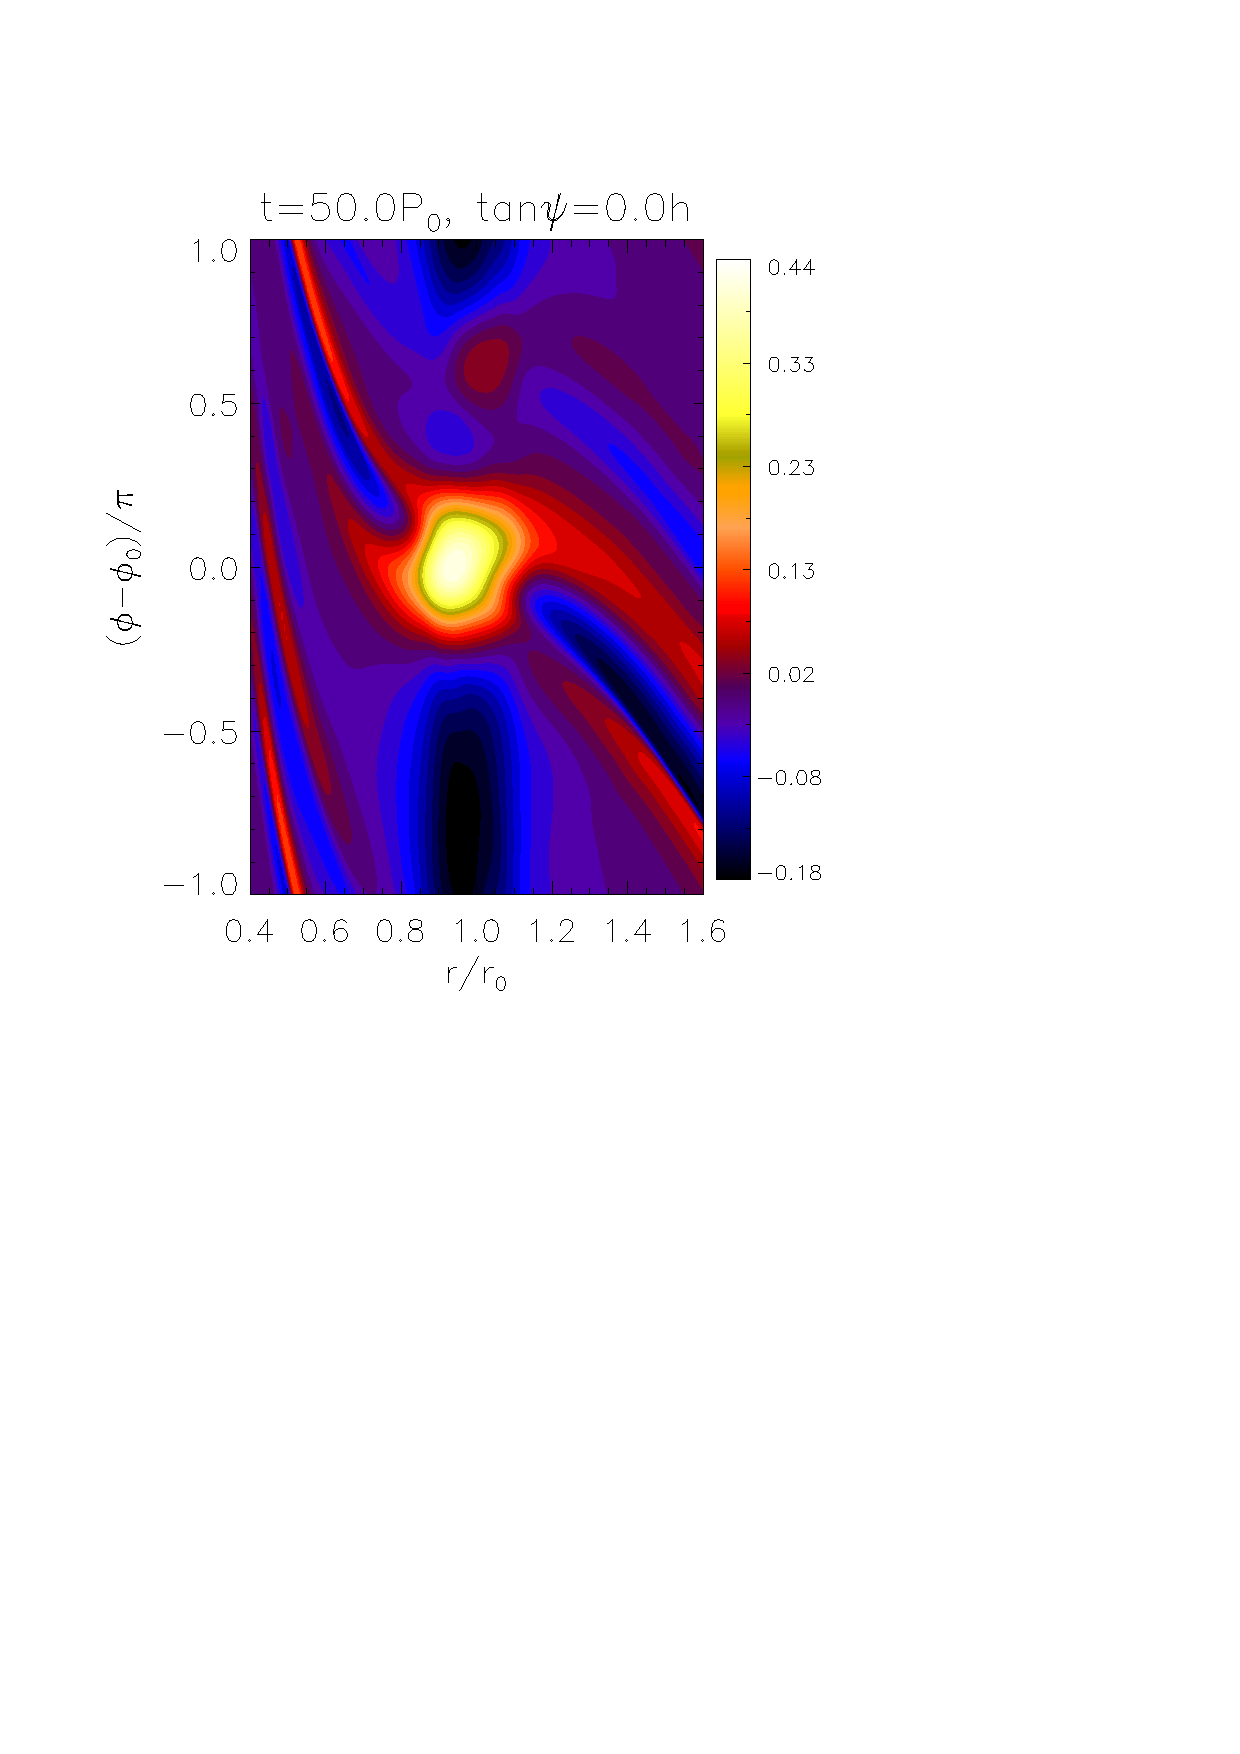
\includegraphics[scale=.27,clip=true,trim=0cm 0.cm 0.0cm
     0.99cm]{figures/vdamp1_3h_pdisk014}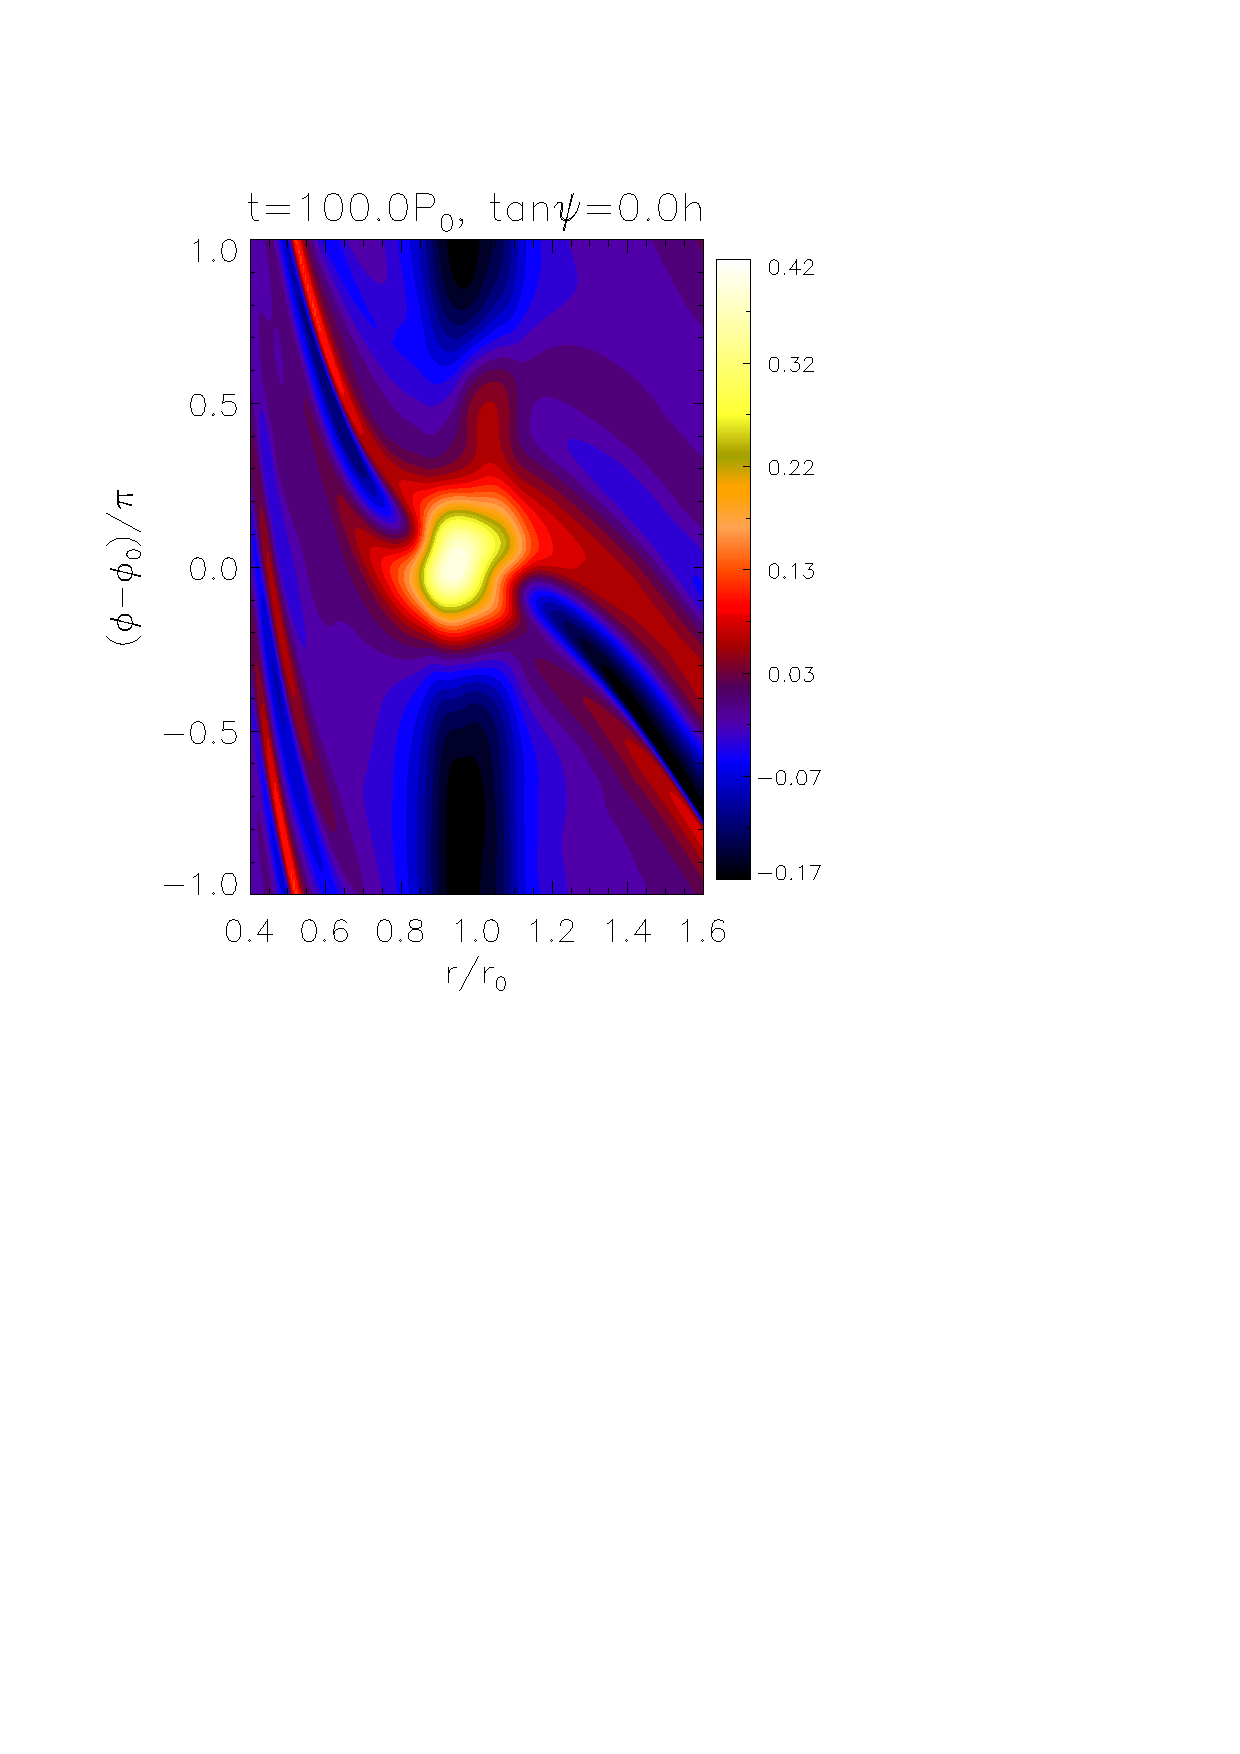
\includegraphics[scale=.27,clip=true,trim=2.3cm
     0.cm 0.cm
     0.99cm]{figures/vdamp1_3h_pdisk019}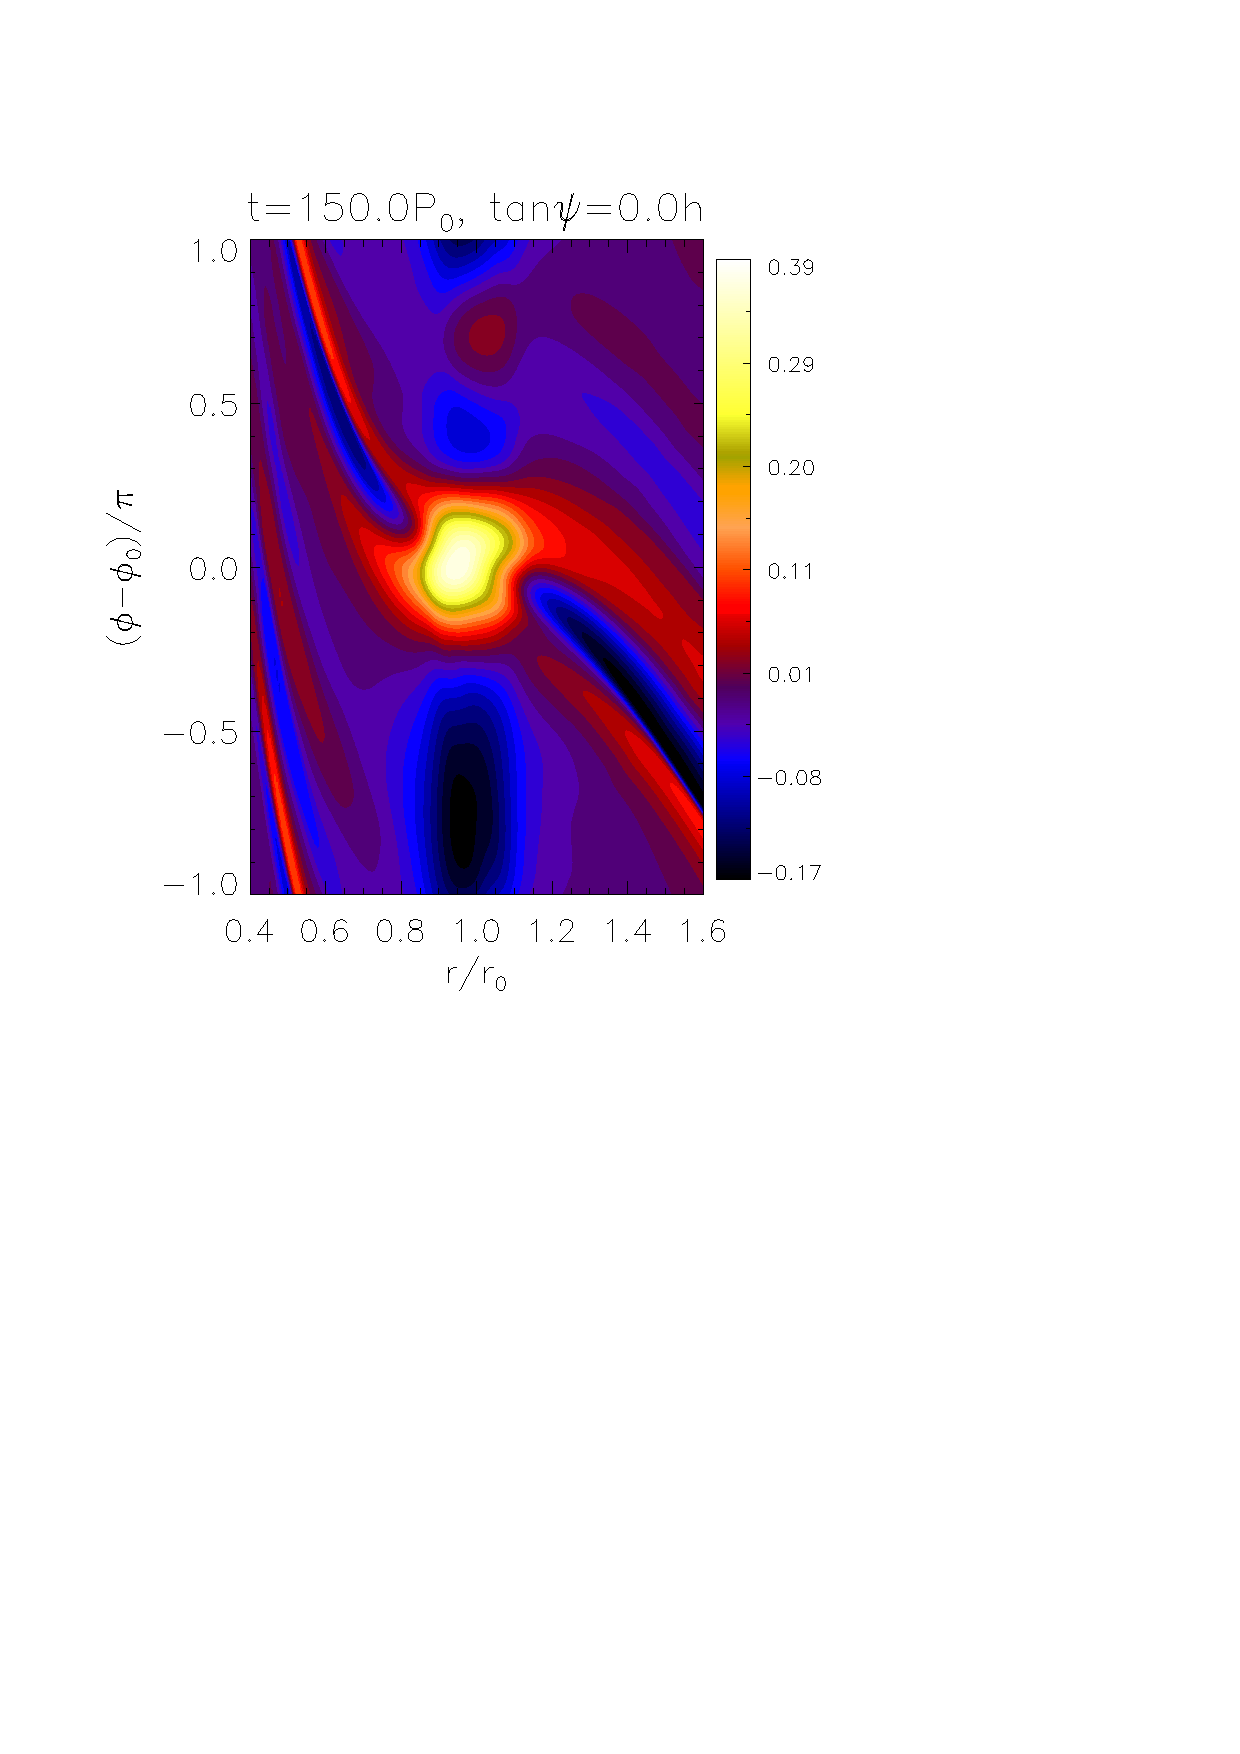
\includegraphics[scale=.27,clip=true,clip=true,trim=2.3cm
     0.cm 0.cm
     0.99cm]{figures/vdamp1_3h_pdisk024}  
   \caption{Evolution of the midplane non-axisymmetric density field,
     $\Delta\rho(z=0)$, for the fiducial viscous case V0 (top), and case  
     V0e (bottom). Both cases have a dimensionless kinematic viscosity
     $\hat{\nu}\sim 10^{-6}$ in the bulk of the disc, but case V1e has
     an atmosphere of thickness $H$ within which $\hat{\nu}\sim 10^{-4}$ (see
     Table \ref{artificial_bump}). 
     %% $\phi_0$ is the
     %% azimuth of $\mathrm{max}(|\Delta\rho(z=0)|)$. 
   \label{vdamp0_vdamp1_3h}}
 \end{figure}


\begin{figure}
   \centering
   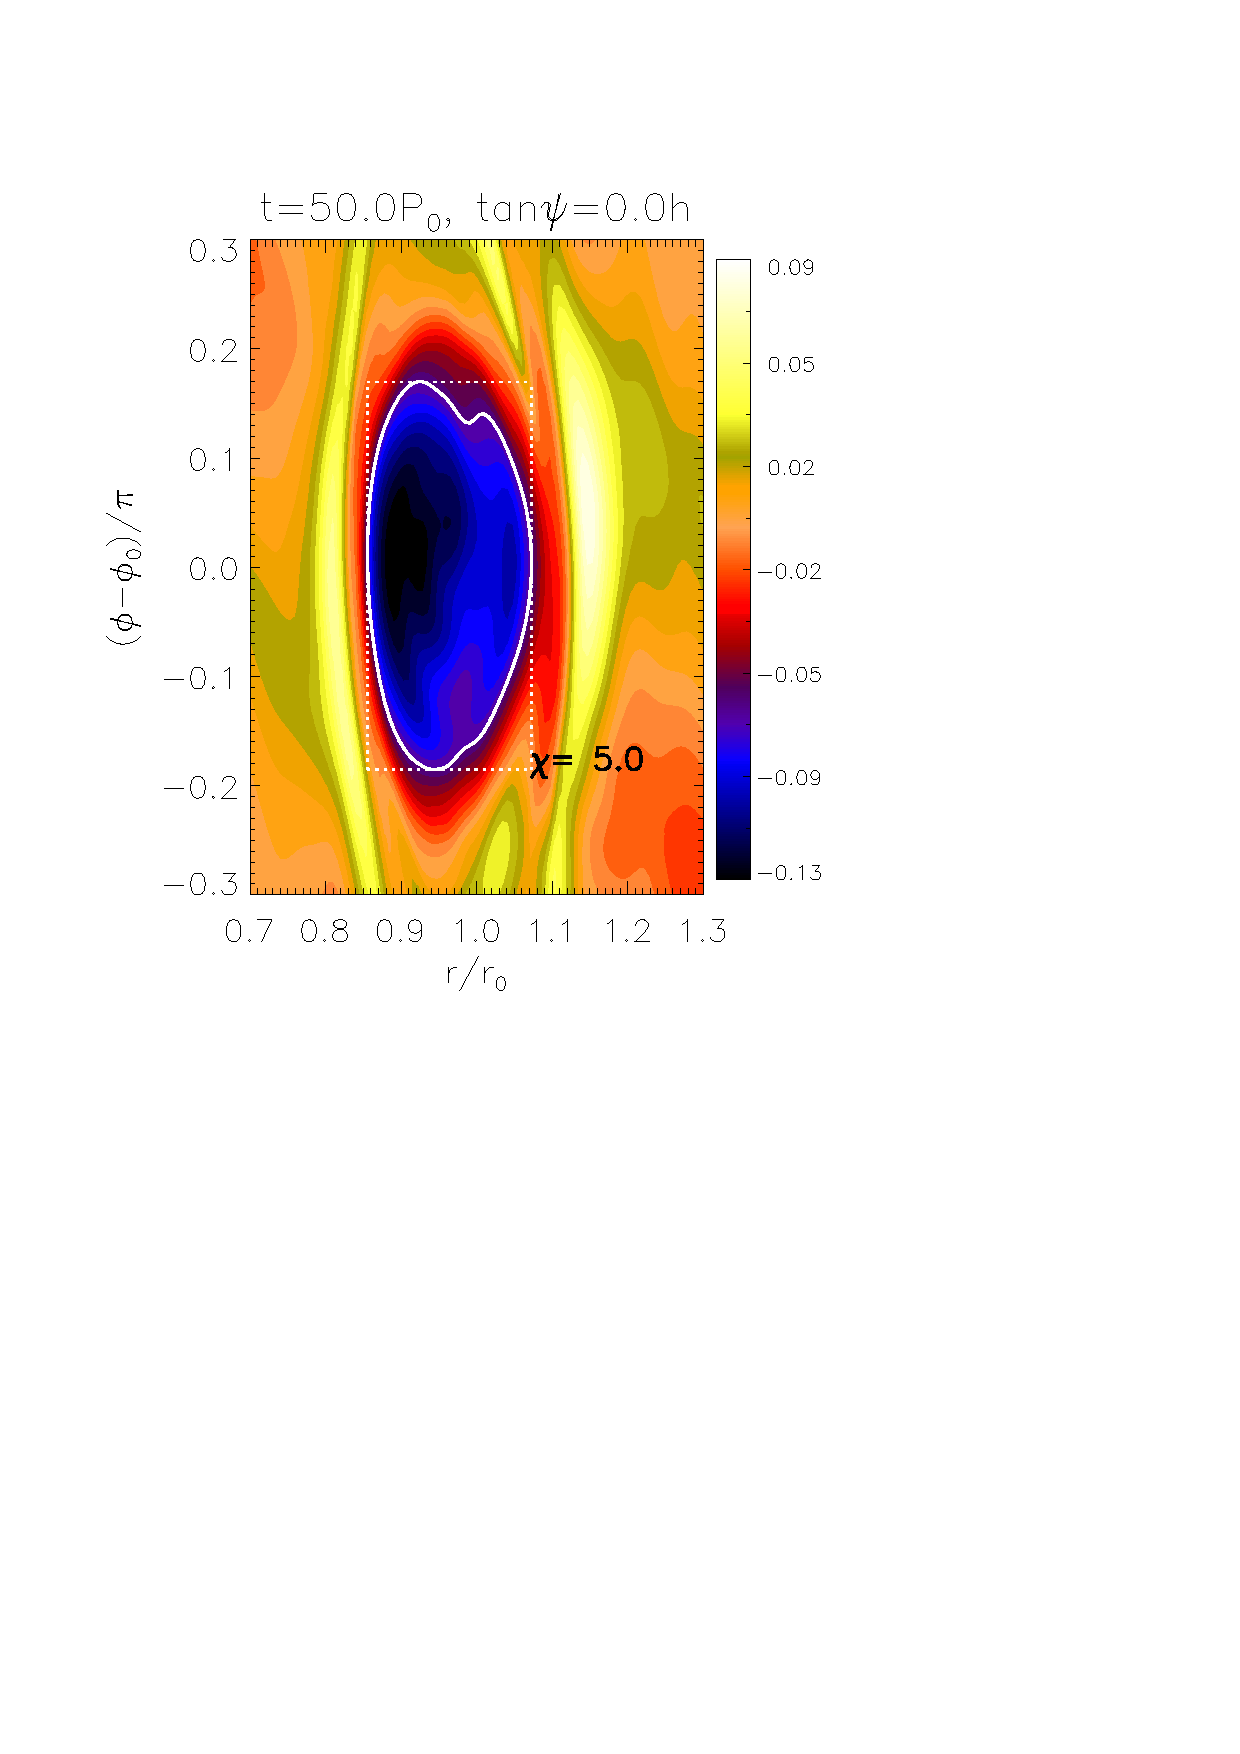
\includegraphics[scale=.27,clip=true,trim=0cm 1.84cm 0cm
     0cm]{figures/vdamp0_vort014}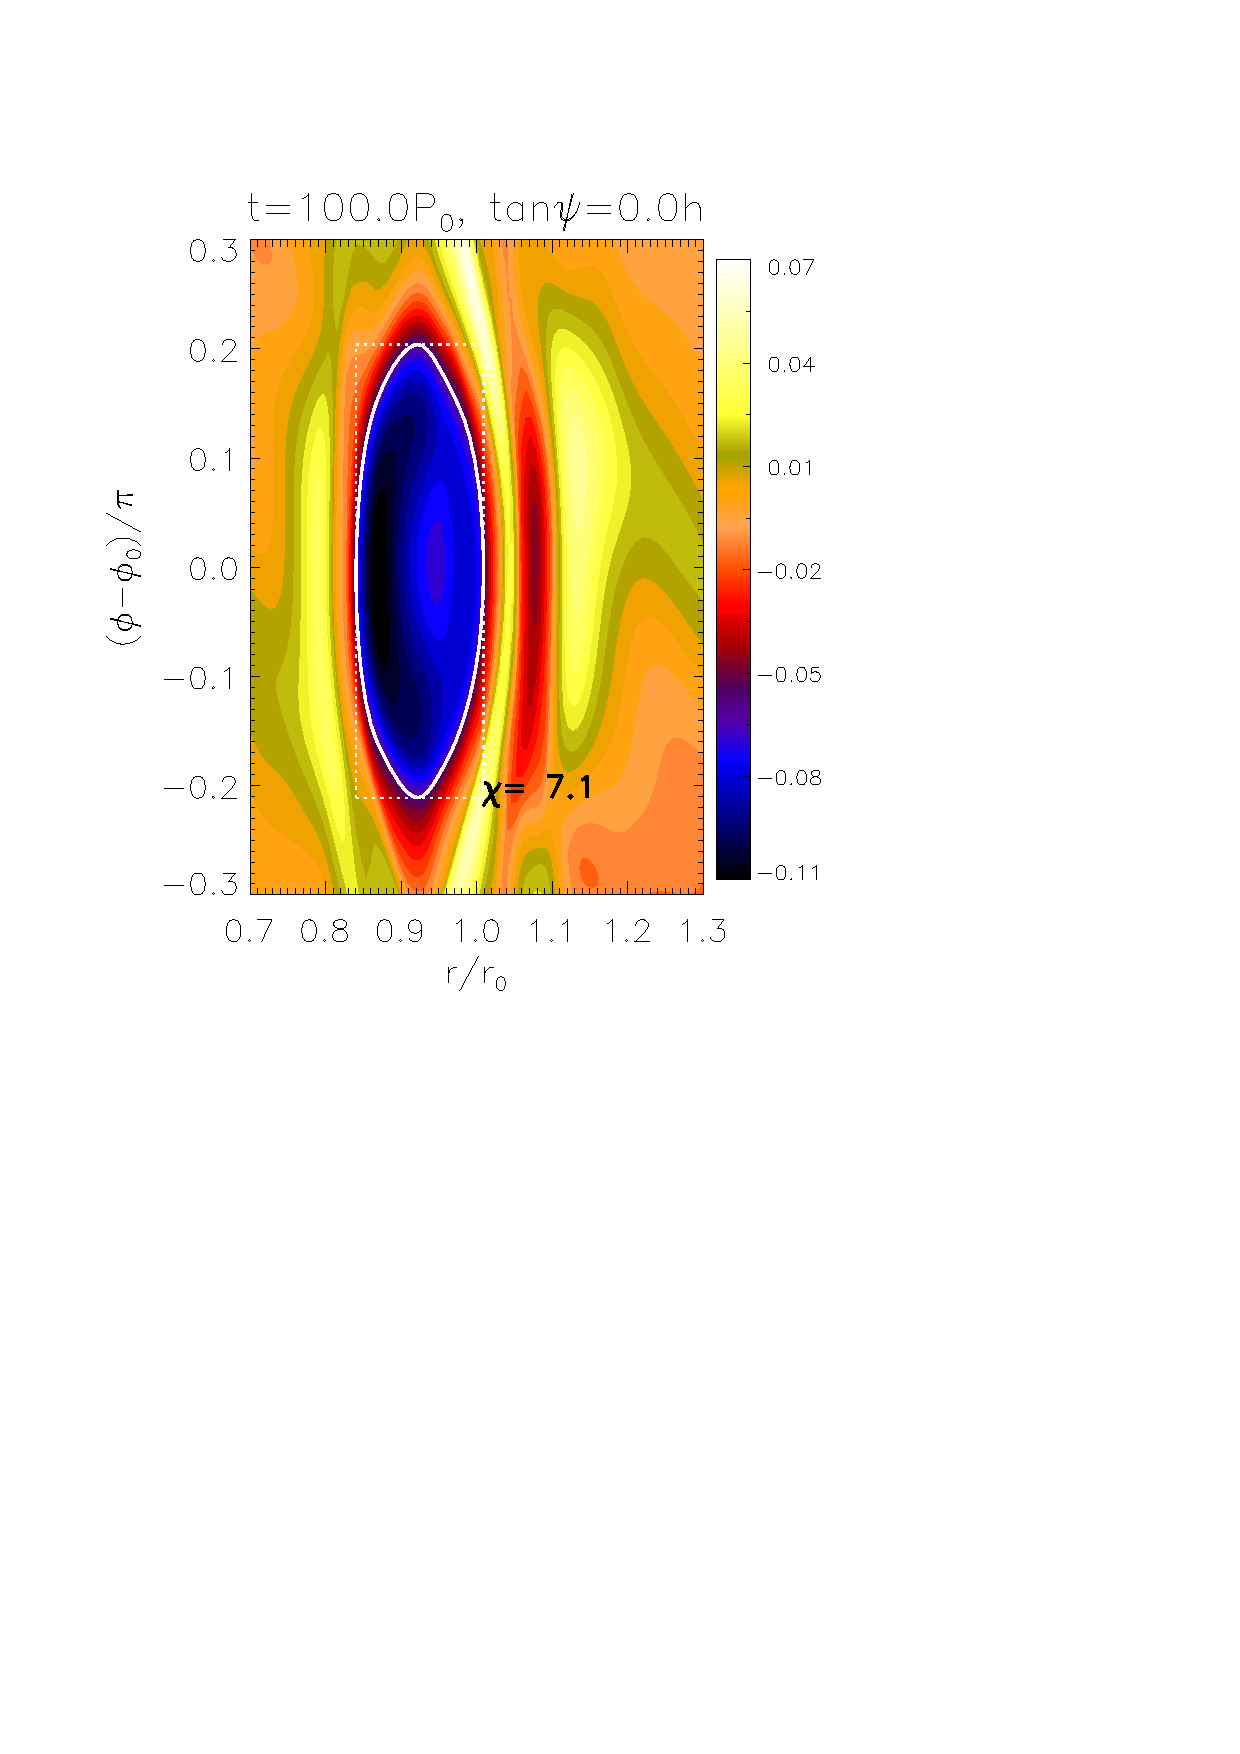
\includegraphics[scale=.27,clip=true,trim=2.3cm
     1.84cm 0cm
     0cm]{figures/vdamp0_vort019}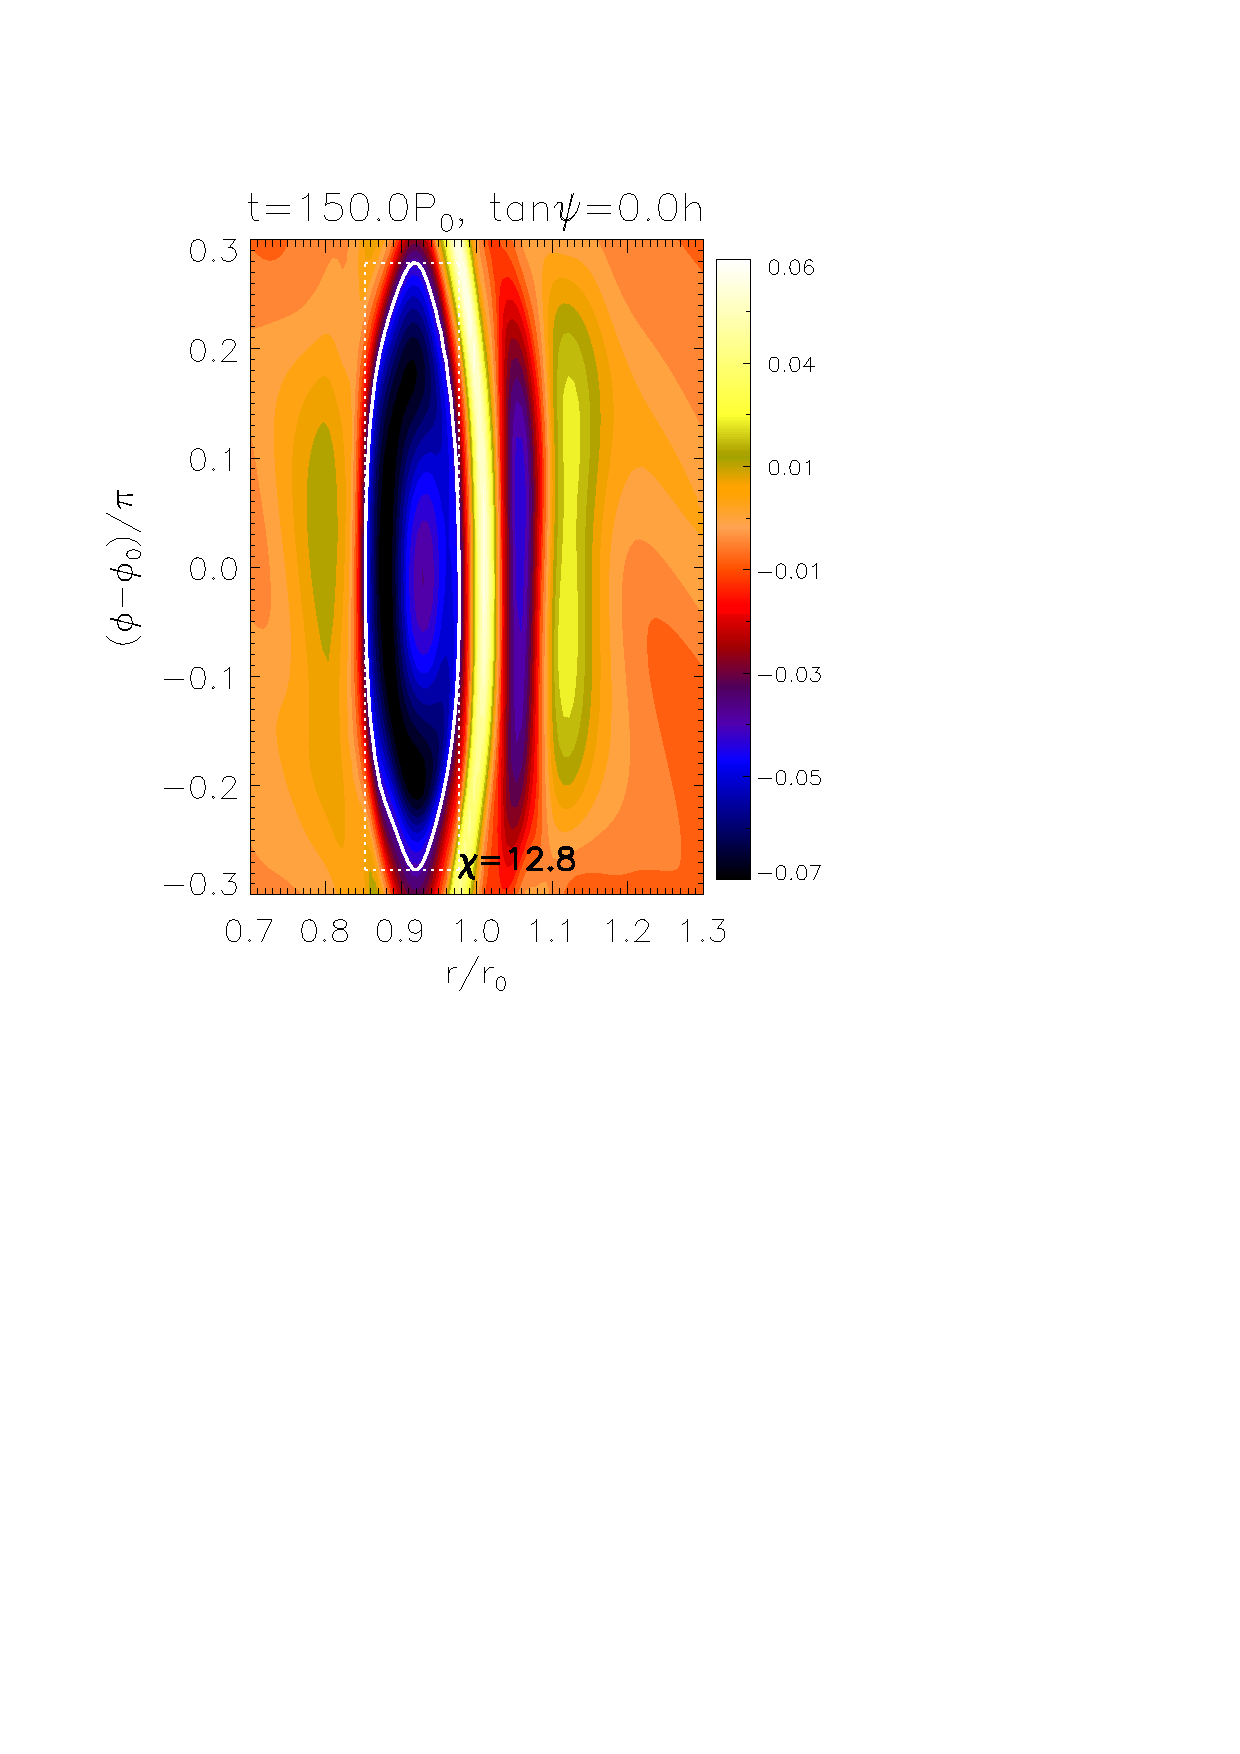
\includegraphics[scale=.27,clip=true,clip=true,trim=2.3cm
     1.84cm 0cm
     0cm]{figures/vdamp0_vort024}\\
   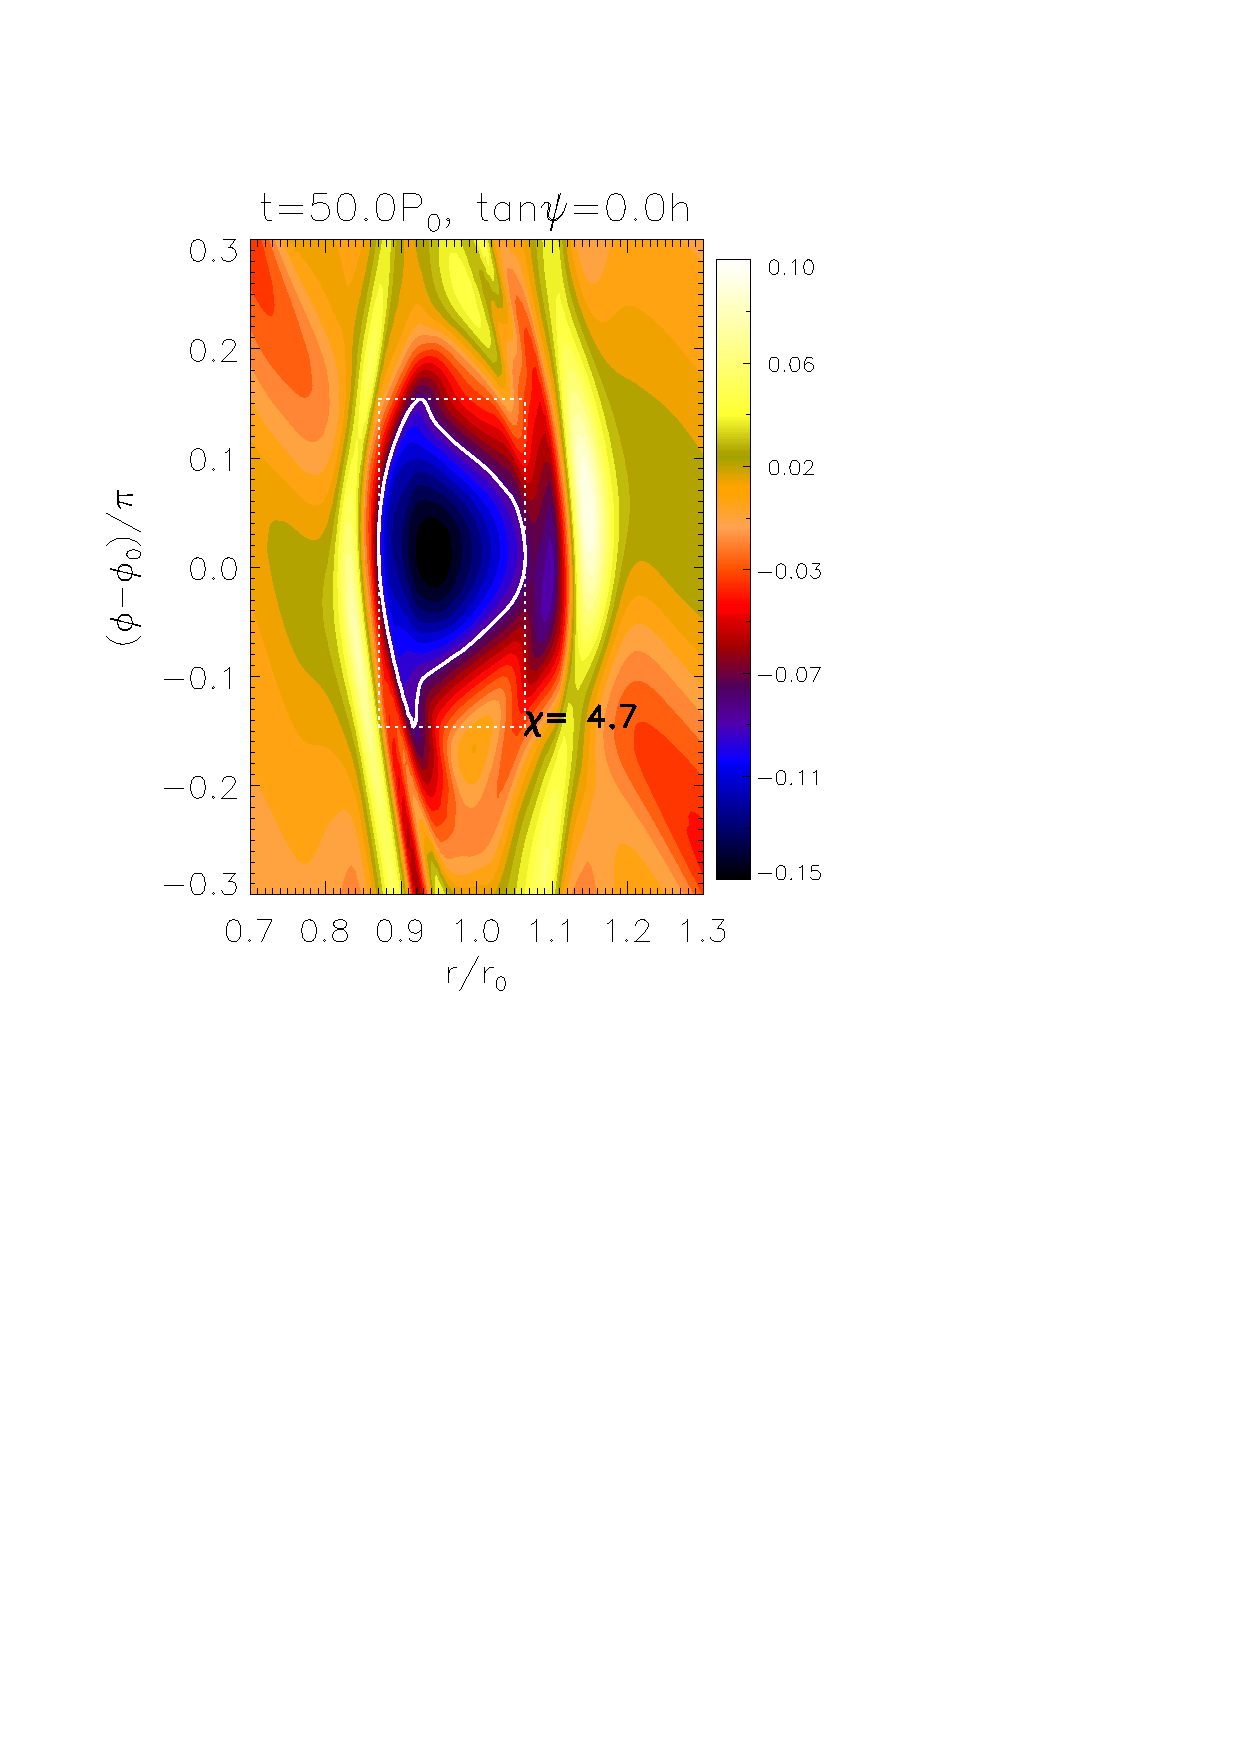
\includegraphics[scale=.27,clip=true,trim=0cm 0.cm 0.0cm
     0.99cm]{figures/vdamp1_3h_vort014}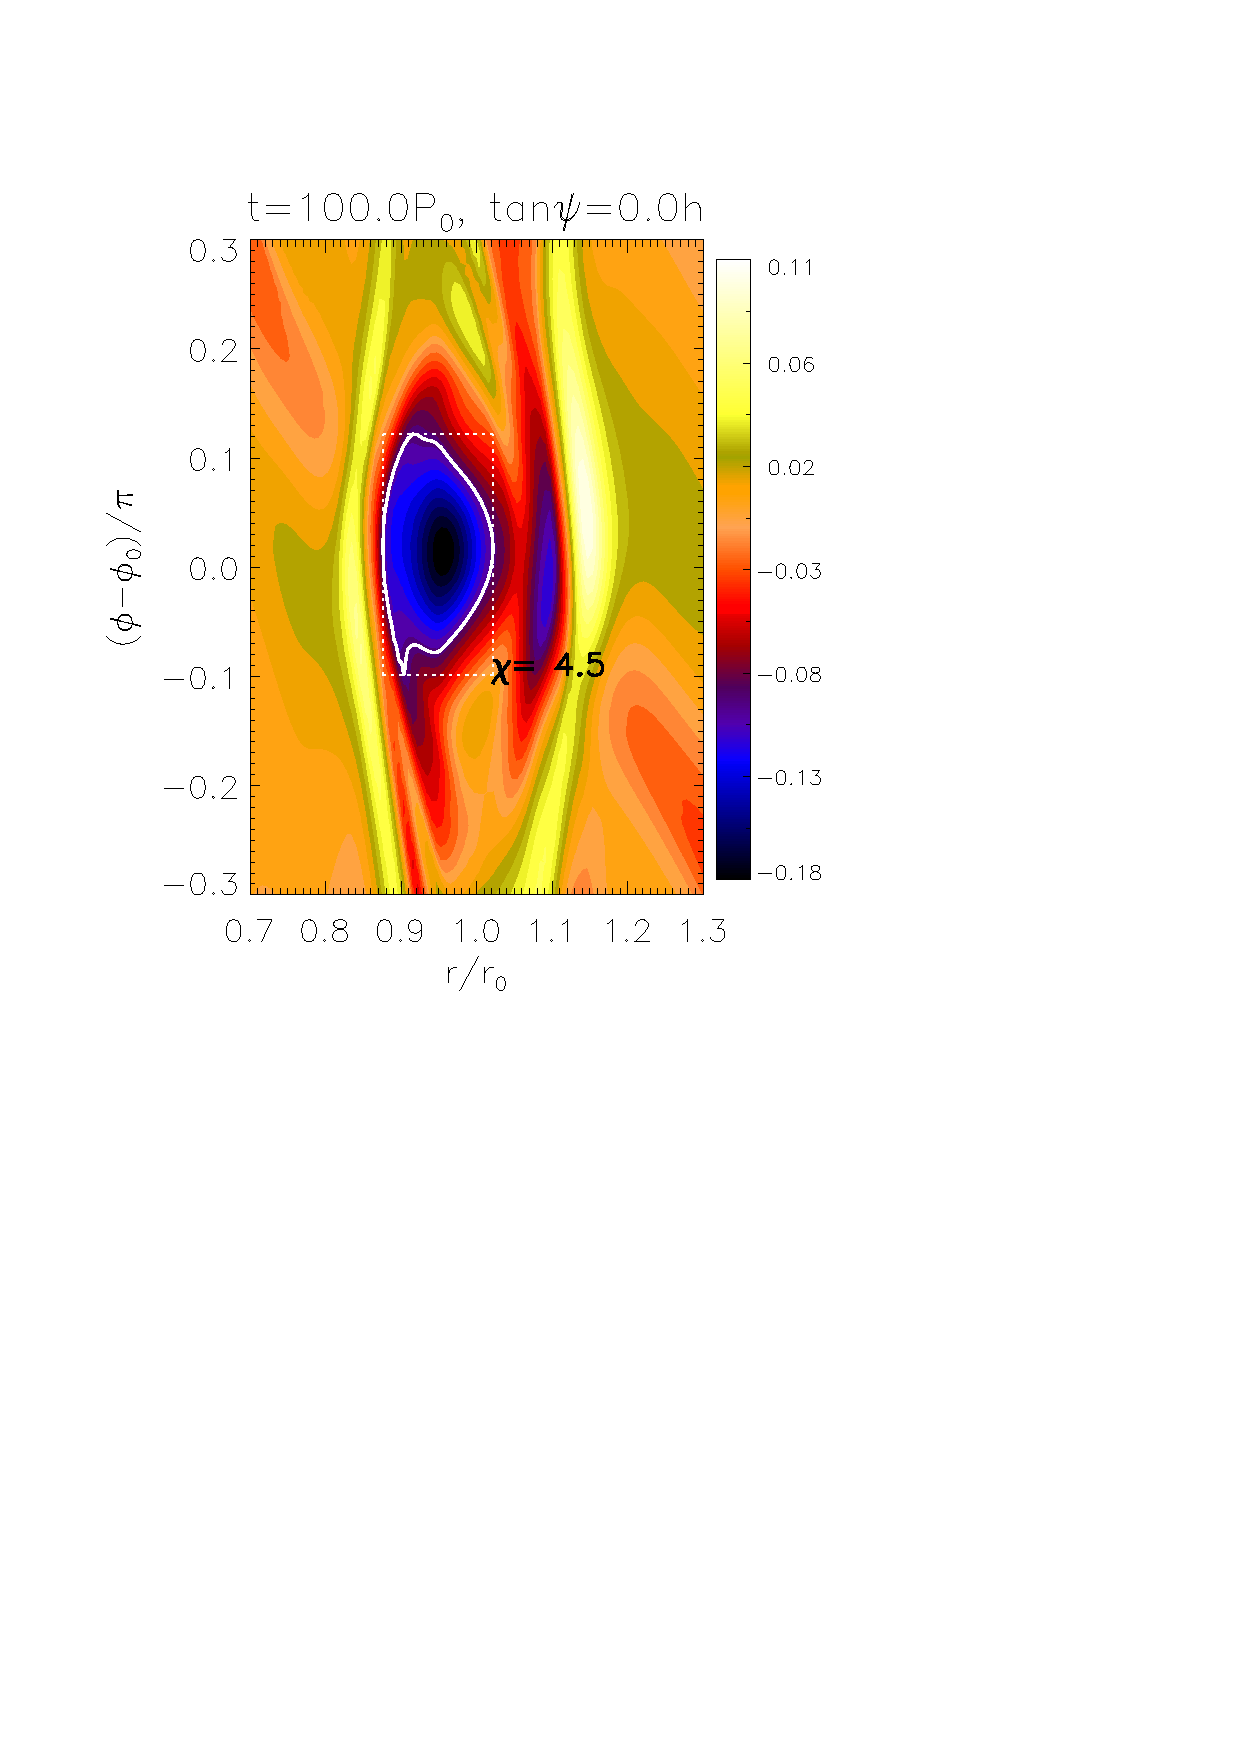
\includegraphics[scale=.27,clip=true,trim=2.3cm
     0.cm 0.cm
     0.99cm]{figures/vdamp1_3h_vort019}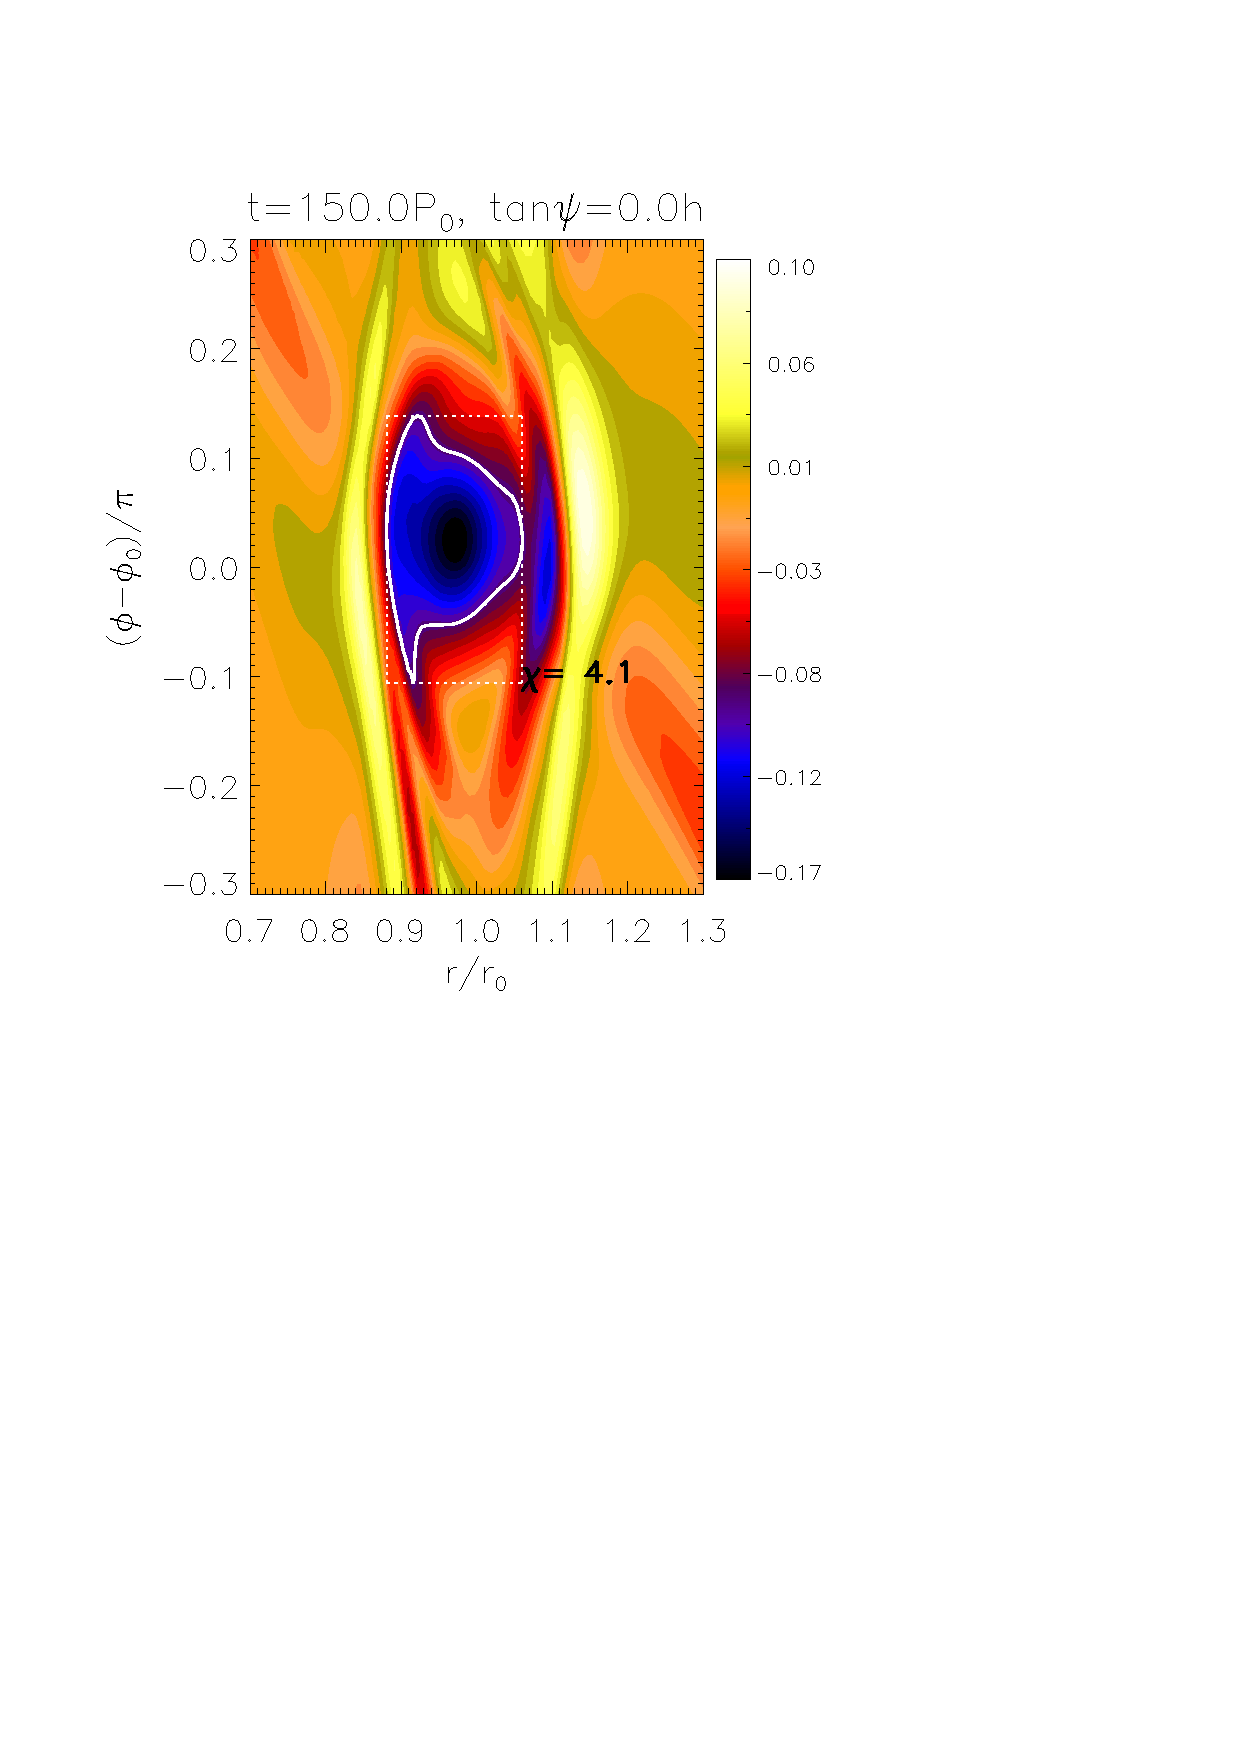
\includegraphics[scale=.27,clip=true,clip=true,trim=2.3cm
     0.cm 0.cm
     0.99cm]{figures/vdamp1_3h_vort024}
   \caption{Evolution of the midplane Rossby number, $Ro(z=0)$, for
     case V0 (top) and case V0e (bottom).
   \label{vdamp0_vdamp1_3h_vort}}
 \end{figure}

\subsection{Inserting viscous layers}
%The above result indicates that viscosity, when chosen to be
%(approximately) consistent with a steady-state disc containing a, 
%favours the formation of stronger vortices (more
%negative $Ro$) in the non-linear regime . We confirm this with further
%experiments below.  

Cases V1, V2 and V3 all employ the standard domain size
$\tan{\psimax}=2h$. Cases V1 and V2 use the two-layer viscosity
profile. The viscosity is $\hat{\nu}\sim 10^{-6}$ for
$\tan\psi < 1.5h$ in case V1, and for $\tan\psi < h$ in case
V2. Beyond these transitions, the viscosity is
$\hat{\nu}\sim10^{-4}$. Thus, case V1 (V2) has $25\%$ ($50\%$) of its
vertical domain with high-viscosity. Finally, we extend the
high-viscosity layer to occupy the entire vertical domain in case
V3, so it has no viscosity transition with respect to $\psi$. 

Table \ref{artificial_bump} shows that increasing the viscous layer thickness does not
change the dominant azimuthal wavenumber in the linear phase, but does appreciably decrease the 
linear growth rate (by $\sim 46\%$ from case V1 to V3). However, the growth time-scales are still
$O(P_0)$.  It remains fast compared to the viscous time-scale. So
viscosity does not significantly affect the linear phase.  

Fig. \ref{vdamp2} compares the non-axisymmetric density field at
$t=100P_0$ for cases V1, V2 and V3 described above. 
The dominant azimuthal wavenumber in the non-linear regime has increased in going from case
V1 to V3. Overall, $\Delta\rho$ becomes less concentrated near $r=r_0$, but $|\Delta\rho|$
decreases with increasing viscosity. It appears that, as the viscous layer is thickened,  
the system resists the non-linear process of vortex merging to produce a single vortex. 

Fig. \ref{vdamp2_vort} compares the Rossby number associated with the
over-densities identified above. This figure shows
that increasing the extent of the viscous layer leads to smaller 
vortices with more negative $Ro$, as observed in the previous experiment. The vortex aspect-ratio 
decreases.   


\begin{figure}
   \centering
   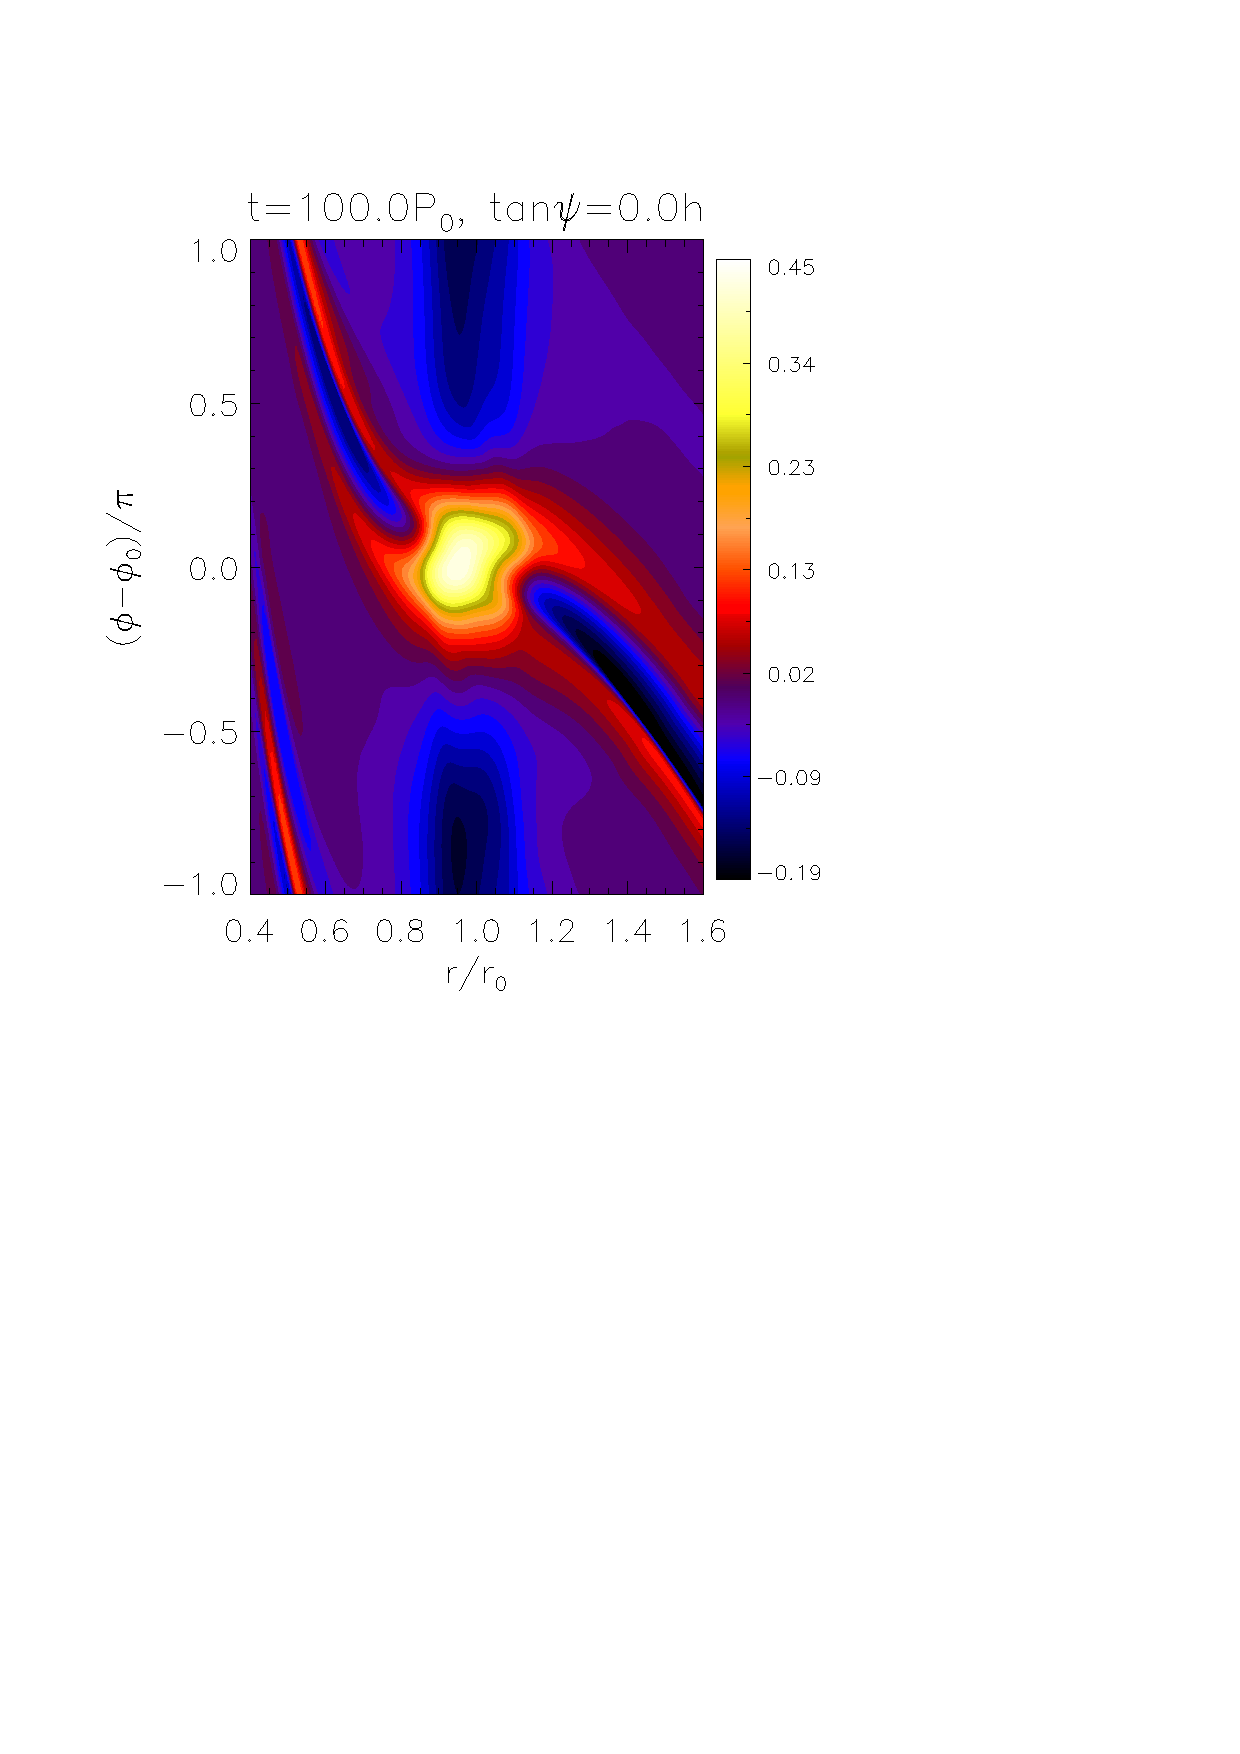
\includegraphics[scale=.27,clip=true,trim=0cm 0cm 0cm
     0cm]{figures/vdamp2_pdisk019}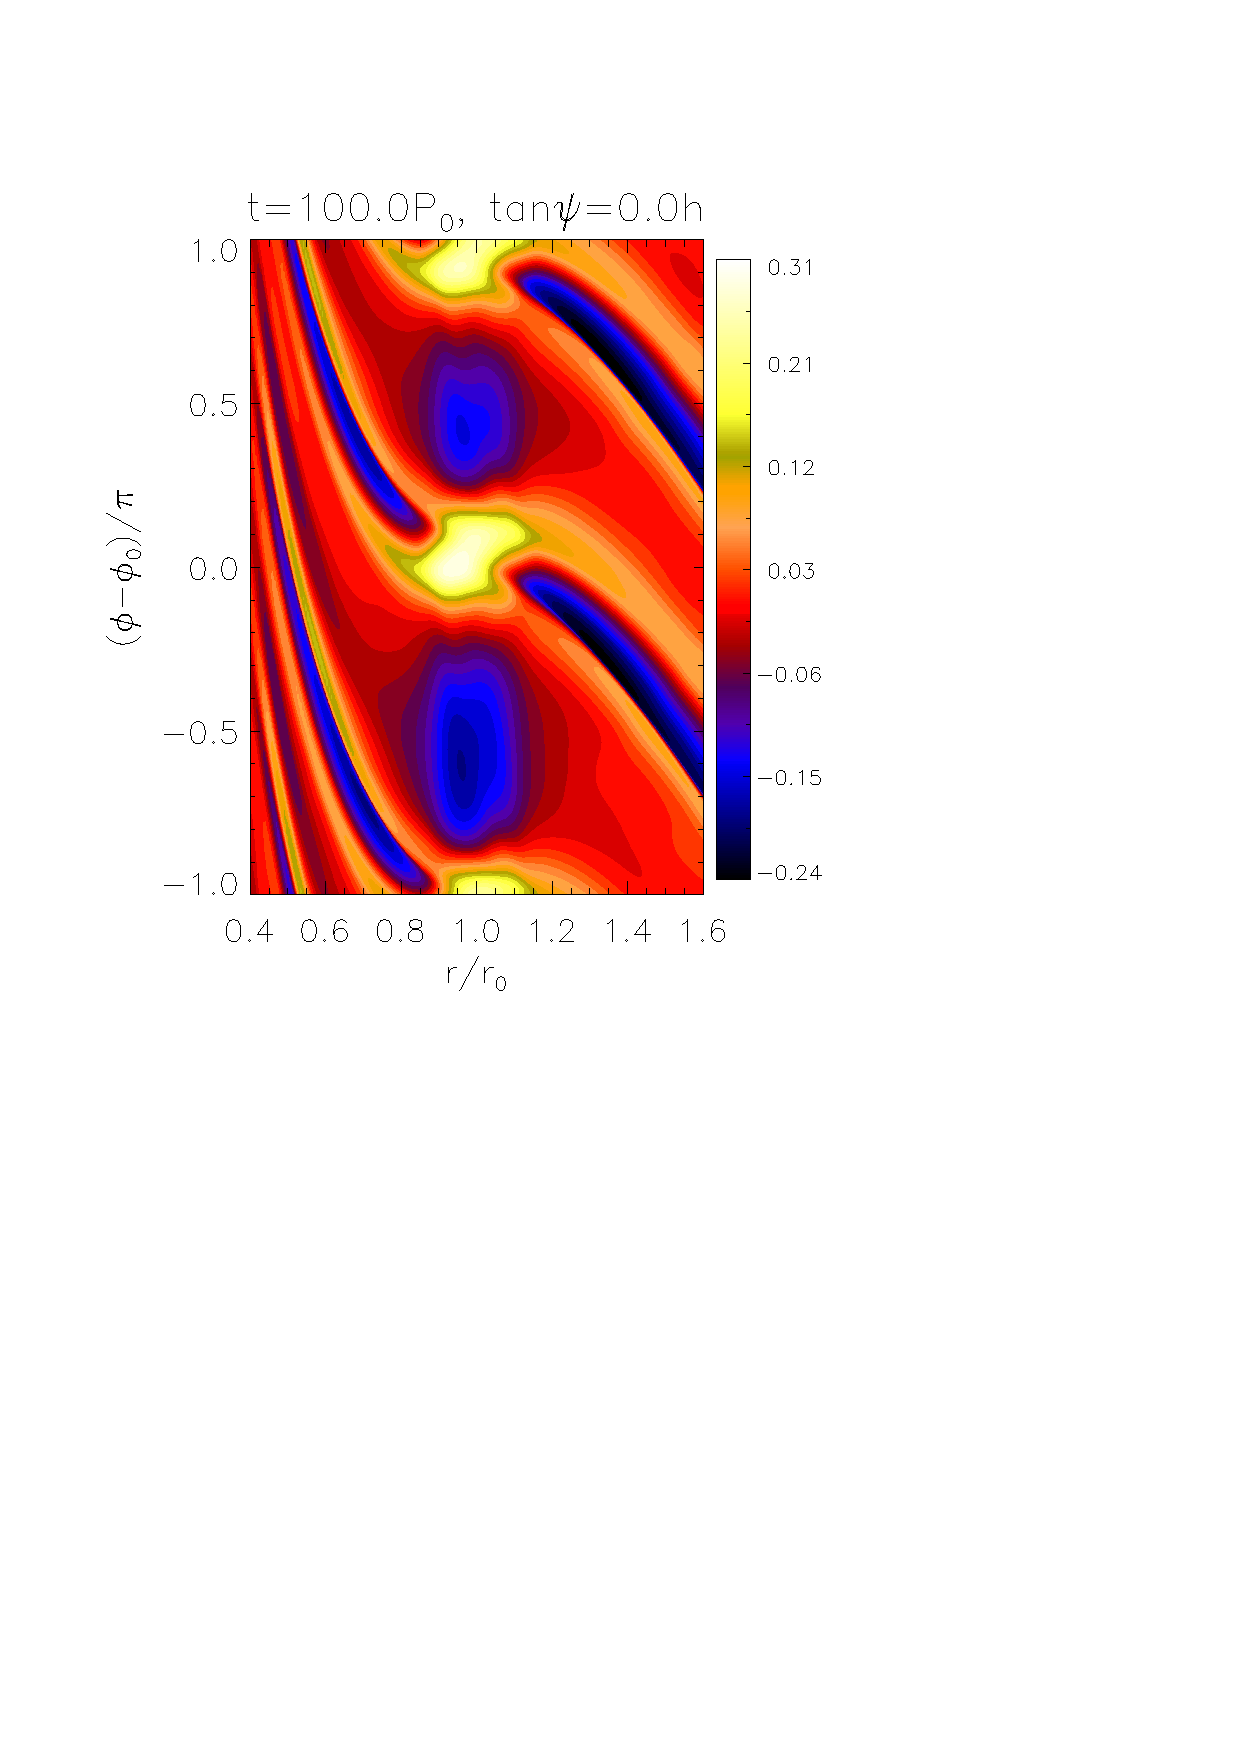
\includegraphics[scale=.27,clip=true,trim=2.3cm
     0cm 0cm
     0cm]{figures/vdamp3_pdisk019}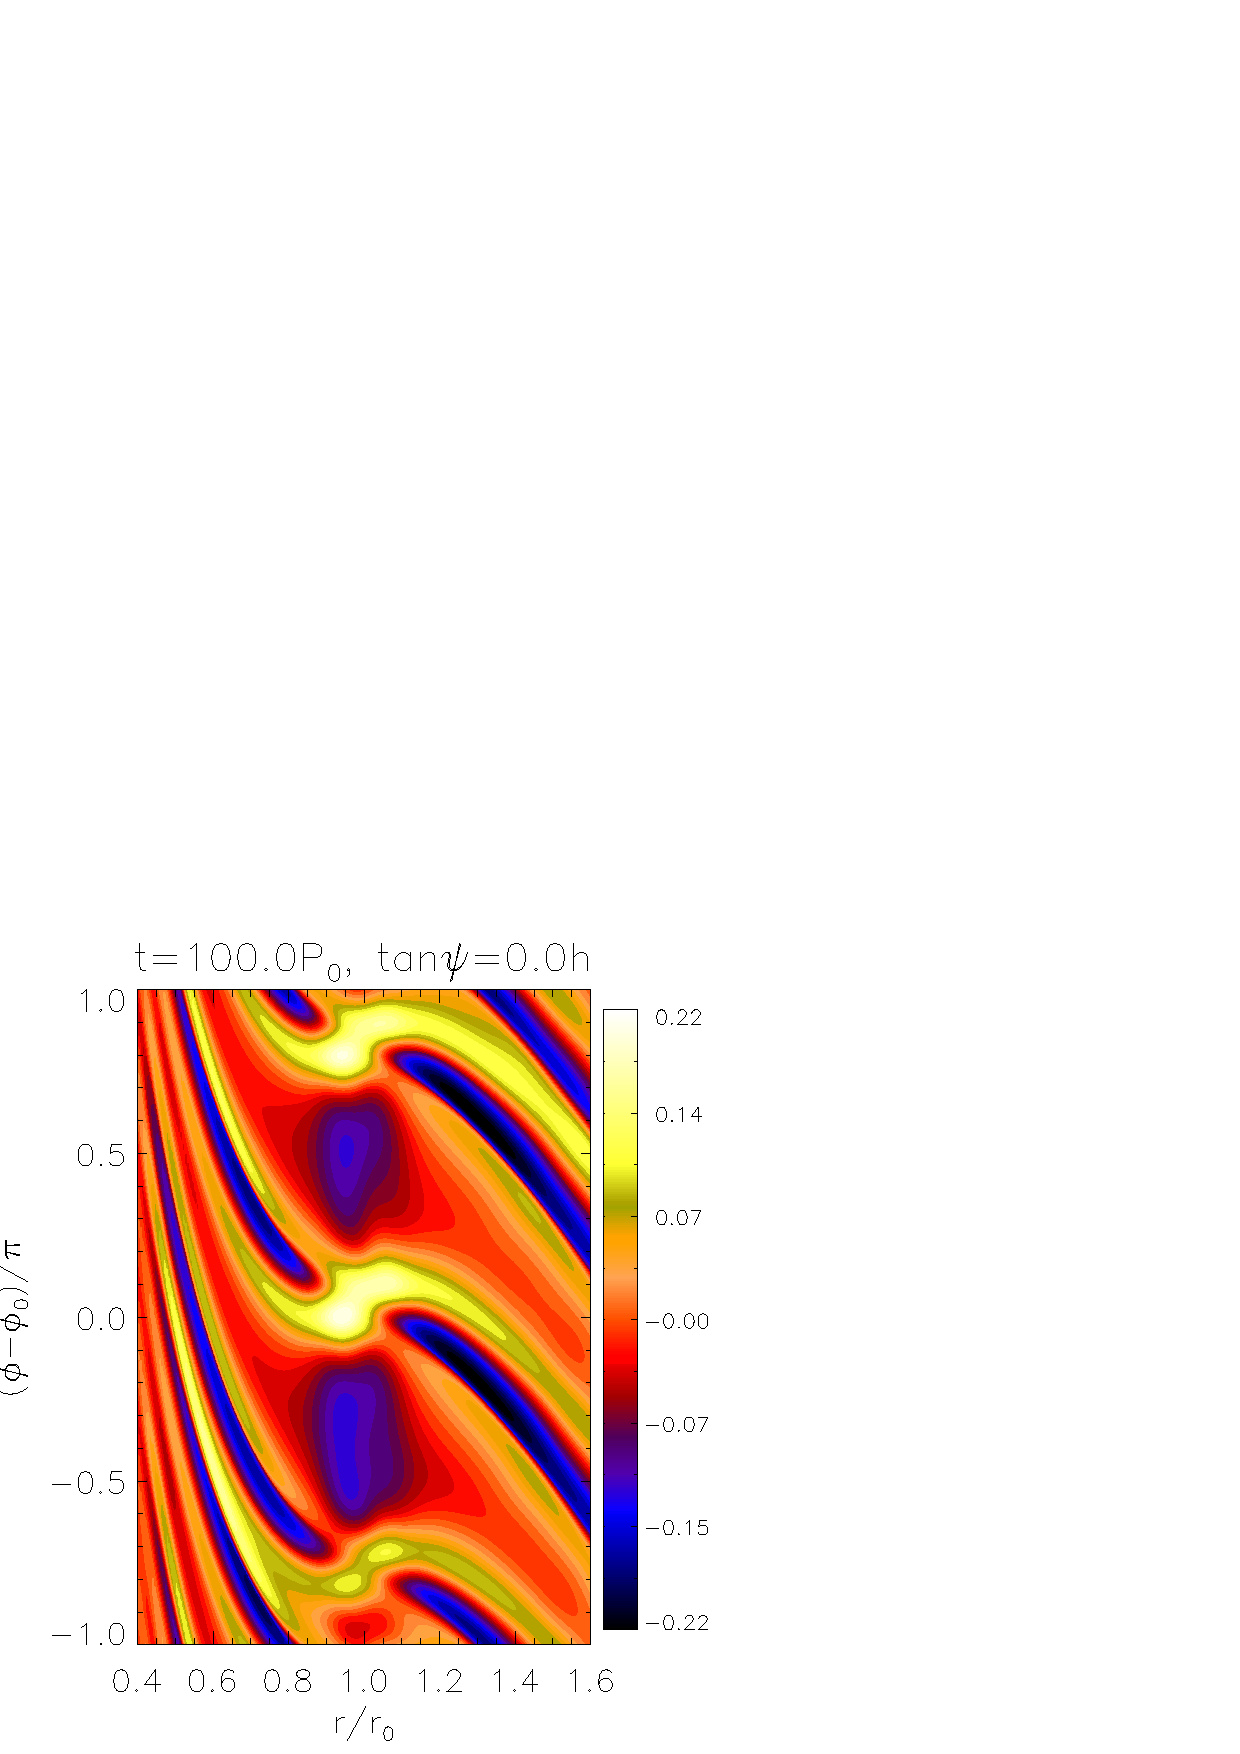
\includegraphics[scale=.27,clip=true,clip=true,trim=2.3cm
     0cm 0cm
     0cm]{figures/vdamp0_nu4_pdisk019}%% \\
   %% 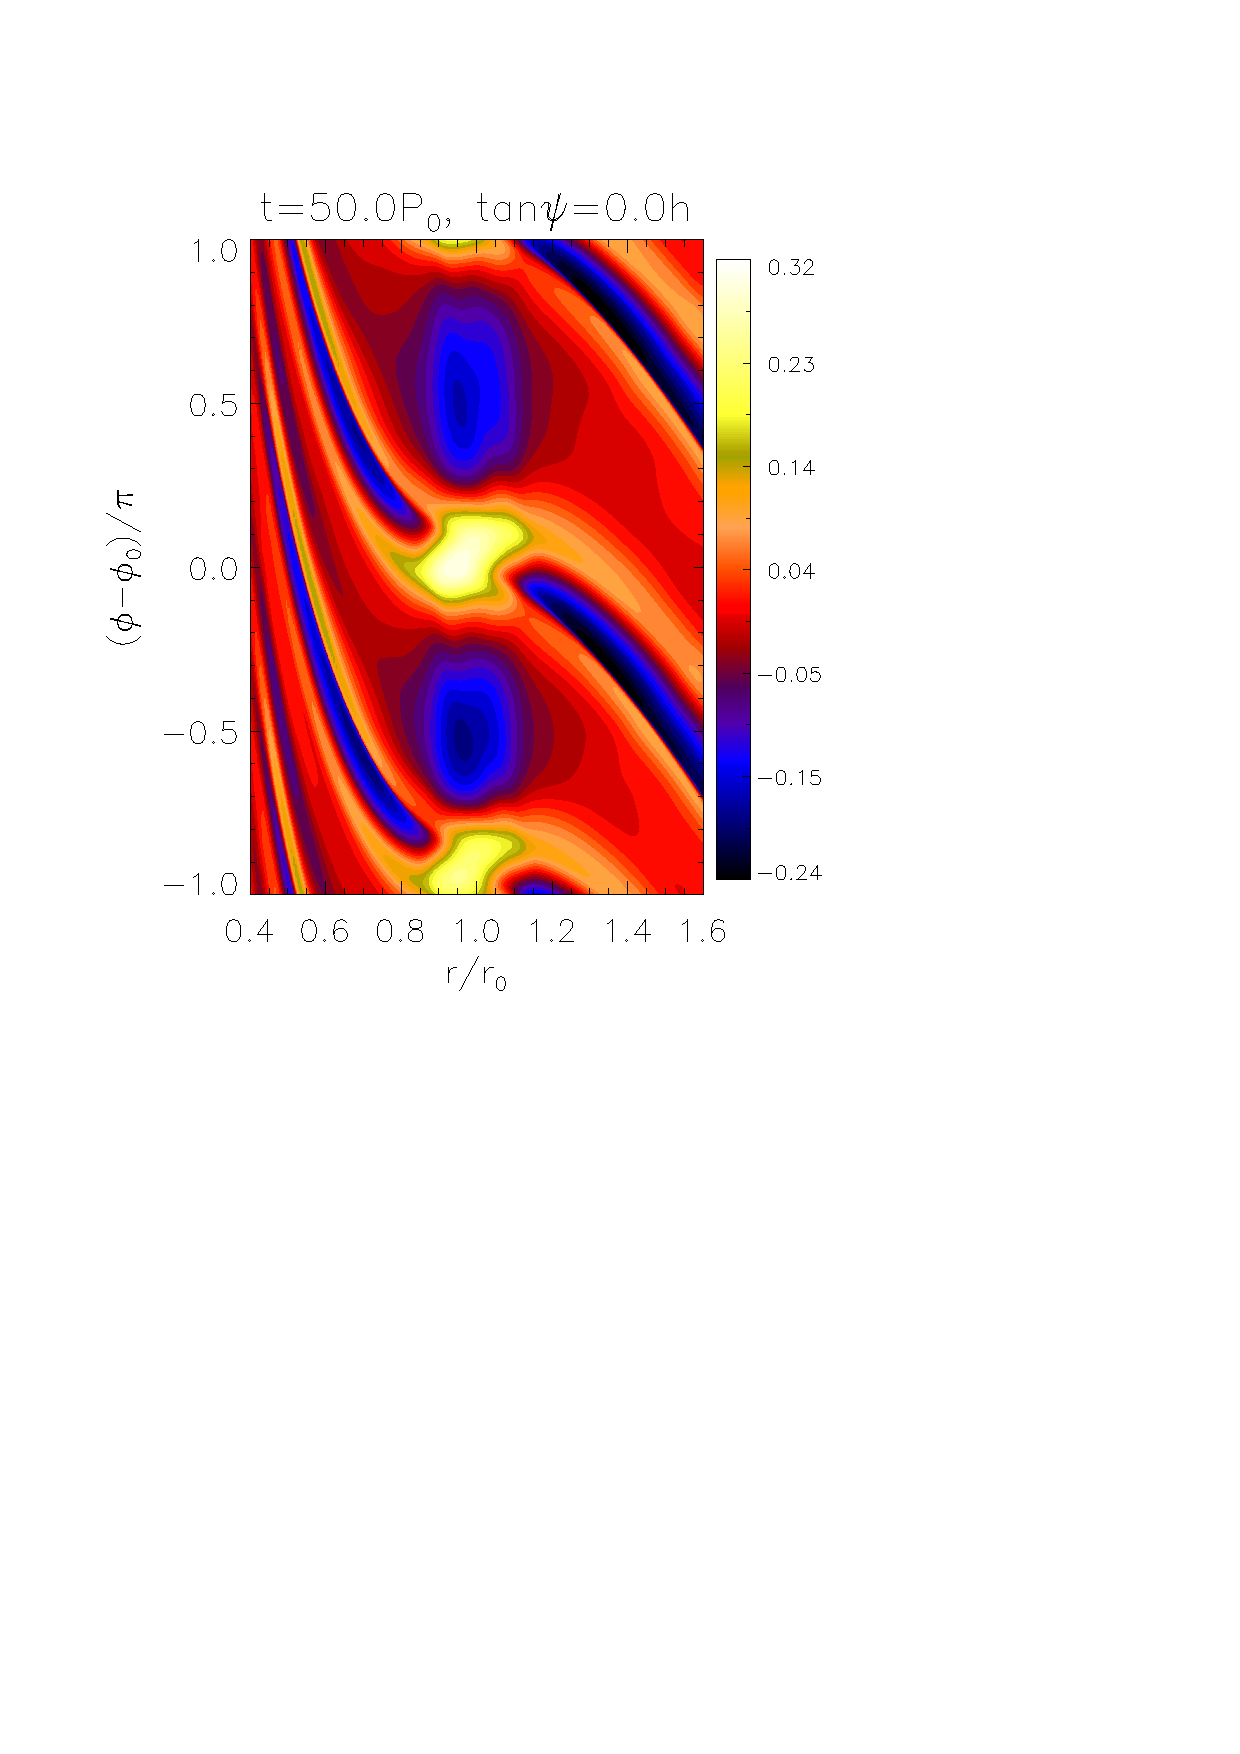
\includegraphics[scale=.27,clip=true,trim=0cm 1.84cm 0.0cm
   %%   0.99cm]{figures/vdamp3_pdisk014}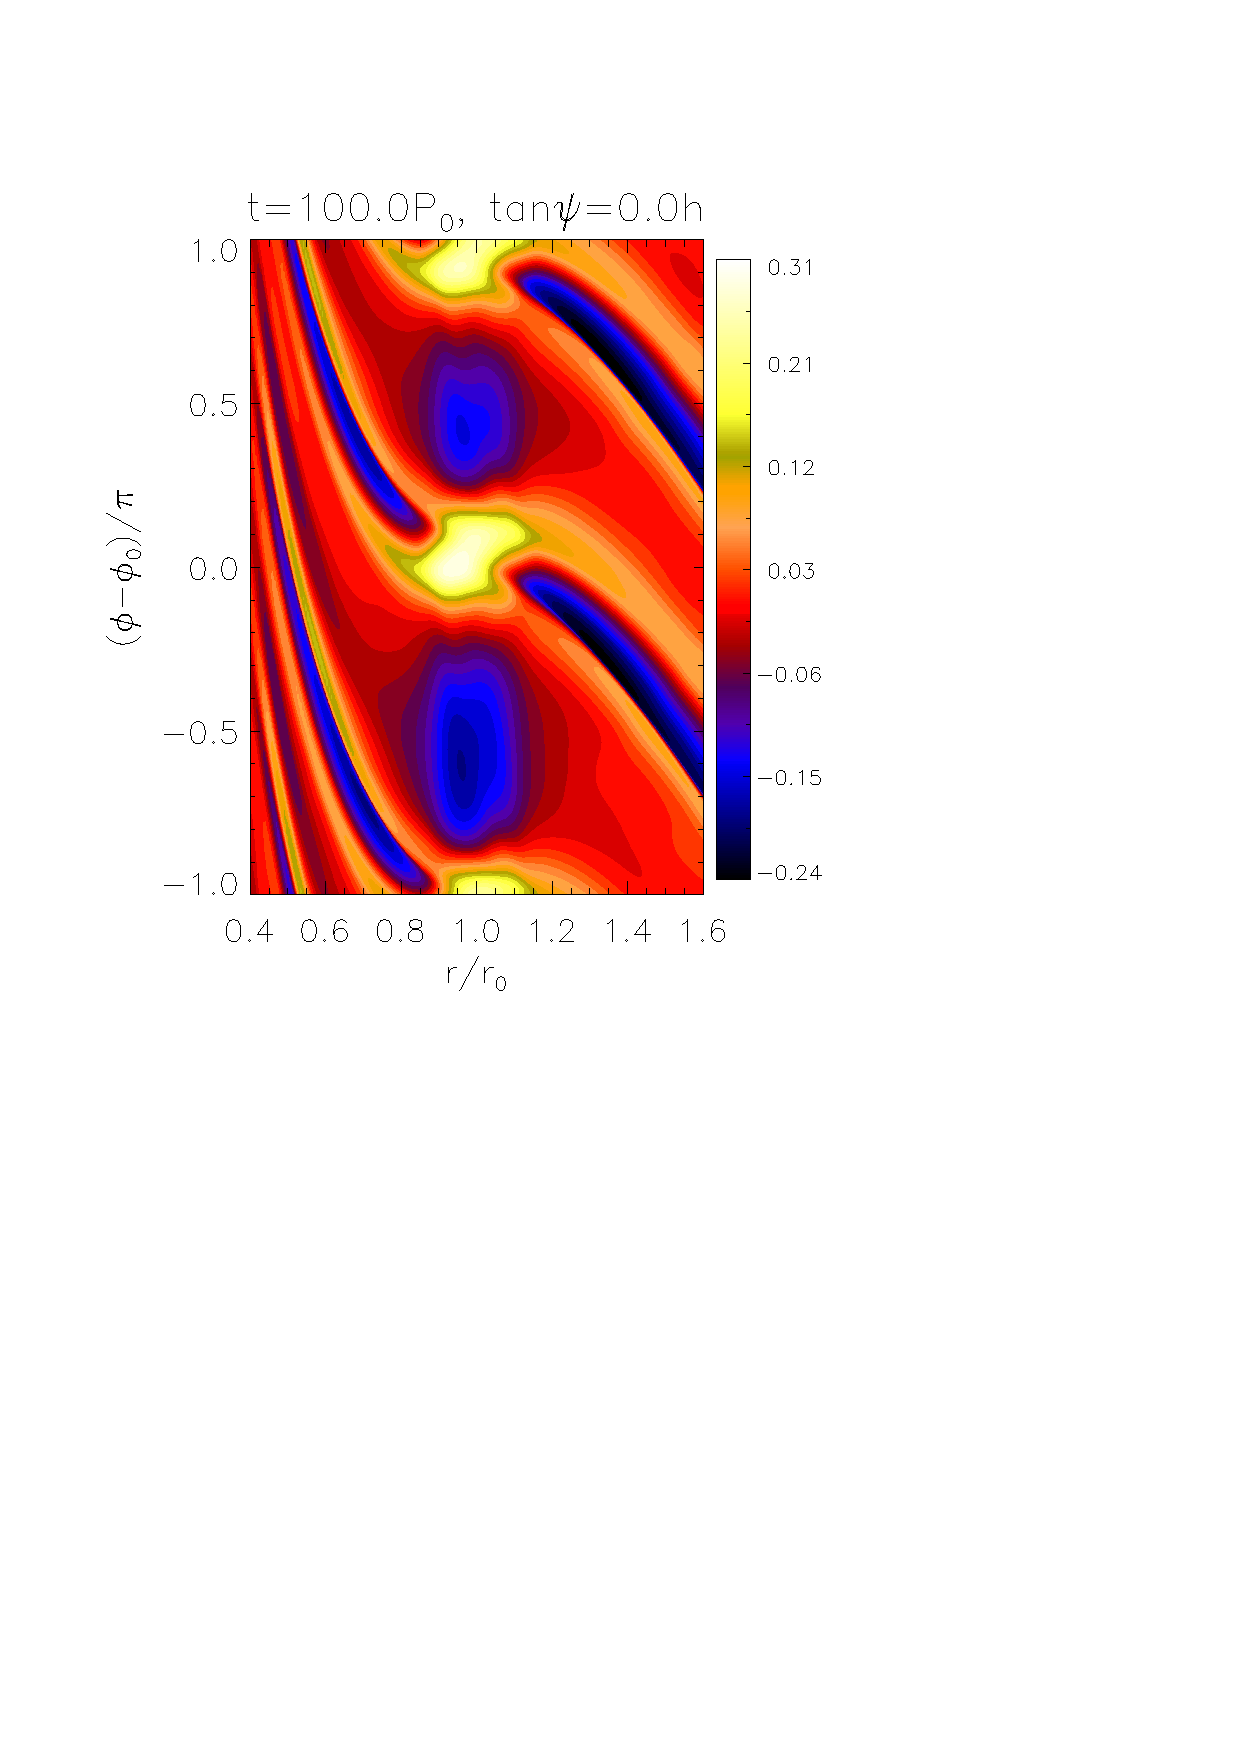
\includegraphics[scale=.27,clip=true,trim=2.3cm
   %%   1.84cm 0.cm
   %%   0.99cm]{figures/vdamp3_pdisk019}\includegraphics[scale=.27,clip=true,clip=true,trim=2.3cm
   %%   1.84cm 0.cm
   %%    0.99cm]{figures/vdamp3_pdisk024}\\
   %%  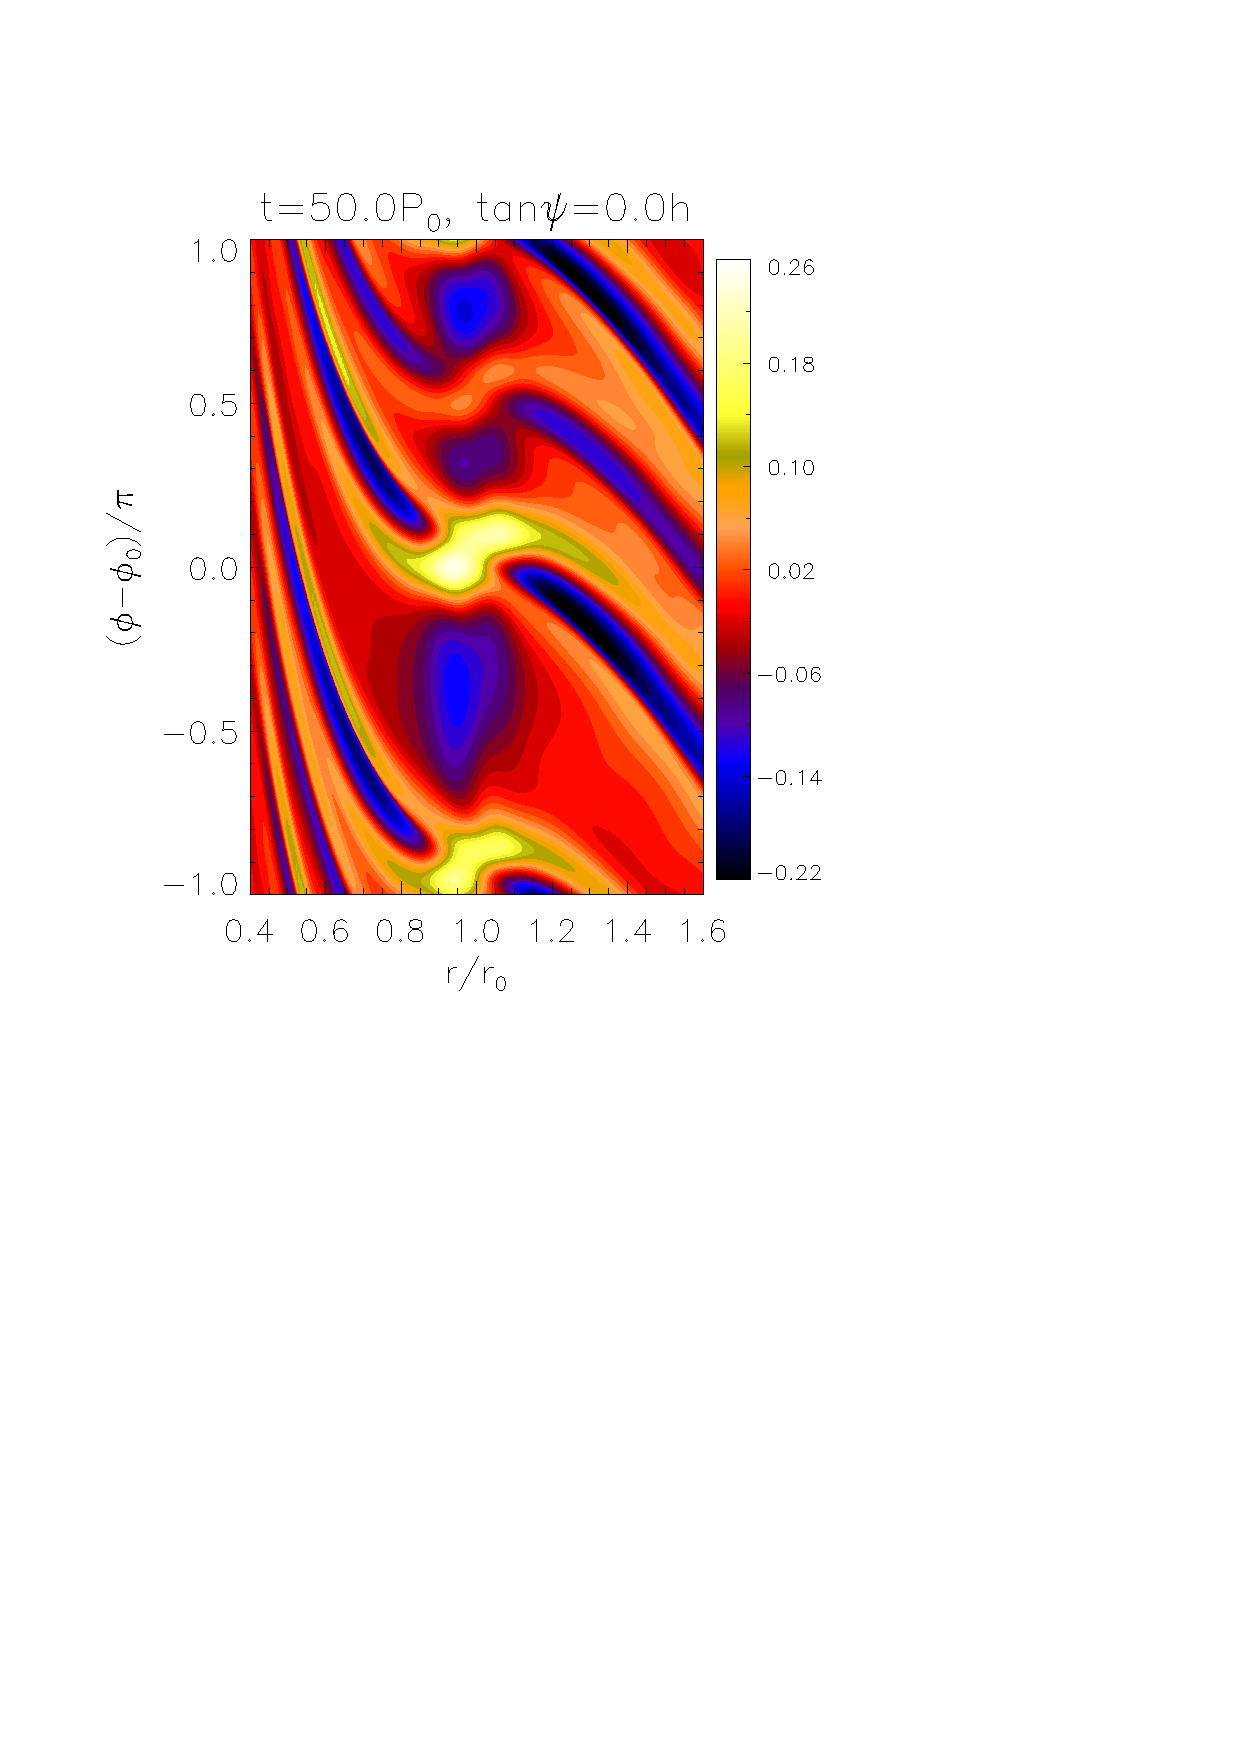
\includegraphics[scale=.27,clip=true,trim=0cm 0.cm 0.0cm
   %%   0.99cm]{figures/vdamp0_nu4_pdisk014}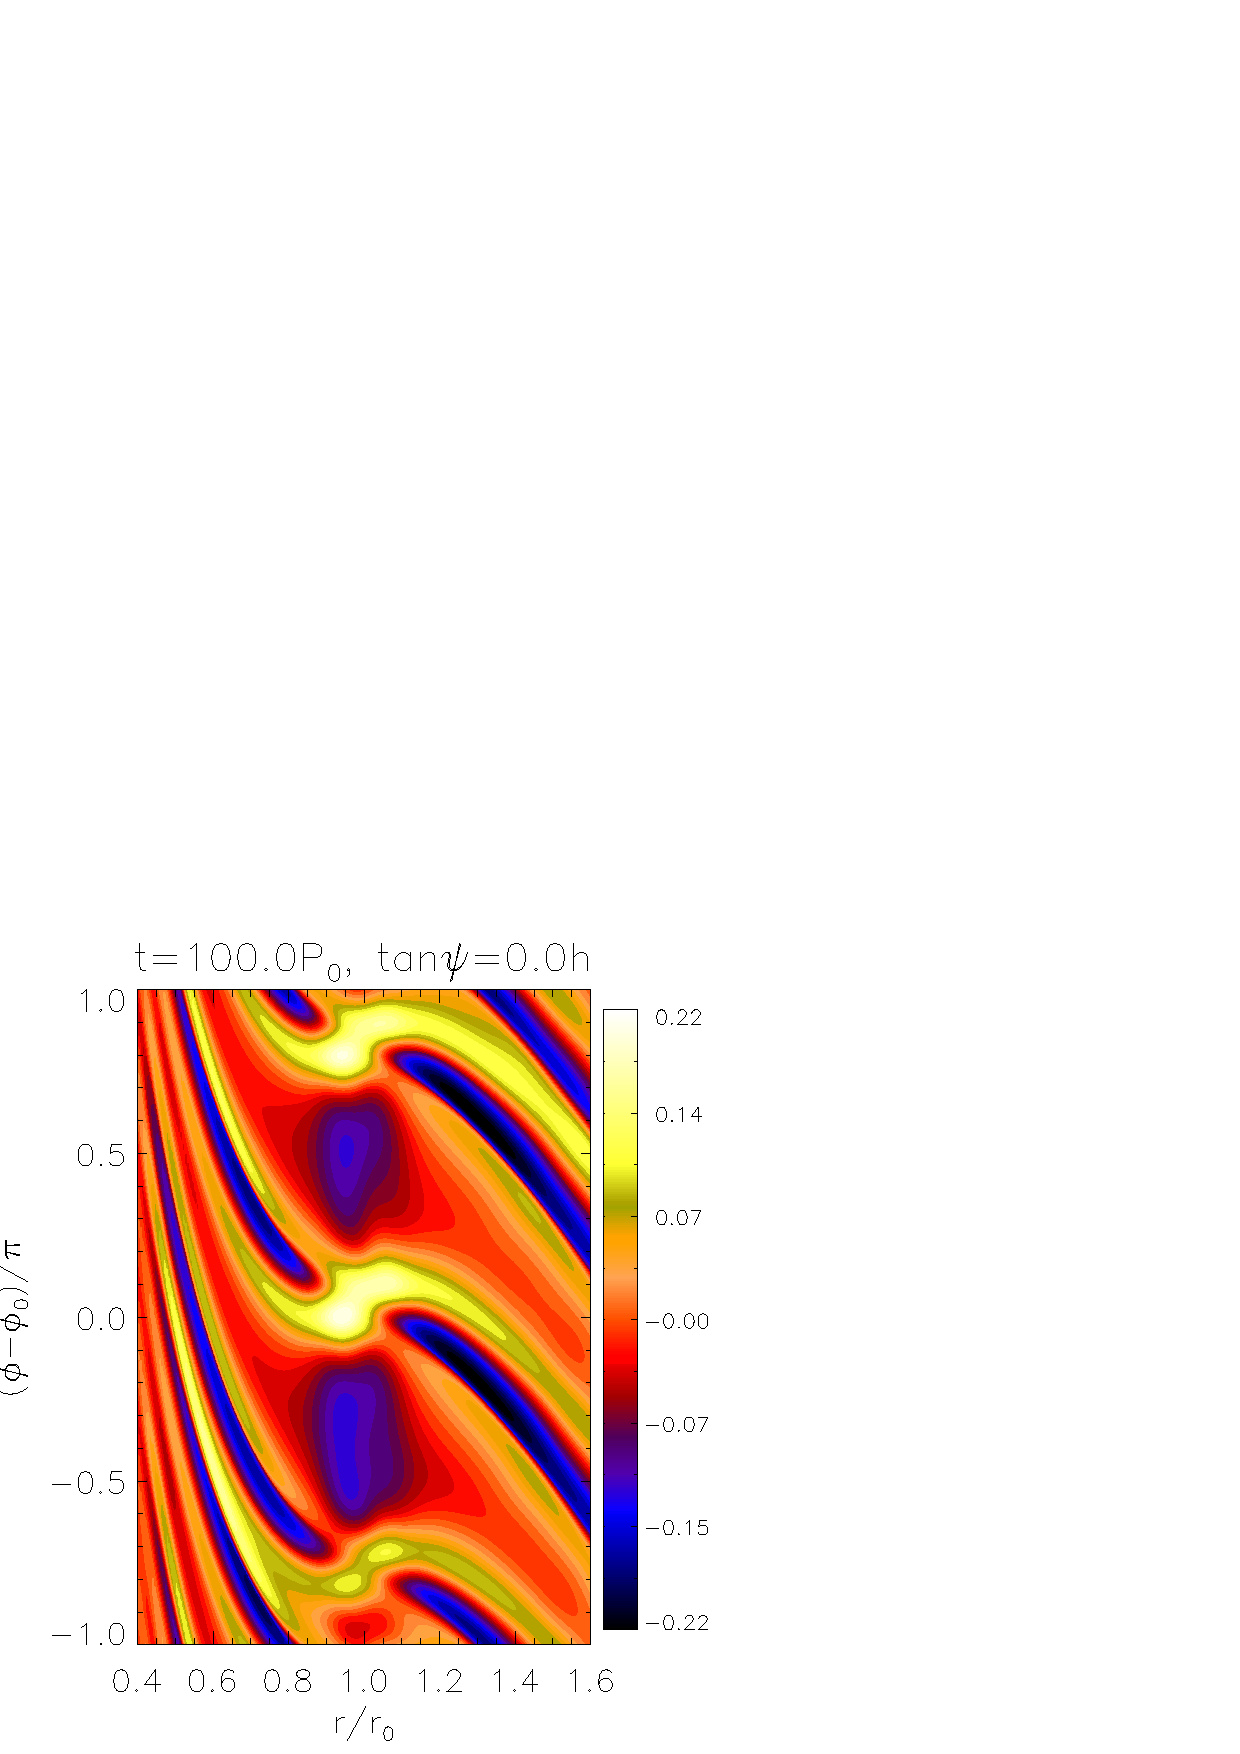
\includegraphics[scale=.27,clip=true,trim=2.3cm
   %%   0.cm 0.cm
   %%   0.99cm]{figures/vdamp0_nu4_pdisk019}\includegraphics[scale=.27,clip=true,clip=true,trim=2.3cm
   %%   0.cm 0.cm
   %%    0.99cm]{figures/vdamp0_nu4_pdisk024}
    \caption{Non-axisymmetric density field at the midplane,
      $\Delta\rho(z=0)$, for case V1 (left), case V2 (middle) and case
      V3. The vertical domain size is $\tan{\psi_\mathrm{max}} = 2h$,
      and the angular thickness of the upper viscous layer at $r=r_0$
      is $0.5h$ (left), $1.0h$ (middle) and $2.0h$ (right).   
      \label{vdamp2}}
\end{figure}


\begin{figure}
   \centering
   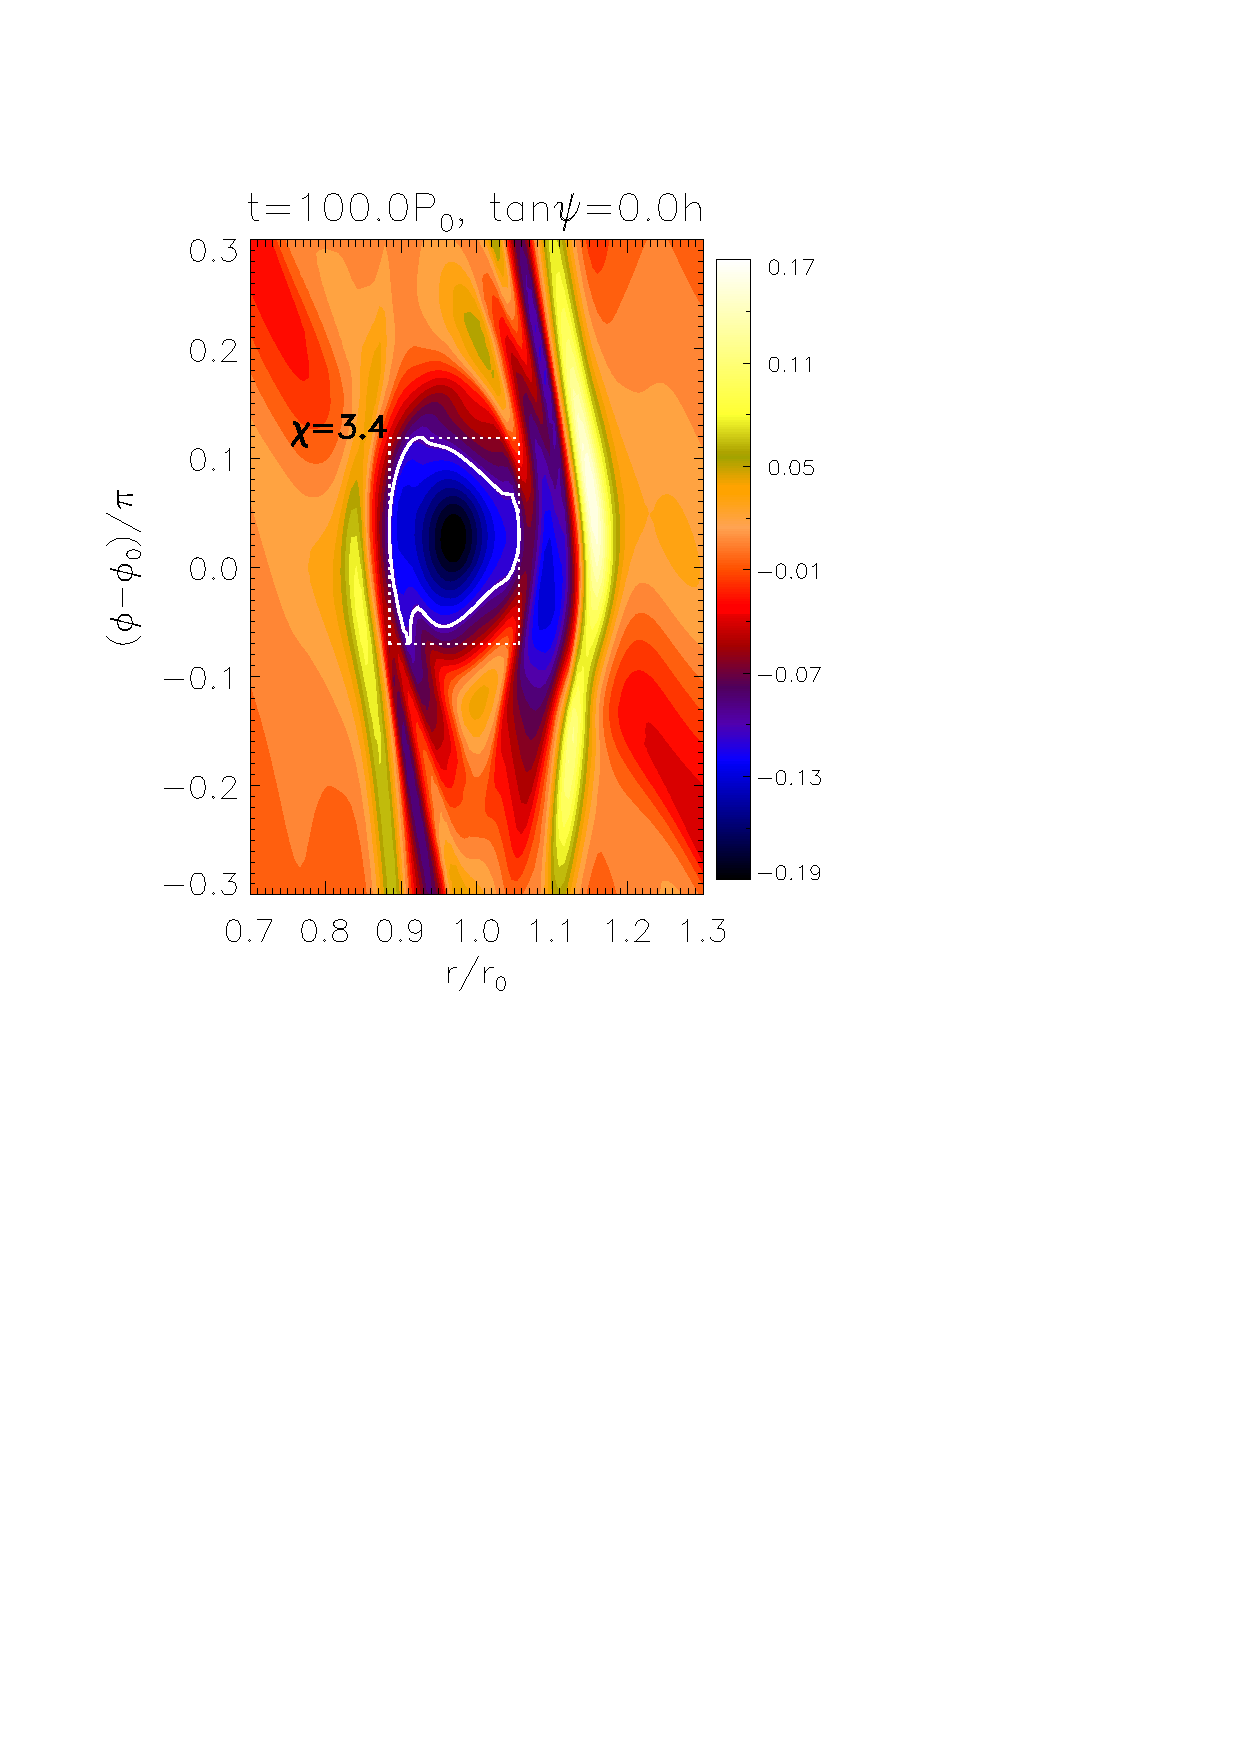
\includegraphics[scale=.27,clip=true,trim=0cm 0cm 0cm
     0cm]{figures/vdamp2_vort019}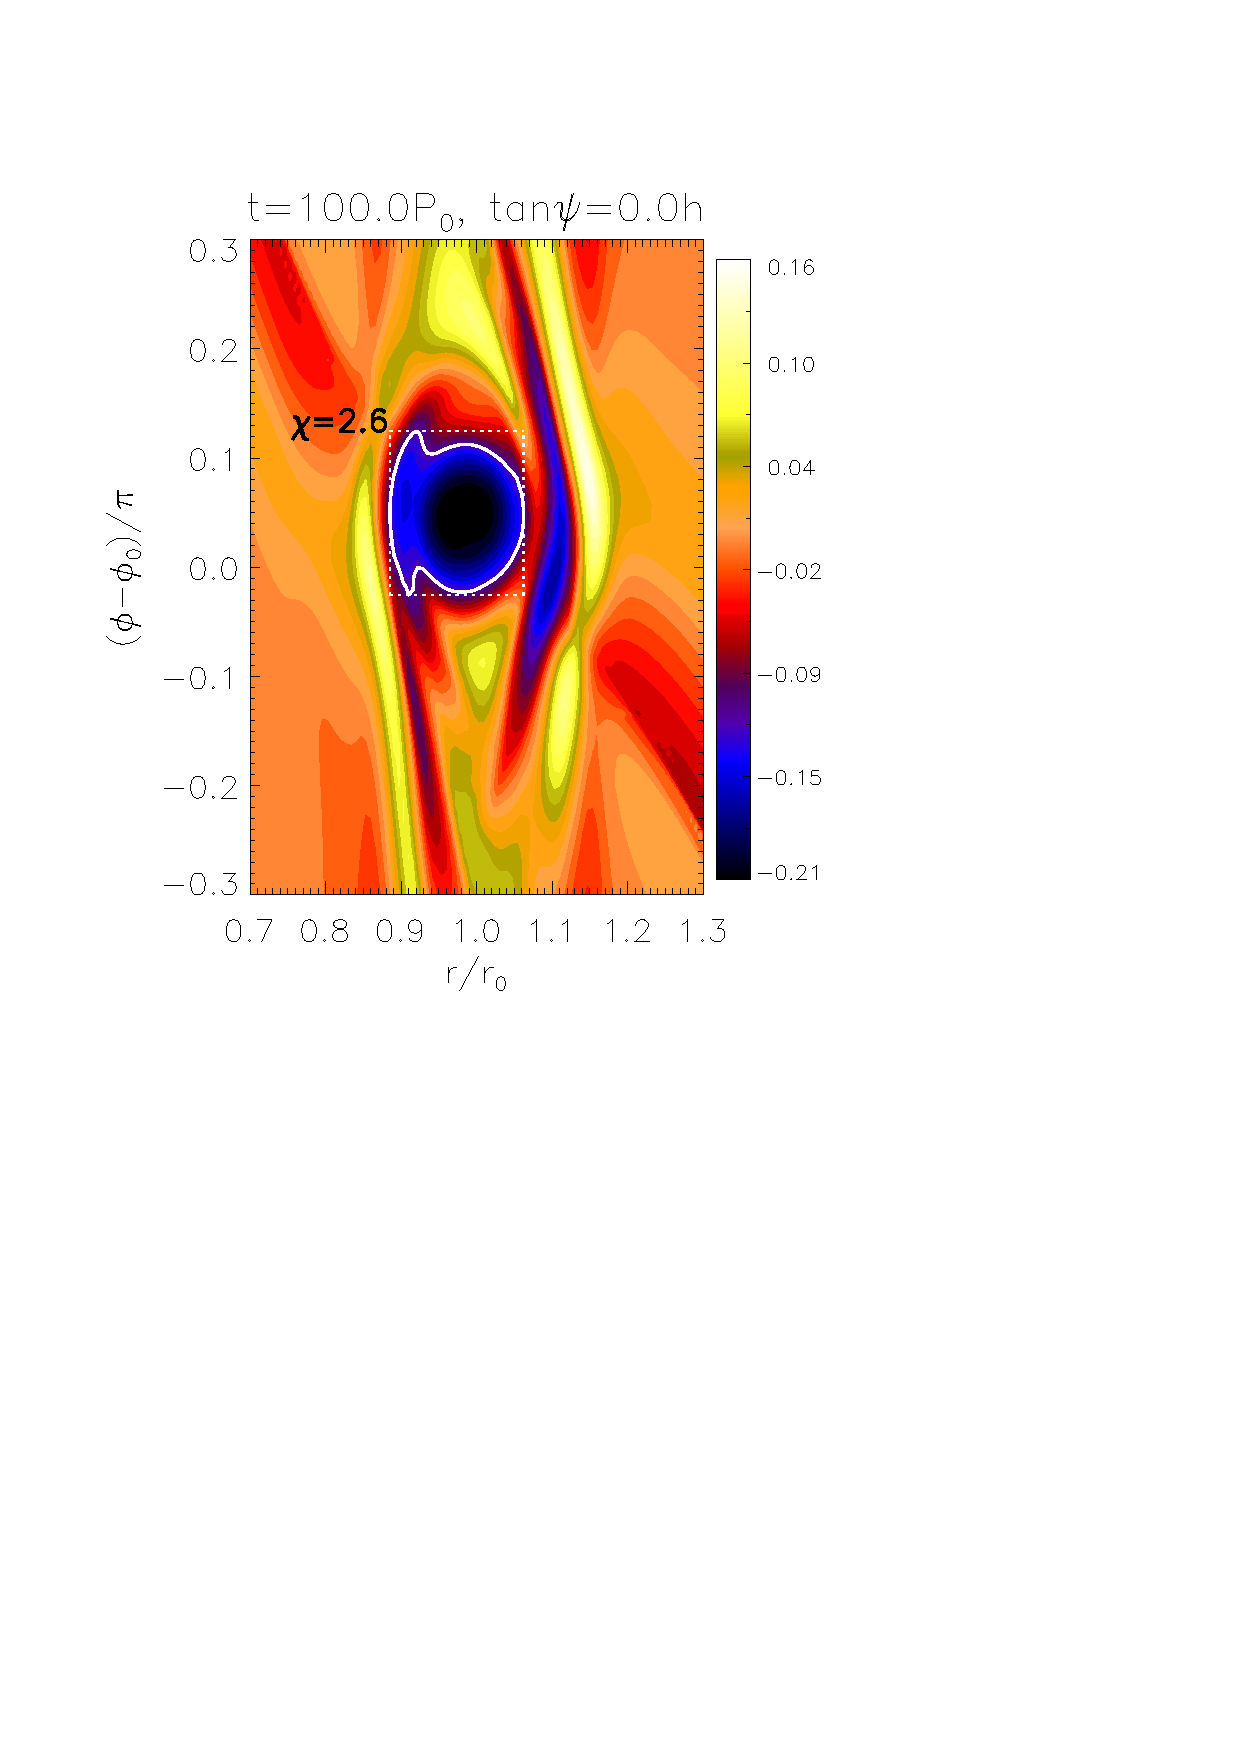
\includegraphics[scale=.27,clip=true,trim=2.3cm
     0cm 0cm
     0cm]{figures/vdamp3_vort019}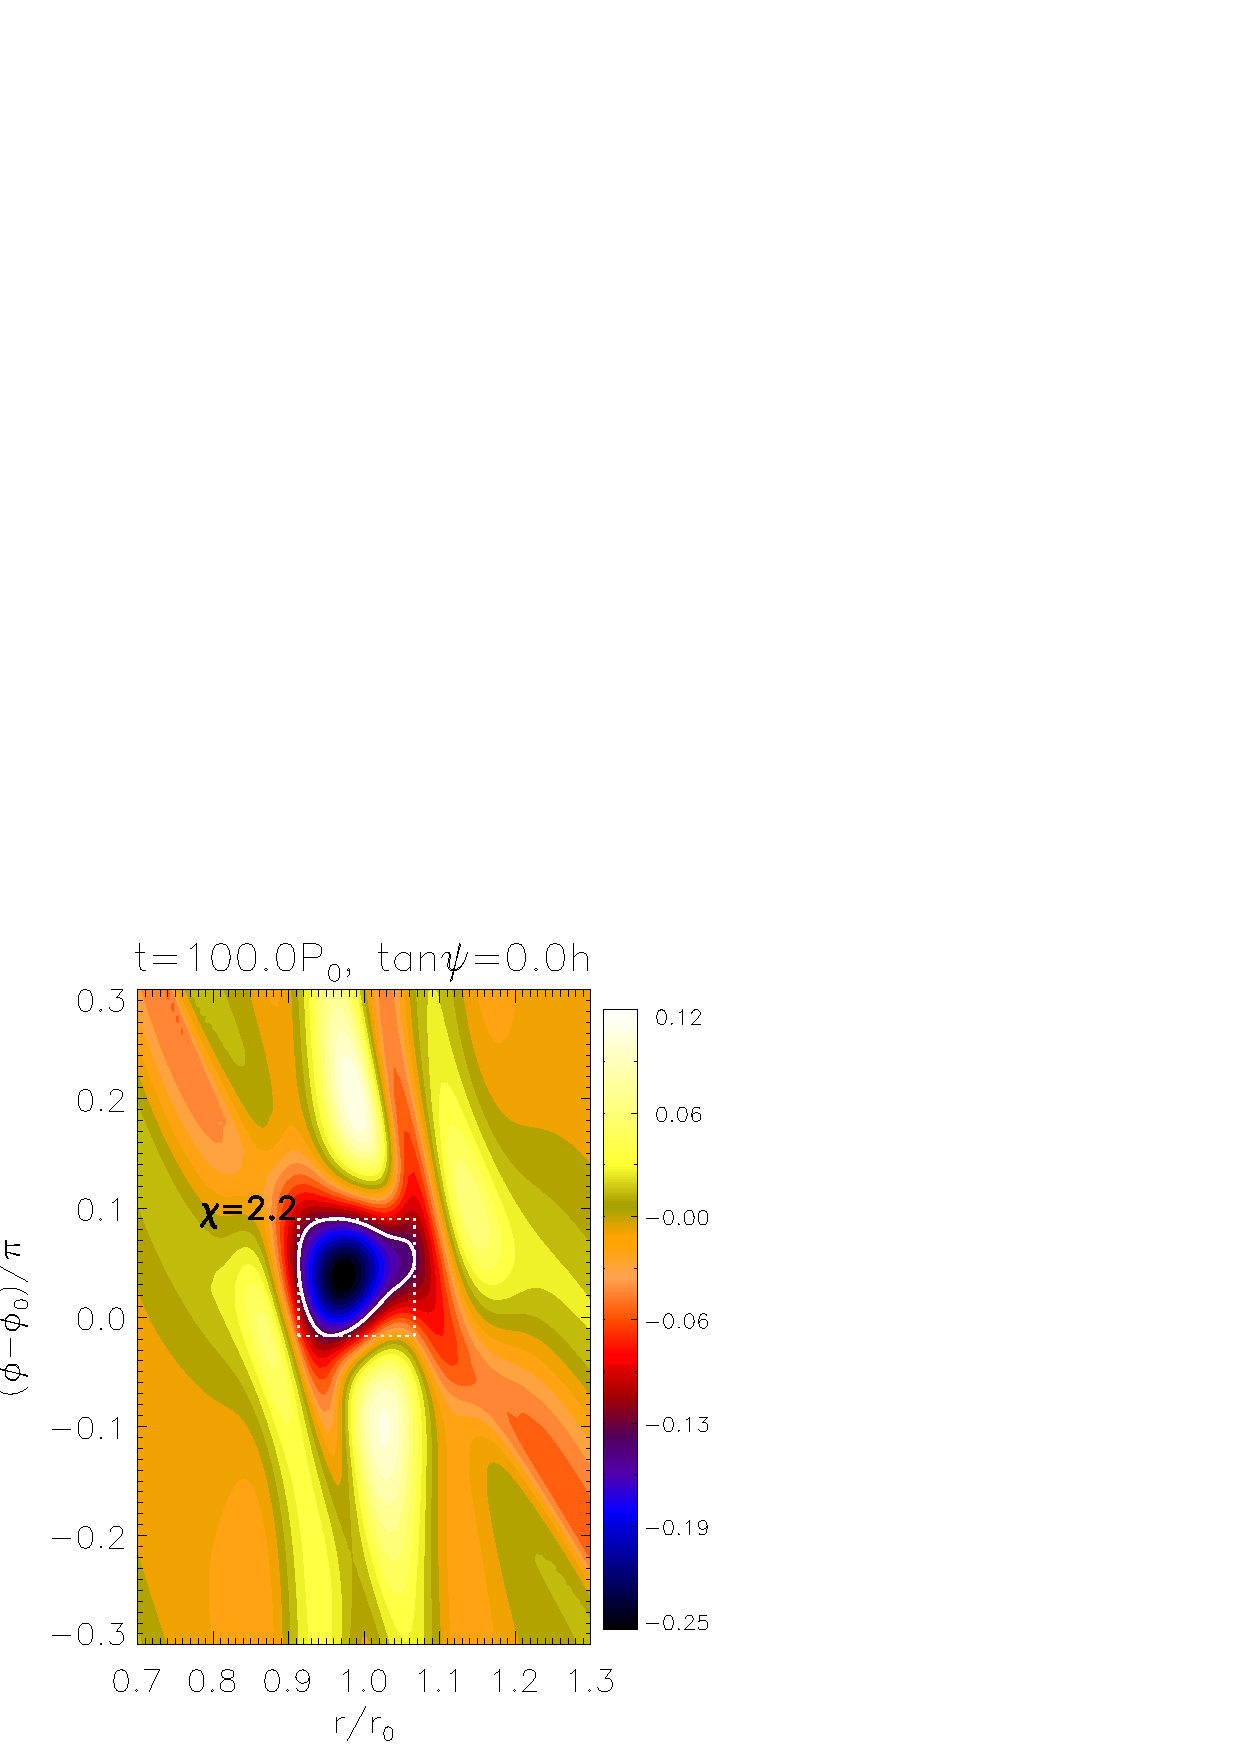
\includegraphics[scale=.27,clip=true,clip=true,trim=2.3cm
     0cm 0cm
     0cm]{figures/vdamp0_nu4_vort019}%% \\
   %% 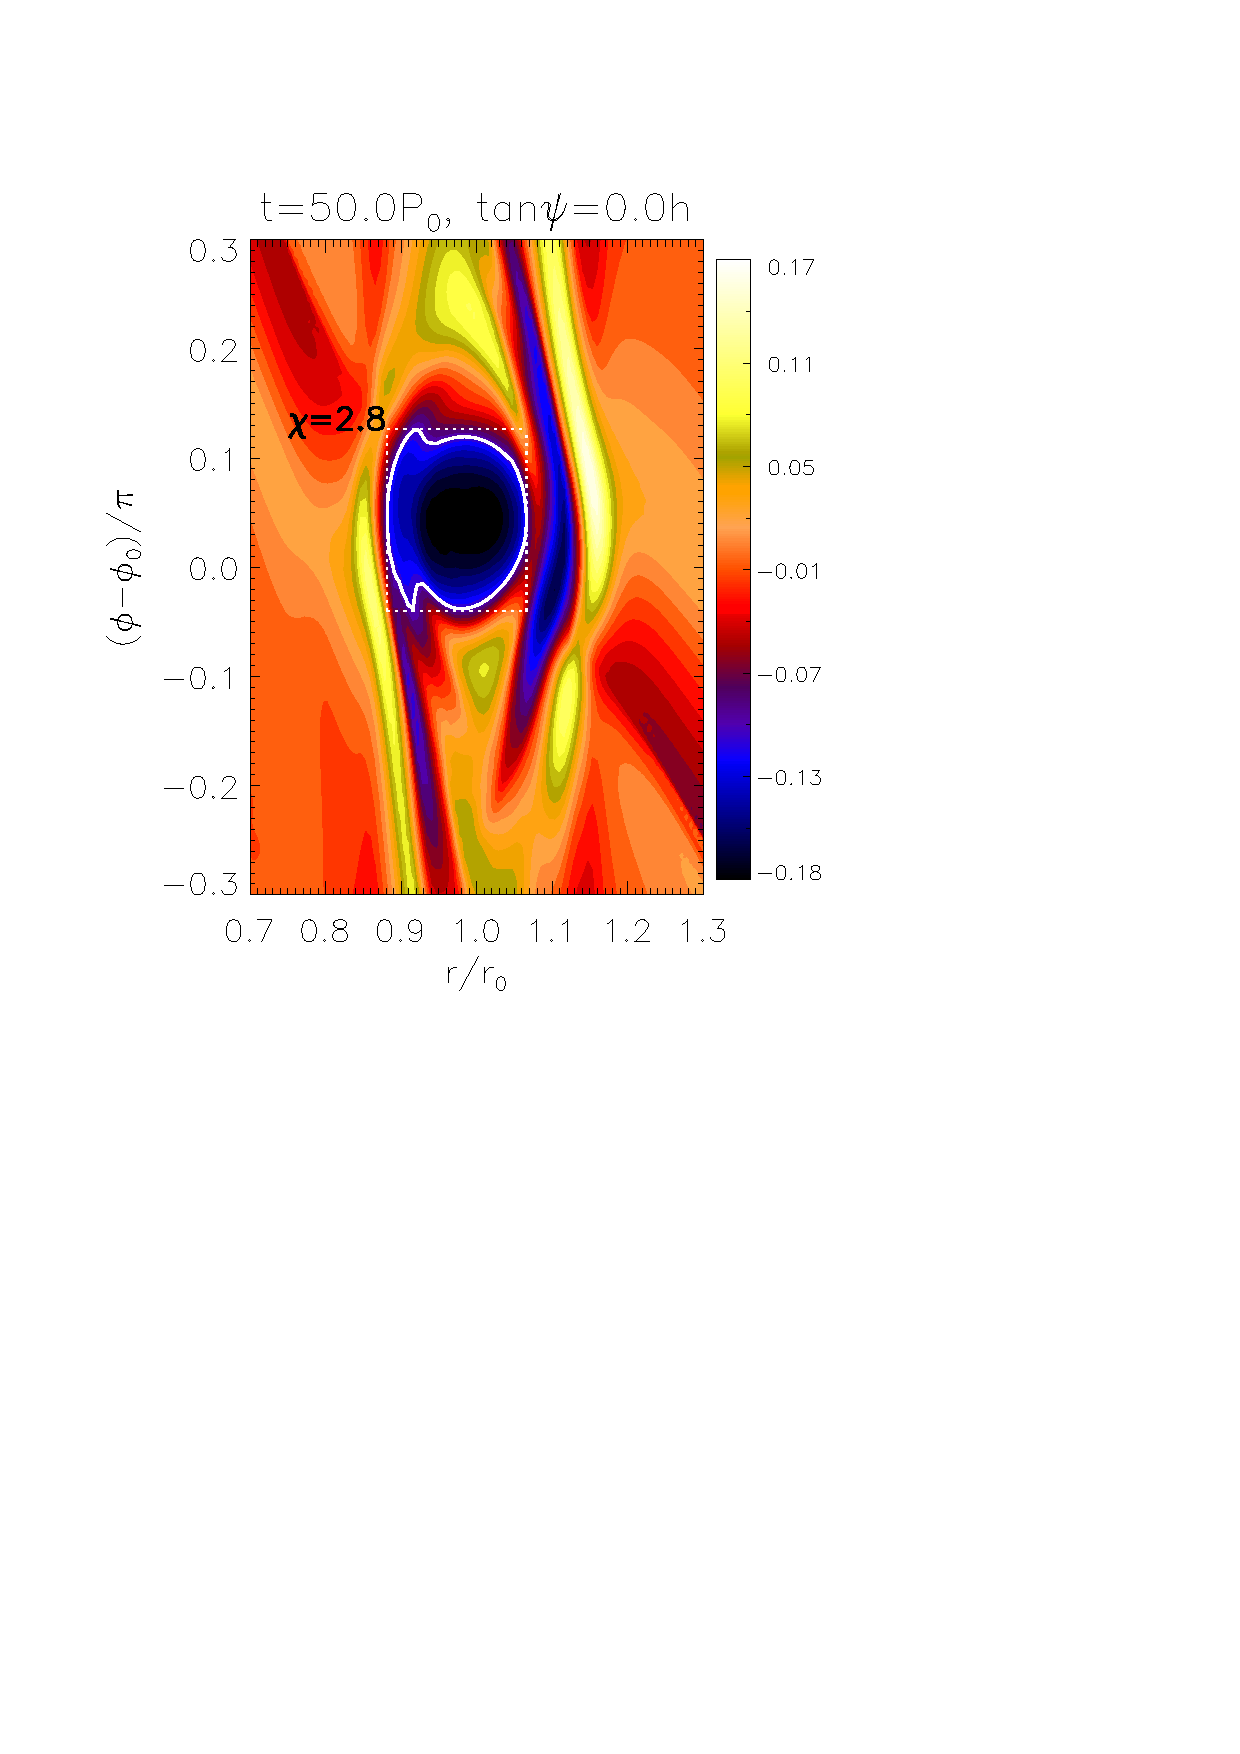
\includegraphics[scale=.27,clip=true,trim=0cm 1.84cm 0.0cm
   %%   0.99cm]{figures/vdamp3_vort014}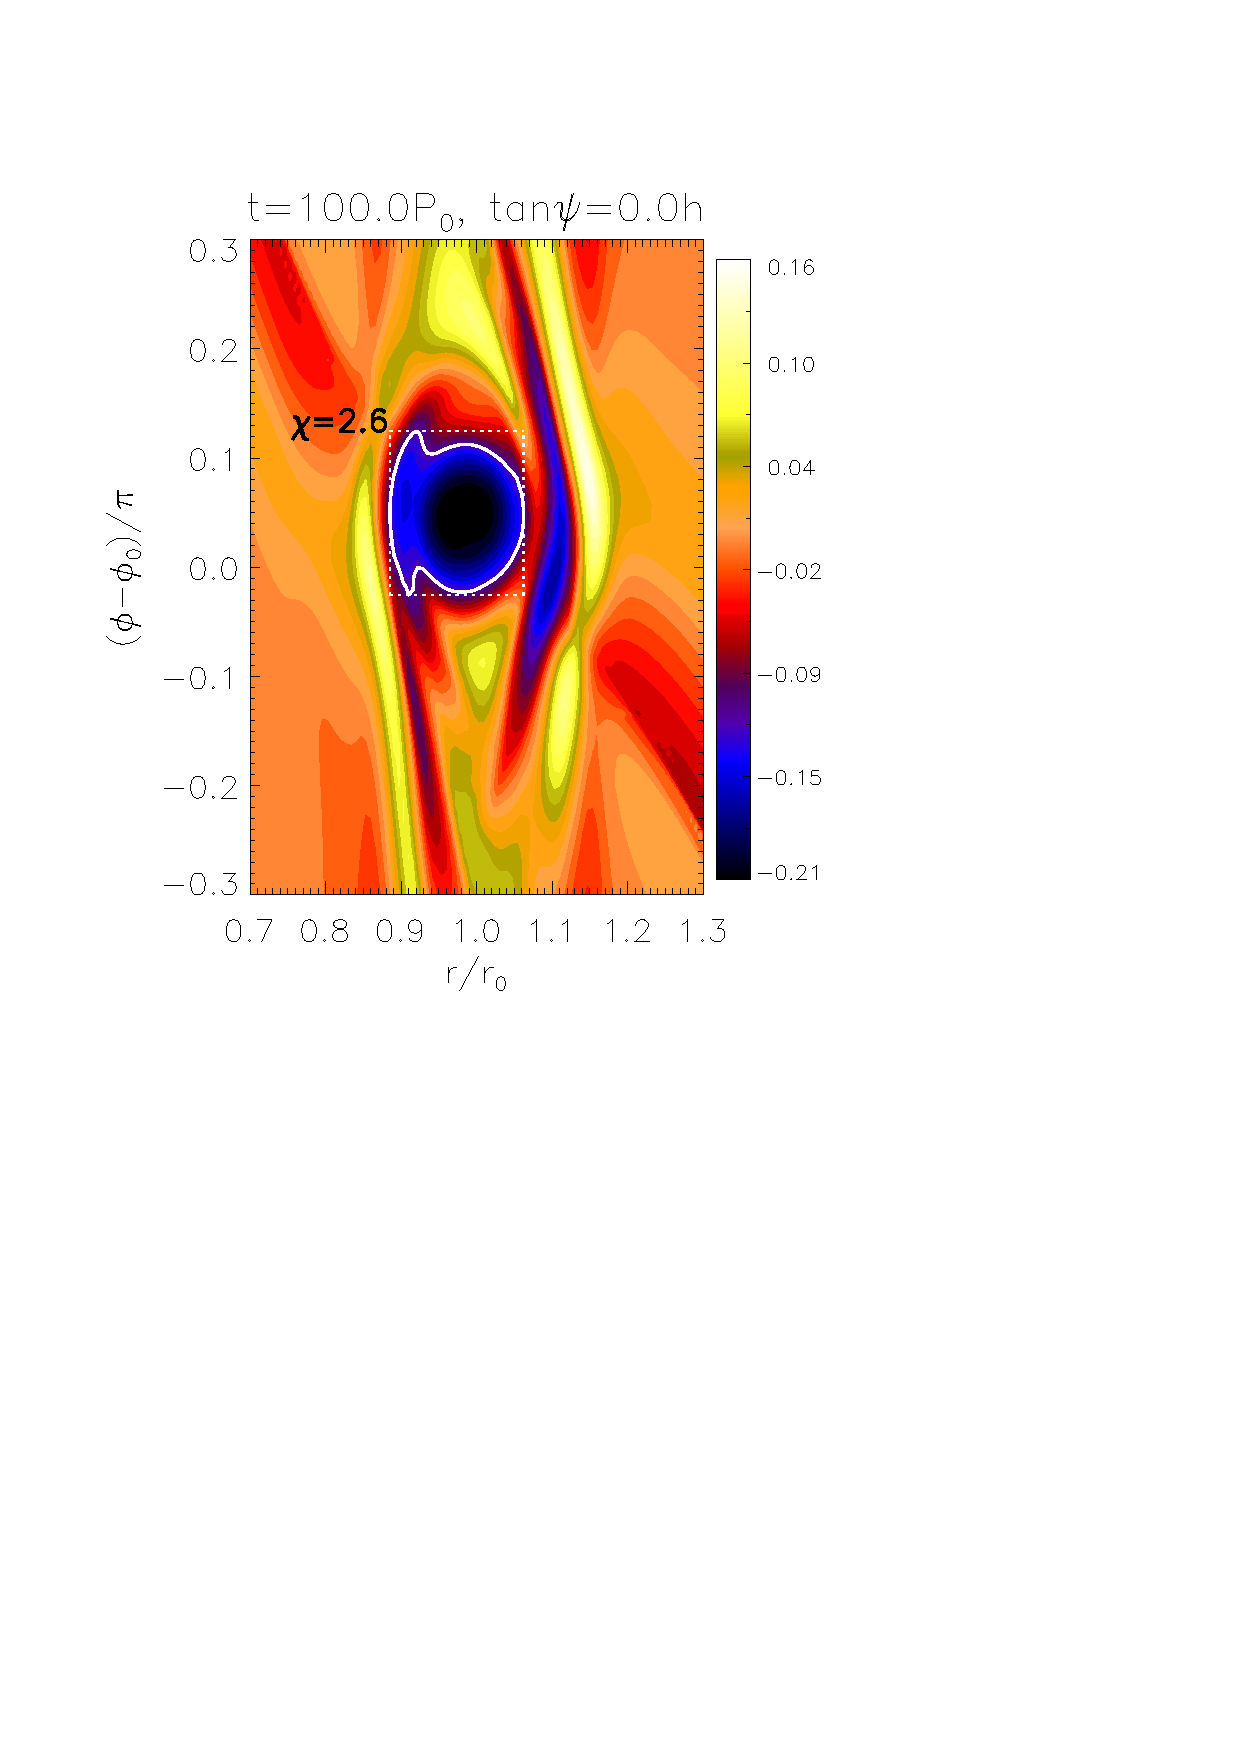
\includegraphics[scale=.27,clip=true,trim=2.3cm
   %%   1.84cm 0.cm
   %%   0.99cm]{figures/vdamp3_vort019}\includegraphics[scale=.27,clip=true,clip=true,trim=2.3cm
   %%   1.84cm 0.cm
   %%    0.99cm]{figures/vdamp3_vort024}\\
   %%  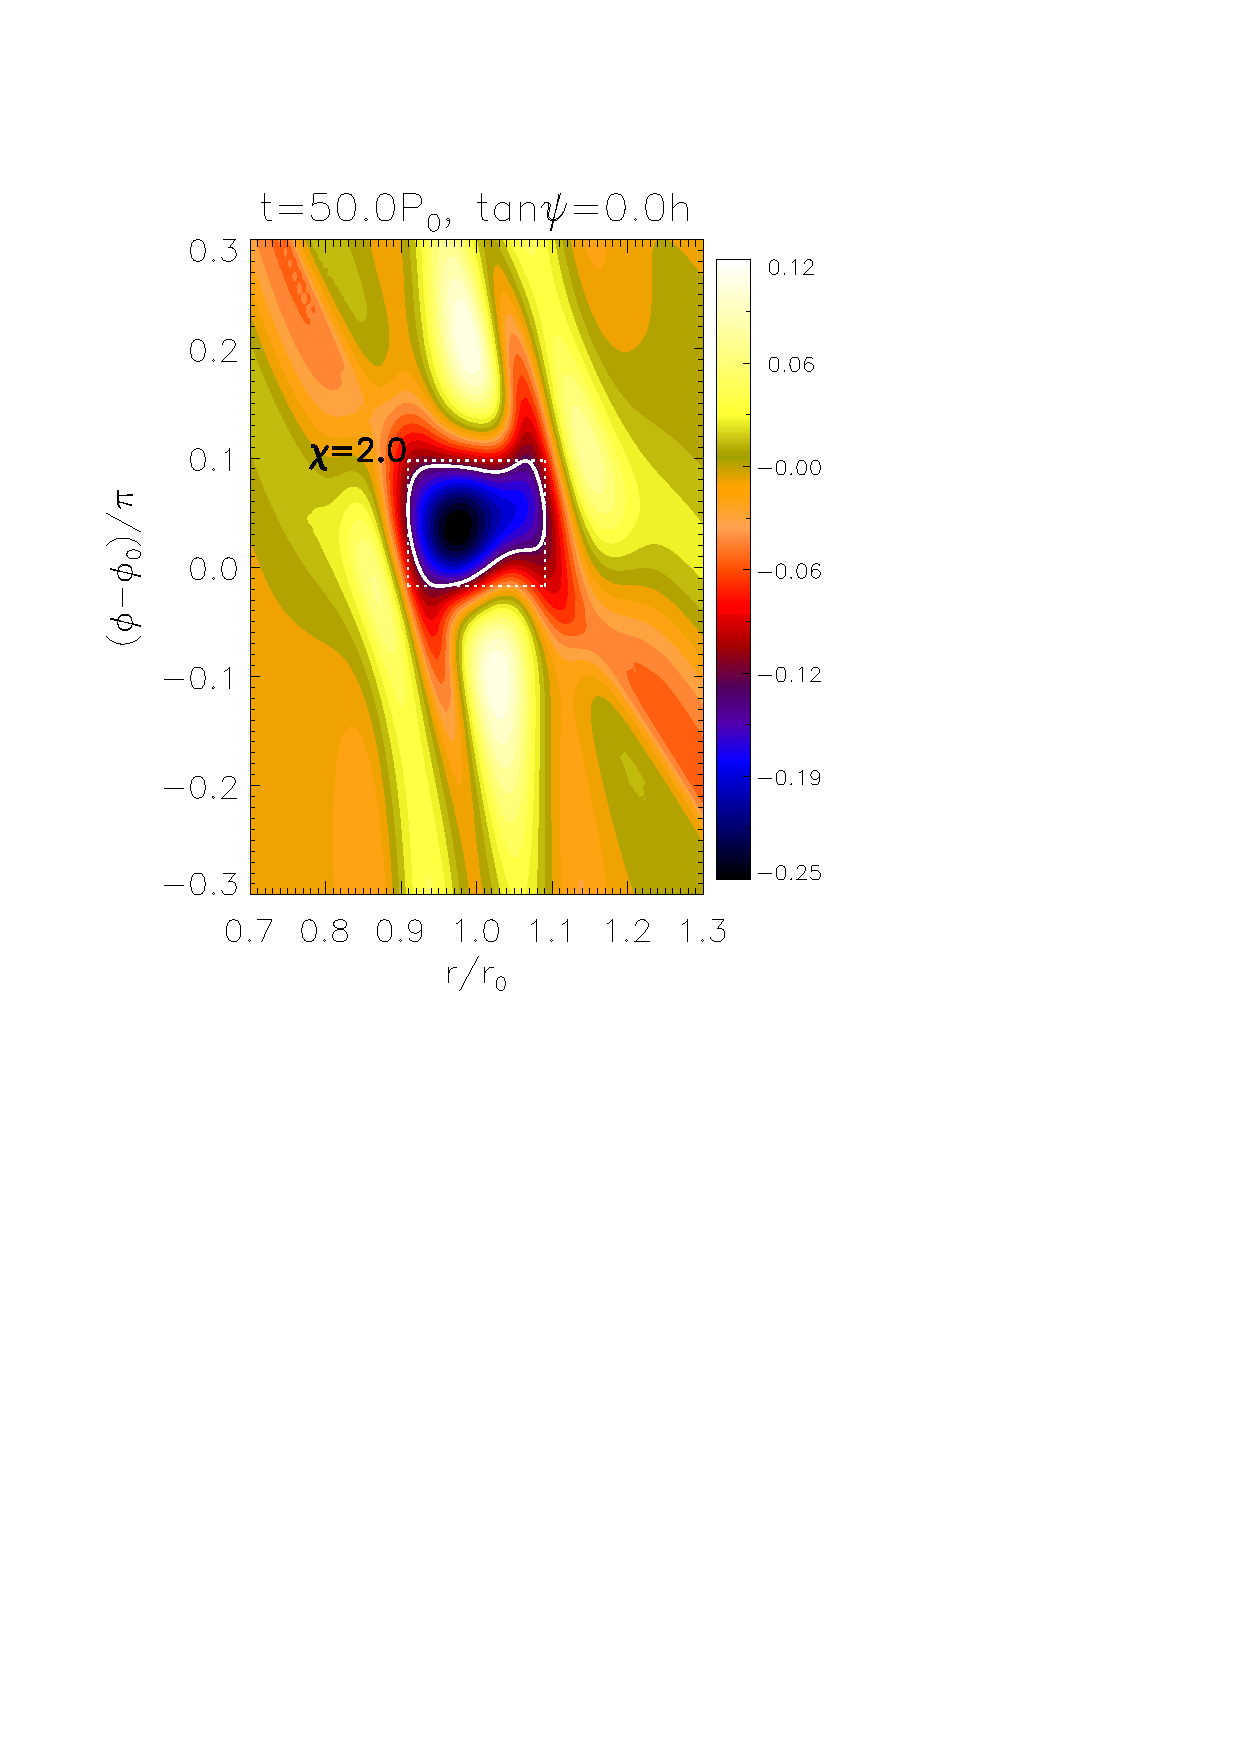
\includegraphics[scale=.27,clip=true,trim=0cm 0.cm 0.0cm
   %%   0.99cm]{figures/vdamp0_nu4_vort014}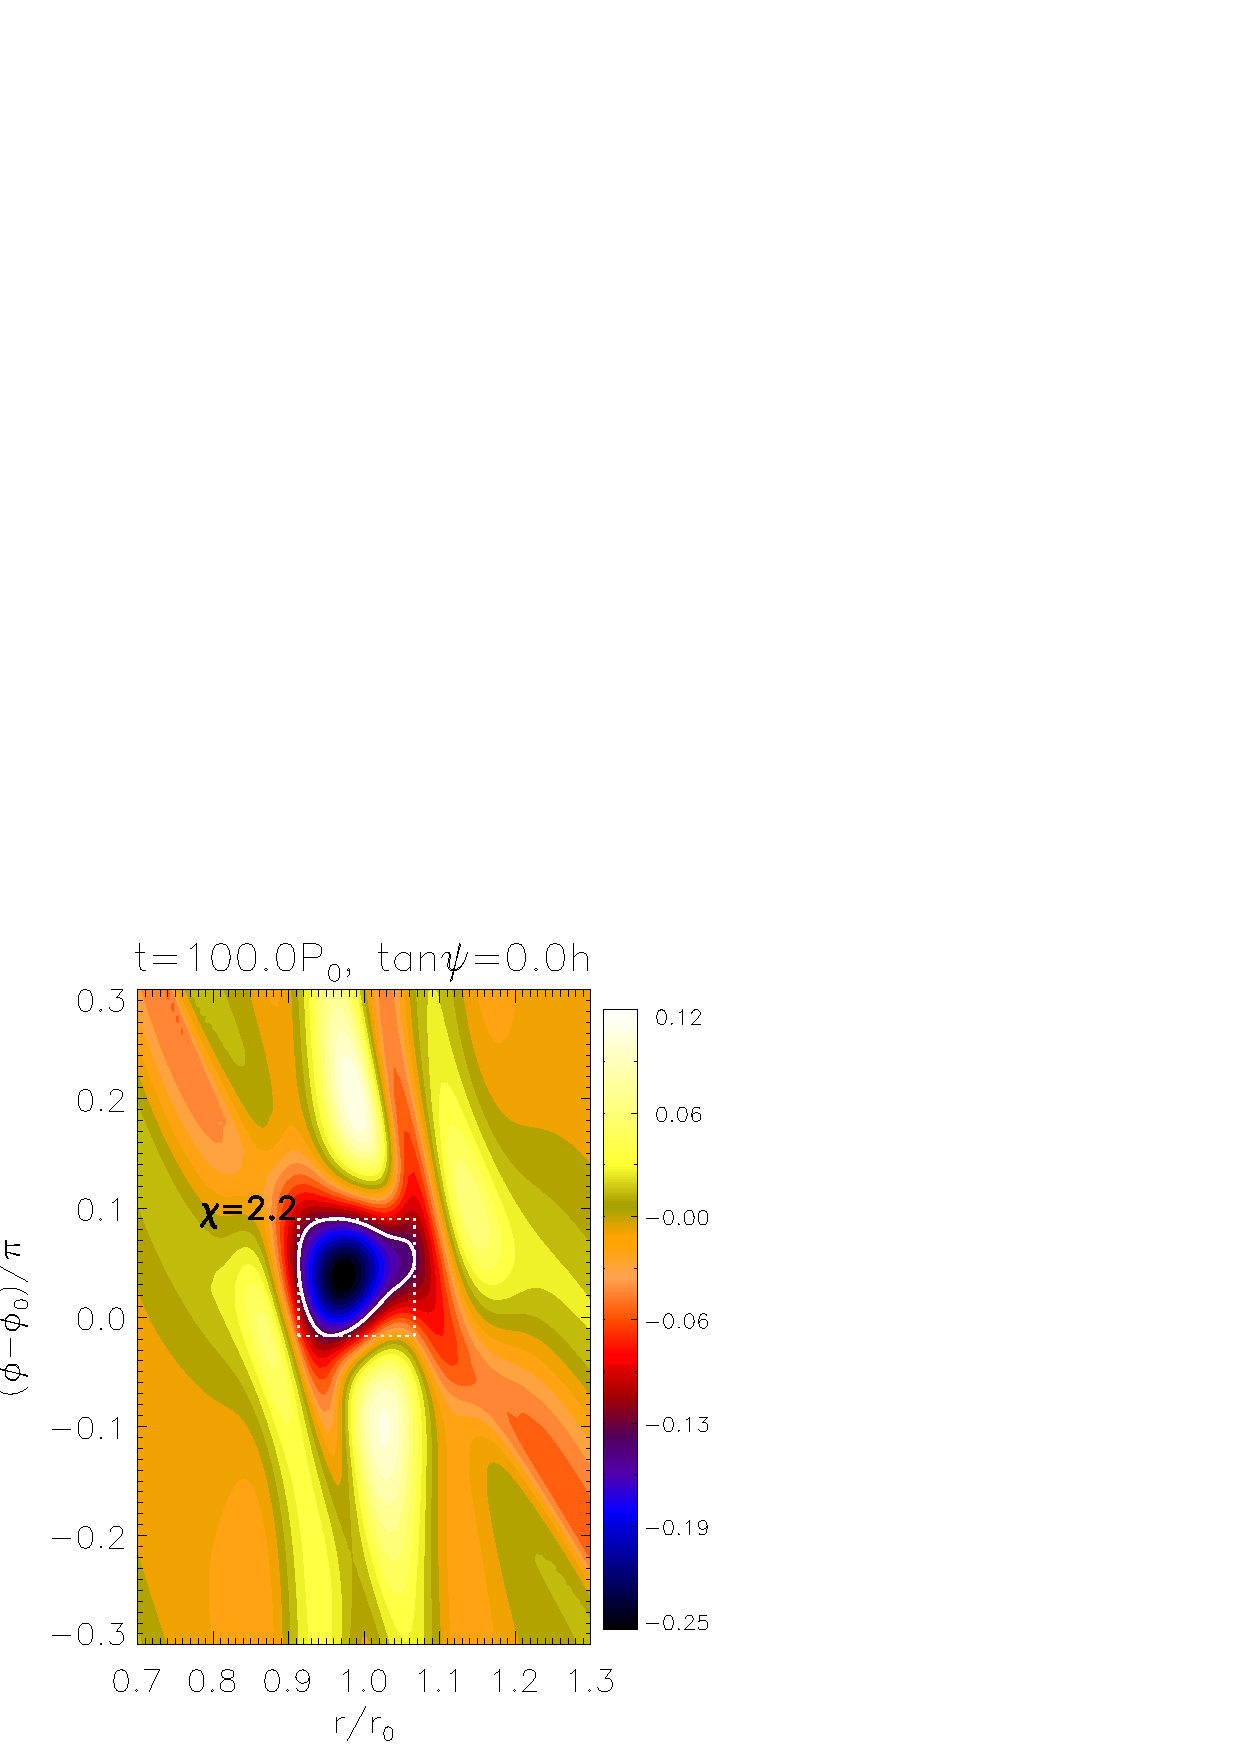
\includegraphics[scale=.27,clip=true,trim=2.3cm
   %%   0.cm 0.cm
   %%   0.99cm]{figures/vdamp0_nu4_vort019}\includegraphics[scale=.27,clip=true,clip=true,trim=2.3cm
   %%    0.cm 0.cm
   %%    0.99cm]{figures/vdamp0_nu4_vort024}
    \caption{Same as Fig. \ref{vdamp2} but for the midplane Rossby
      number $Ro(z=0)$. The vortex becomes smaller as the thickness of
      the upper viscous layer is increased (left to right).  
      \label{vdamp2_vort}}
\end{figure}

Stronger vortical structures with increasing viscosity is somewhat counter-intuitive, 
as one normally expects viscosity to smooth out the flow. To
rationalize this observation, we recall that the instability is
fundamentally associated with vortensity minima. Consider the
vortensity perturbation at the bump radius, which was found to be 
\begin{align}
  \left.\frac{\aziavg{\eta_z}(t=100P_0)}{\eta_z(t=0)}\right|_{R=r_0} - 1 = 
  \begin{cases}
   3.01  & \text{Case V1} \\
   2.85  & \text{Case V2} \\
   1.82  & \text{Case V3} \\
  \end{cases}.
\end{align} 
(This value is $3.96$ for case V0.) The initial vortensity minimum is
therefore weakened by the instability in the non-linear regime
\citep{meheut10}. However, with increasing viscosity, this effect
diminishes. Since viscosity reduces the linear growth rate (Table
\ref{artificial_bump}), the disturbance saturates at a lower amplitude
\citep{meheut13}. This is expected to affect the background
axisymmetric state to a lesser extent.  

We also recall that in the present simulations, 
the viscosity profile was chosen to be
approximately consistent with a steady-state disc containing a
localised vortensity minimum.  We suggest that for
such setups, viscosity attempts to restore the initial disc profile,
which in turns support vortex formation over the local viscous
time-scale.  


When viscosity is small, the viscous time-scale is long. In this case
the non-linear evolution of the instability weakens the vortensity
extrema with viscosity playing no role. 
As we increase viscosity, the local viscous time-scale
becomes shorter than our simulation time-scale. This means that over
the course of the simulation, our spatially-fixed viscosity profile acts
as a source of vortensity minimum. In essence, in the non-linear
regime there is competition
between destruction of the initial vortensity minimum by the 
instability, and reformation of the initial vortensity minimum by the
imposed viscosity profile. 

%% Although the linear instability growth rate is smaller with increasing
%% viscosity,
%So over the course of
%the simulation, viscosity resists the weakening of the initial
%vortensity extrema by the instability.    
